\chapter{Experimental Results}
In this final chapter, we will analyze the results of the
models previously described by comparing their respective
test phases, highlighting any issues and strengths of the model.
We will test their performance using the Test Set,
as described in Section~\ref{sec:datasetsplitting}, and
evaluate them using different metrics.
Among these metrics, we will employ MAE (Mean Absolute Error) and MAPE (Mean Absolute Percentage Error) \cite{metrics}
to highlight the difference between the model's predictions and
the ground truth and the $R^2$ (R-squared) \cite{metrics} index to understand how well
the model-predicted curve approximates the real one.
Here's a brief introduction to the indices we will use:

%In questo ultimo capitolo andremo ad analizzare i risultati dei modelli
%precedentemente descritti confrontando le rispettive fasi di training,
%mettendo in evidenza eventuali problemi e punti di forza del modello.
%Testeremo le perfoance di questi utilizzando il dataset di Testing, descritto
%nella Sezione~\ref{sec:datasetsplitting}, valutandoli impiegando alcune
%metriche come il MAE (Mean Absolute Error) per evidenziare la diferenza tra predizione del modello e la ground turth, e l'indice $R^2$ per capire
%quanto la curva predetta dal modello riesca bene ad approssimare quella reale.
%Di seguito una breve introduzione agli indici che utilizzeremo:

\begin{itemize}
	\item \textbf{Mean Absolute Error (MAE)}: This metric represents the average pointwise error that the model makes compared to the ground truth. It is expressed in kW.
	      %MAE dell'intero buco, indica in meda l'errore puntuale che il modello commette rispetto alla ground truth. Viene espresso in kW.
	\item \textbf{Mean Absolute Percentage Error (MAPE)} \cite{metrics}: It indicates the error of the model relative to the ground truth, measured in percentage. The calculation of this metric in our case can be quite problematic due to the presence of many values close to zero or exactly zero. Therefore, the calculation is performed by only considering non zero values. Specifically, in addition to the standard MAPE, we will employ a refined version named as MAPE@$k$. In this variant, the metric is calculated exclusively for values in the ground truth greater than $k$. This choice is driven by the distortion introduced in MAPE values when incorrect predictions are linked to the lowest values. Such predictions might exhibit low absolute errors, yet correspond to significantly high percentage errors.
	      %MAPE, indica in percentuale quanto è l'errore del modello rispetto la groundh truth, misurato in percentuale
	\item \textbf{$R^2$ (R-squared)}: This index quantifies how well the prediction curve approximates the ground truth. It helps us understand how well the model approximates the trend of the reference instant prediction. This varies between 0.0, the worst case, to an ideal value of 1.0 \cite{metrics}.
	      %({\bf (*VP* aggiungerei il range di variazione dell'indice, così è chiaro chi sono massimo e minimo raggiungibili.)}
	      %$R^2$, questo indice ci va a quantificare quanto bene la curva della predizione approssimi quella della ground truth. Ci permette di
	      %capire quanto bene il modello riesce ad approssimare l'andamento della predizione istantanea di riferimento.
	      %\item \textbf{Daily MAE} FORSE TOGLIERE: It is calculated only for individual days within the gap. This metric highlights the average daily error that the model makes, measured in kW.
	      %MAE giornaliero, viene calcolato solo sui singoli giorni del buco. Mette in evidenza l'errore giornaliero medio che commette il modello misurato in kW.
	      %\item \textbf{Global MAE}: This is the average of all daily errors, expressed in kW.
	      %Global MAE , è la media di tutti i gli errori giornalieri espresso in kW.

\end{itemize}

\section{Testing Procedure}
All models will be tested using the same test set  introduced in the previous Chapter~\ref{chap:datapreprocessing}. It's important to note that this dataset consists of 33 features, which have been carefully selected as described in Section~\ref{sec:featureselection}, and it contains all the data sampled at 15-minute intervals during the month of April (2880 records). Each model will be tested at least once on this set, according to its suitable input format and capabilities.

%Furthermore, the RNN and Transformer models will undergo additional testing with this set, but the gap size will be fixed at 2 days. This choice was made to facilitate comparisons with the MLP model, which has a rigid input structure. If necessary, the latter two models may also undergo further testing with variations or fixed gap sizes.
%{\bf (*VP* questo paragagrafo è scritto male... e mi pare abbastanza inutile visti i seguenti. )}

The testing procedure applied to the MLP and RNN models for the purpose of comparison (with a fixed 2-day gap size) will be conducted as follows: a 4-day time window will be applied to the testing dataset, shifting forward by 1 day at each iteration. This approach will generate a 2-day gap to predict, along with the corresponding day before and after. For example, consider the time interval from April 2nd to April 5th (time window). In this case, the gap to predict includes all the data of April 3rd and April 4th, while April 2nd and April 5th are used, respectively as the data before and after the gap.

For the Transformer model, the testing procedure will be similar, with the only difference being the size of the time window. In the case of the Transformer, a 1-week time window will be used, and it will shift forward by 1 day at each iteration due to the model's input format requirements. This approach will ensure that a 2-day gap with relevant data before and after is available for the Transformer model as well.

%Tutti i modelli verranno testati con lo stesso testing set (Aprile 2023) introdotto nel precedente Capitolo~\ref{chap:datapreprocessing}. Ricordiamo come questo è composto da 33 features, che sono state accuratamente selezionate come descritto in sezione~\ref{sec:featureselection}, e contine dati campionati ad un itervallo di 15 minuti. Ogni modello verrà testato almeno una volta su questo set nelle modalità più consone e secondo l'input richiesto ed in base alle sue capacità. Poi i modelli RNN e Transformer verranno ulteriormente testati, sempre con questo set, andando però a fissare la lunghezza dei buchi creati a 2 giorni in moto tale da poter essere confrontati successivamente con MLP data la sua rigidità nell'input. Qual'ora fosse necessario, questi ultimi due, potrebbero essere testati ulteriormente andando a variare o fissare la gap size.
%
%La procedura di testing che verrà applicata ai modelli MLP e RNN per essere poi confrontati (gap size fissa a 2 giorni) si svolgerà nel seguente modo: avremo una finestra temporale di 4 giorni che verrà applicata al dataset di testing e scorrerà sempre di 1 giorno in avanti. In questo modo potremmo ottenere, per tutti i modelli, un buco di 2 giorni e il relativo giorno prima e dopo. Per esempio, prendiamo l'intervallo di tempo che va dal 2 Aprile fino al 5 Aprile (finestra temporale). In questo caso il buco da predirre sarà relativo ai giorni 3 e 4, mentre avremo il 2 e il 5 come prima e dopo.
%Mentre per il transformer cambierà solo la dimensione della finestra temporale, che sarà di una settimana e si sposterà in avanti di 1 giorno, per via del formato dell'input che richiede il modello.
%\newpage


\section{MLP}\label{sec:mlpbaseline}
In this section, we will introduce the first model, which we will refer to as the
baseline model, based on a Multi-Layer Perceptron.
We will analyze its architecture, the training phase, and its final performance.

%In questa sezione andremo ad introdurre il primo modello a cui faremo
%riferiento come baseline model, basato su MultiLayer Perceptron.
%Analizzeremo la sua architettura, la 
%fase di training e le sue performance finali.

\subsection{Architecture}
This neural network is designed to predict the instantaneous energy output over
a period of exactly 2 days.
To do this, it requires input data that includes the performance of the system
(features selected during the Preprocessing phase, see Chapter \ref{chap:datapreprocessing}) for exactly one day
before and one day after the period in question.
This enables it to understand how the system is performing and,
consequently, provide the energy output trend.
The model consists of 6 main layers:

%Questa rete neurale è progettata per prevedere l'andamento dell'energia istantanea prodotta durante un periodo di un buco di esattamente 2 giorni.
%Per farlo ha bisogno di avere come input l'andamento dell'impianto (features selezionate nella fase di preprocessing) di esattamente un giorno prima del
%buco e di un giorno dopo. In questo modo può riuscire a comprendere come l'impianto sta performando e quindi restituire l'andamento dell'energia.
%Il modello è formato da 6 livelli principali:

\begin{figure}[H]
	\begin{minipage}{0.6\textwidth}
		\begin{itemize}
			\item \textbf{Input layer}: This is the first layer of the network.
			      It takes two input tensors: \textit{before} and \textit{after}.
			      These tensors represent the day before and the day after the specific period we want to
			      predict. They have the shape \verb|[BATCH_SIZE, 96, 33]|, where 96 is the number
			      of timestamps in our dataset that make up one day, and 33 represents the
			      features obtained from the Data Preprocessing phase.
			      These tensors are then flattened and concatenated to be passed to the subsequent layer.
			      The output of this layer goes through a Batch Normalization layer, and the
			      Rectified Linear Unit (ReLU) activation function is used.

			      % è il primo livello della rete, prende in input 2 tensori: \textit{before} e \textit{after}. Questi stanno ad indicare rispettivamente il giorno prima e quello dopo del buco che vogliamo chiudere. Avranno la forma \verb|[BATCH_SIZE, 96, 33]|, dove \verb|96| è il numero di timestamp del nostro dataset che formano un giorno e \verb|33| sono le feature ottenute dalla fase di preprocessing dei dati. A questi verrà poi applicata un'operazione di Flatten ed infine concatenati per poter essere poi passati al layer successio.
			      %L'output di questo layer passa per un livello di Batch Normalization e viene utilizzata la ReLu come funzione di attivazione. 

			\item \textbf{Hidden layers}: In total, there are 4 layers, each of which takes the
			      output of the previous layer as input and reduces the number of neurons by half.
			      Batch Normalization is applied to the result, and the Rectified Linear Unit (ReLU)
			      is used as the activation function.

			      %in totale 4, ognuno prende in input il risultato del layer precedente e va a dimezzare il numero dei neuroni. Al risultato viene applicata un'operazione di Batch Normalization e utilizzata la ReLu come funzione di attivazione.

			\item \textbf{Output layer}: The final layer of our network, it takes the result from the
			      previous layer and outputs the value of the Instantaneous Energy Produced
			      during the specific period.
			      It produces a tensor with a shape of \verb|[BATCH_SIZE, 192, 1]|.
			      The SoftPlus function is used as the final activation function.

			      %ultimo layer della nostra rete, dal risultato del layer precedente riporta come output il valore dell'Energia Istantanea Prodotta durante il buco, un tensore di forma \verb|[BATCH_SIZE, 192, 1]|. Viene utilizzata la SoftPlus come funzione di attivazione finale.
		\end{itemize}
	\end{minipage}%
	\hspace{0.5cm}
	\begin{minipage}{0.4\textwidth}
		\centering
		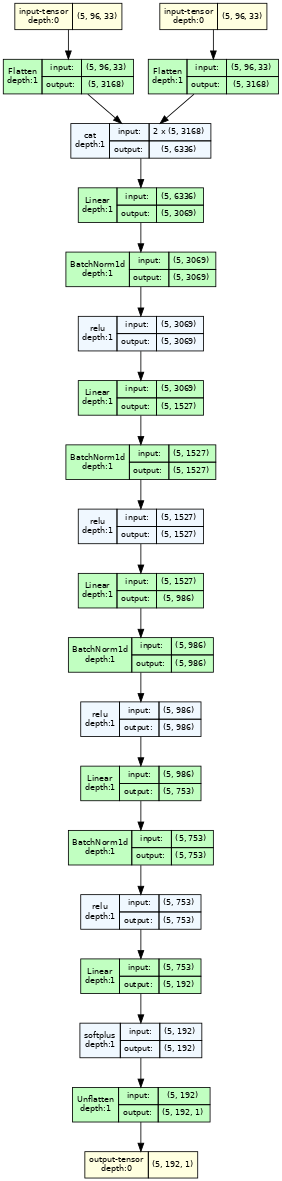
\includegraphics[width=0.5\textwidth]{chapters/3_models/imgs/ufcnmodel.png}
		\caption{Beseline Model architecture visualization.}\label{fig:baselinemodelarch}
	\end{minipage}
\end{figure}

\begin{minipage}[t]{0.5\textwidth}
	\begin{figure}[H]
		\centering
		\begin{tikzpicture}
			\draw[->] (-3,0) -- (3,0) node[right] {$x$};
			\draw[->] (0,-1) -- (0,4) node[above] {$y$};
			\draw[dotted] (-3,-1) grid (3,4);
			\draw[color=blue, domain=-3:0] plot[id=logistic] function{0};
			\draw[color=blue, domain=0:3] plot[id=logistic] function{x};
		\end{tikzpicture}
		\caption{Rectified Linear Unit function. $ReLu(x) = \max(0, x)$}
		\label{fig:relu}
	\end{figure}
\end{minipage}%
\hspace{.5cm}
\begin{minipage}[t]{0.5\textwidth}
	\begin{figure}[H]
		\centering
		\begin{tikzpicture}
			\draw[->] (-3,0) -- (3,0) node[right] {$x$};
			\draw[->] (0,-1) -- (0,4) node[above] {$y$};
			\draw[dotted] (-3,-1) grid (3,4);
			\draw[color=blue, domain=-3:3] plot[id=logistic] function{log(1+exp(x))};
		\end{tikzpicture}
		\caption{SoftPlus function. $SoftPlus(x) = \frac{1}{\beta} \log(1+e^{\beta x})$}
		\label{fig:softplus}
	\end{figure}
\end{minipage}

\subsection{Training}
The model was trained by artificially creating gaps of two days in length within the
training dataset.
These gaps were passed to the network in the format described earlier,
and the output result was compared to the actual instantaneous energy produced during the gap.
An \textit{Early Stopping} procedure was implemented to prevent training from continuing if
the model was not improving its performance.
A procedure, called \textit{Save Best}, has also been integrated,
which saves the model to a file whenever the Validation Loss improves.
The validation dataset was applied in this phase to assess the learning progress at the end
of each epoch.
A normalization procedure of the area was applied to the model's output in relation to
that of the gap to ensure that the output starts exactly from the last value of the
instantaneous energy produced \textit{before} and ends exactly with the first value
of the energy produced \textit{after}. Adam was used as the optimizer,
and L1Loss (Equation~\ref{eq:l1loss}) served as the loss function.
We chose to set the batch size parameter to 10, the learning rate $\lambda$ to 0.01,
a maximum of 100 epochs, and a patience value of 20 for Early Stopping.

%Il modello è stato allenato creando, in modo artificiale, buchi di lunghezza
%pari a due giorni all'interno del dataset di training, passati alla rete nel formato
%descritto precedentemente e confrontato il risultato in output con l'effettiva energia istantanea
%prodotta del buco. \'{E} stata implementata una procedura di \textit{Early Stopping} per evitare
%di continuare l'allenamento anche se il modello non sta migliorando le sue performance. 
%\'{E} stata anche integrata una procedura, chiamata \textit{Save Best},
%che salva il modello su file ogni qualvolta la validation loss migliori.
%Il dataset di validation è stato applicato in questa fase per verificare lo stato di
%apprendimento alla fine di ogni epoca. All'output del modello è stata applicata una 
%procedura di normalizzazione dell'area rispetto a quella del buco per far si che la predizione
%parta esattamente dall'ultimo valore dell' energia istantanea prodotta di \textit{before} e
%termini esattamente con il primo valore di \textit{after}.
%\'{E} stato impiegato Adam come ottimizzatore e la L1Loss (Equation \ref{eq:l1loss}) come loss function.
%Abbiamo scelto di impostare il parametro batch size a 10, learning rate $\lambda$ a 0.01, 100
%come numero massimo di epoche e 20 come patience per l'Early Stopping.

\begin{gather}\label{eq:l1loss}
	L = \{l_1,\dots,l_N\}^\top, \quad
	l_n = \left| x_n - y_n \right|,\\
	\ell(x,y) = \operatorname{mean}(L)
\end{gather}

\begin{table}[H]
	\begin{center}
		\begin{tabular}[c]{l|l}

			\textbf{Total Parameters (\#)}     & 26543400 \\
			\textbf{Trainable Parameters (\#)} & 26543400 \\
			\textbf{Training Duration (s)}     & 24.0     \\
			\textbf{Model Size (MB)}           & 101.3
		\end{tabular}
	\end{center}
	\caption{Baseline Model specification.}\label{tab:ufcnspecs}
\end{table}

\begin{figure}[H]
	\centering
	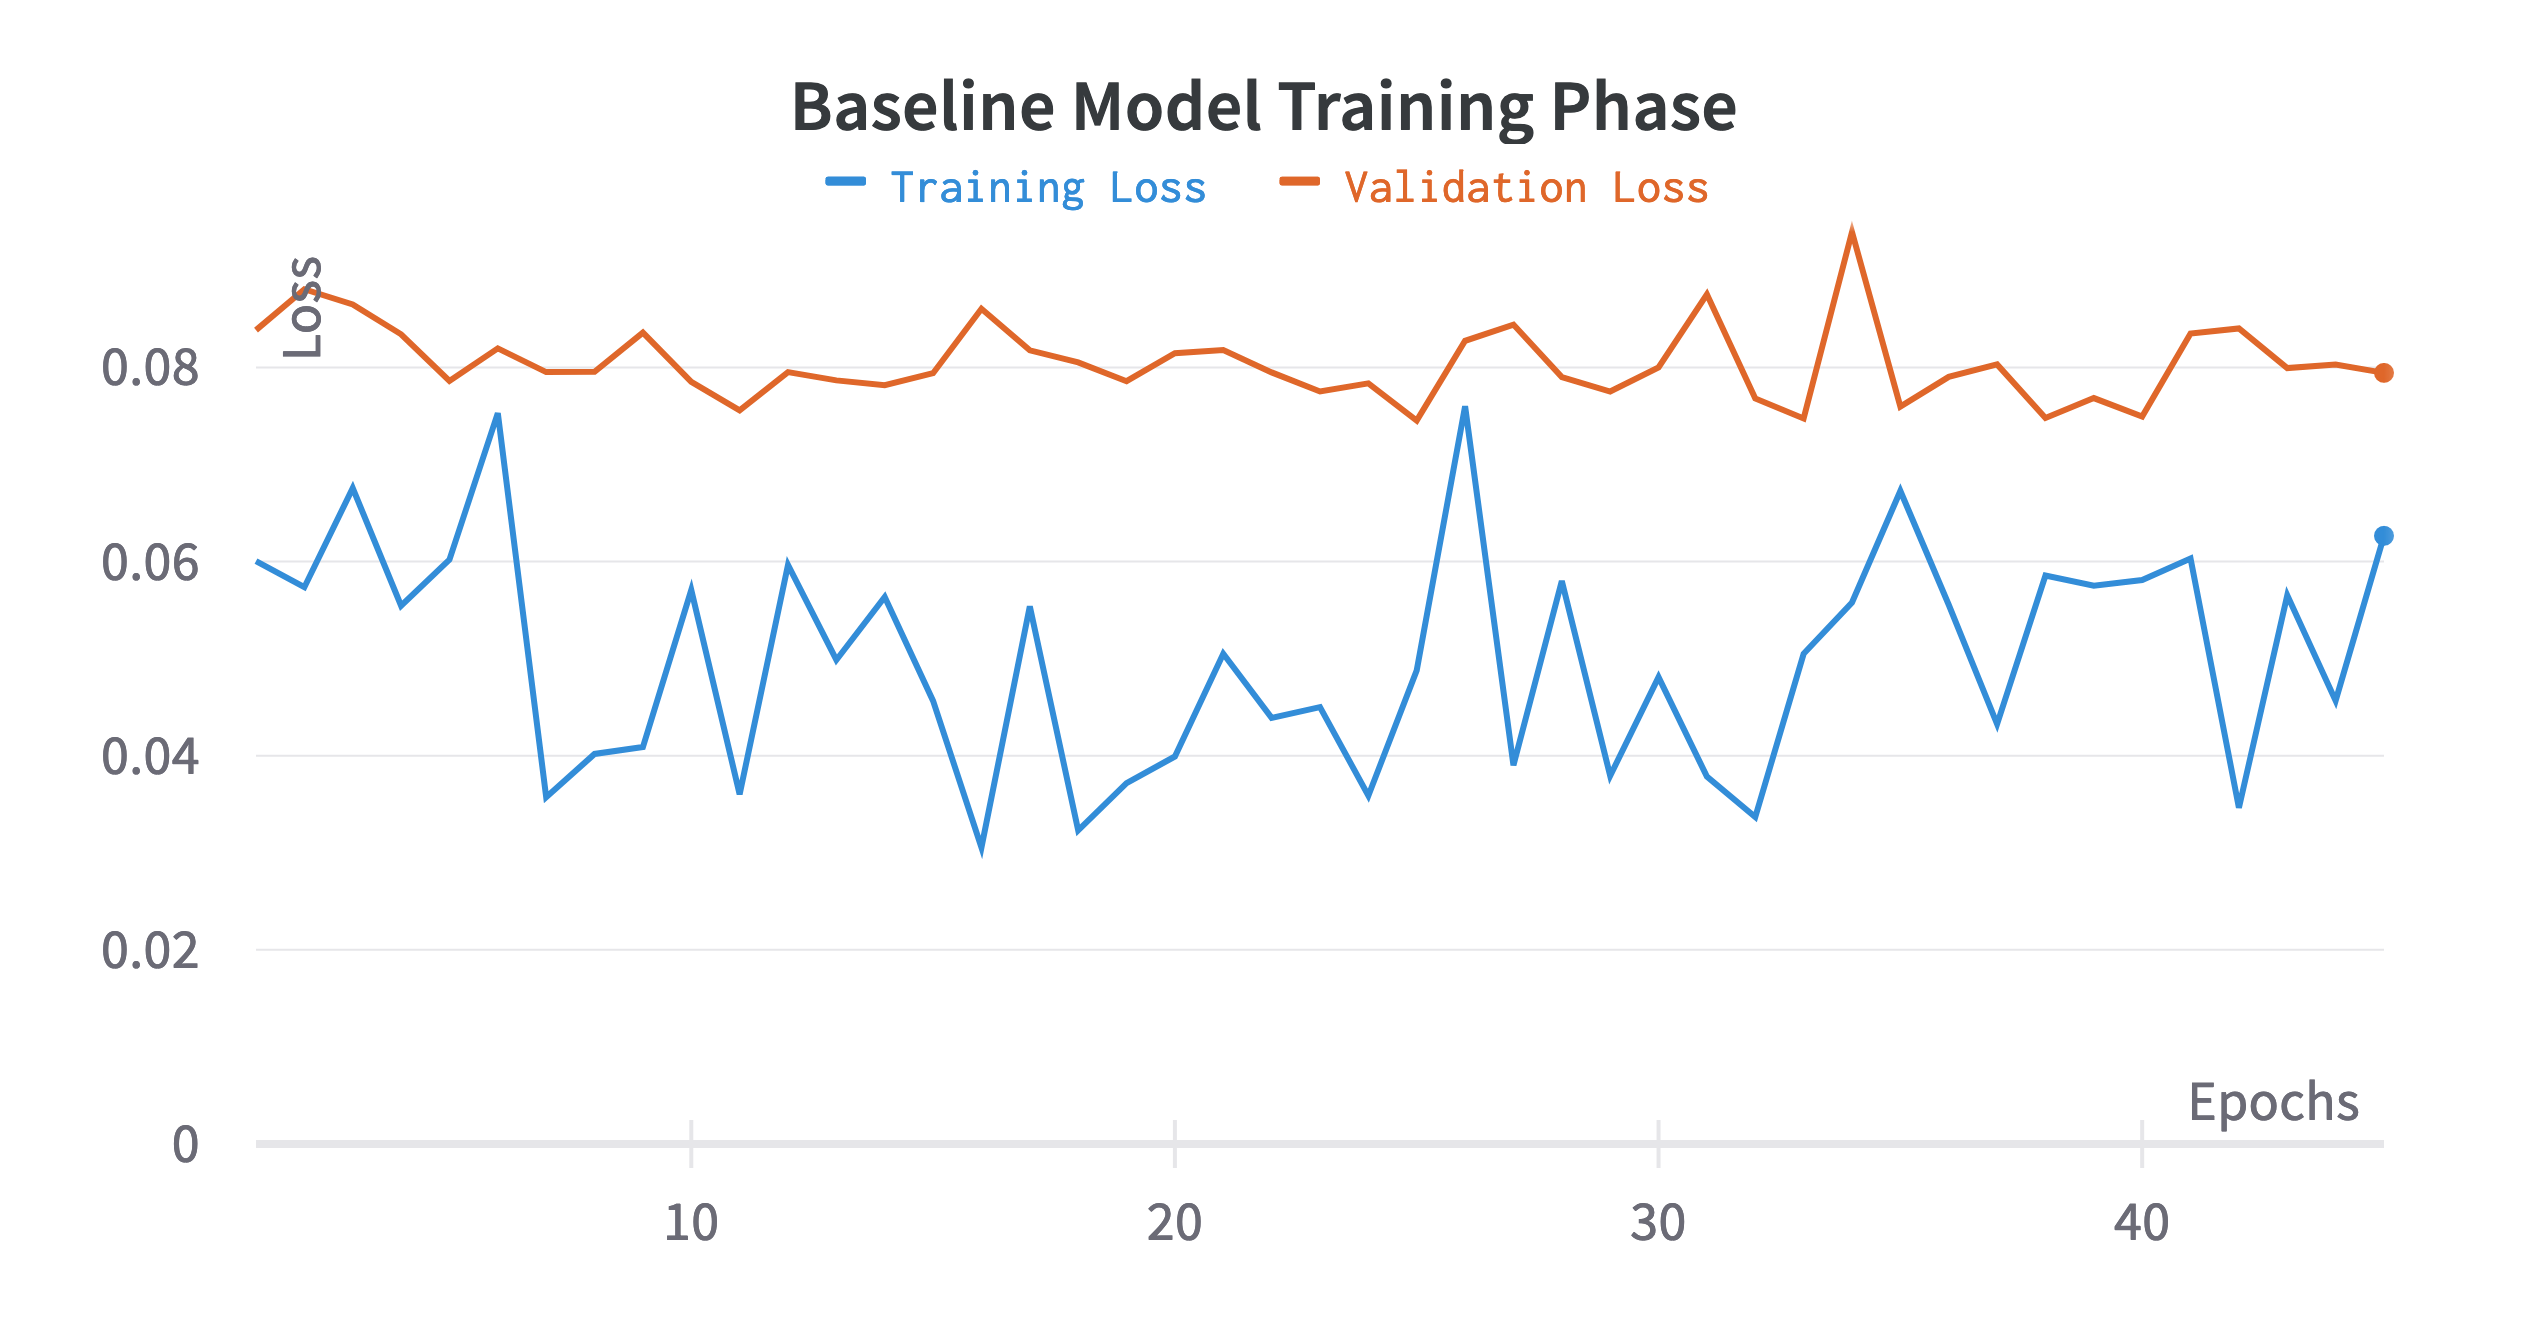
\includegraphics[width=\textwidth]{chapters/3_models/imgs/ufnc/ufnctraining.png}
	\caption{The chart displays the loss progression during the training phase. The blue line represents the Training Loss, while the orange line represents the Validation Loss.}
	\label{fig:ufcntraining}
\end{figure}

\begin{figure}[H]
	\centering
	\begin{subfigure}{0.32\textwidth}
		\centering
		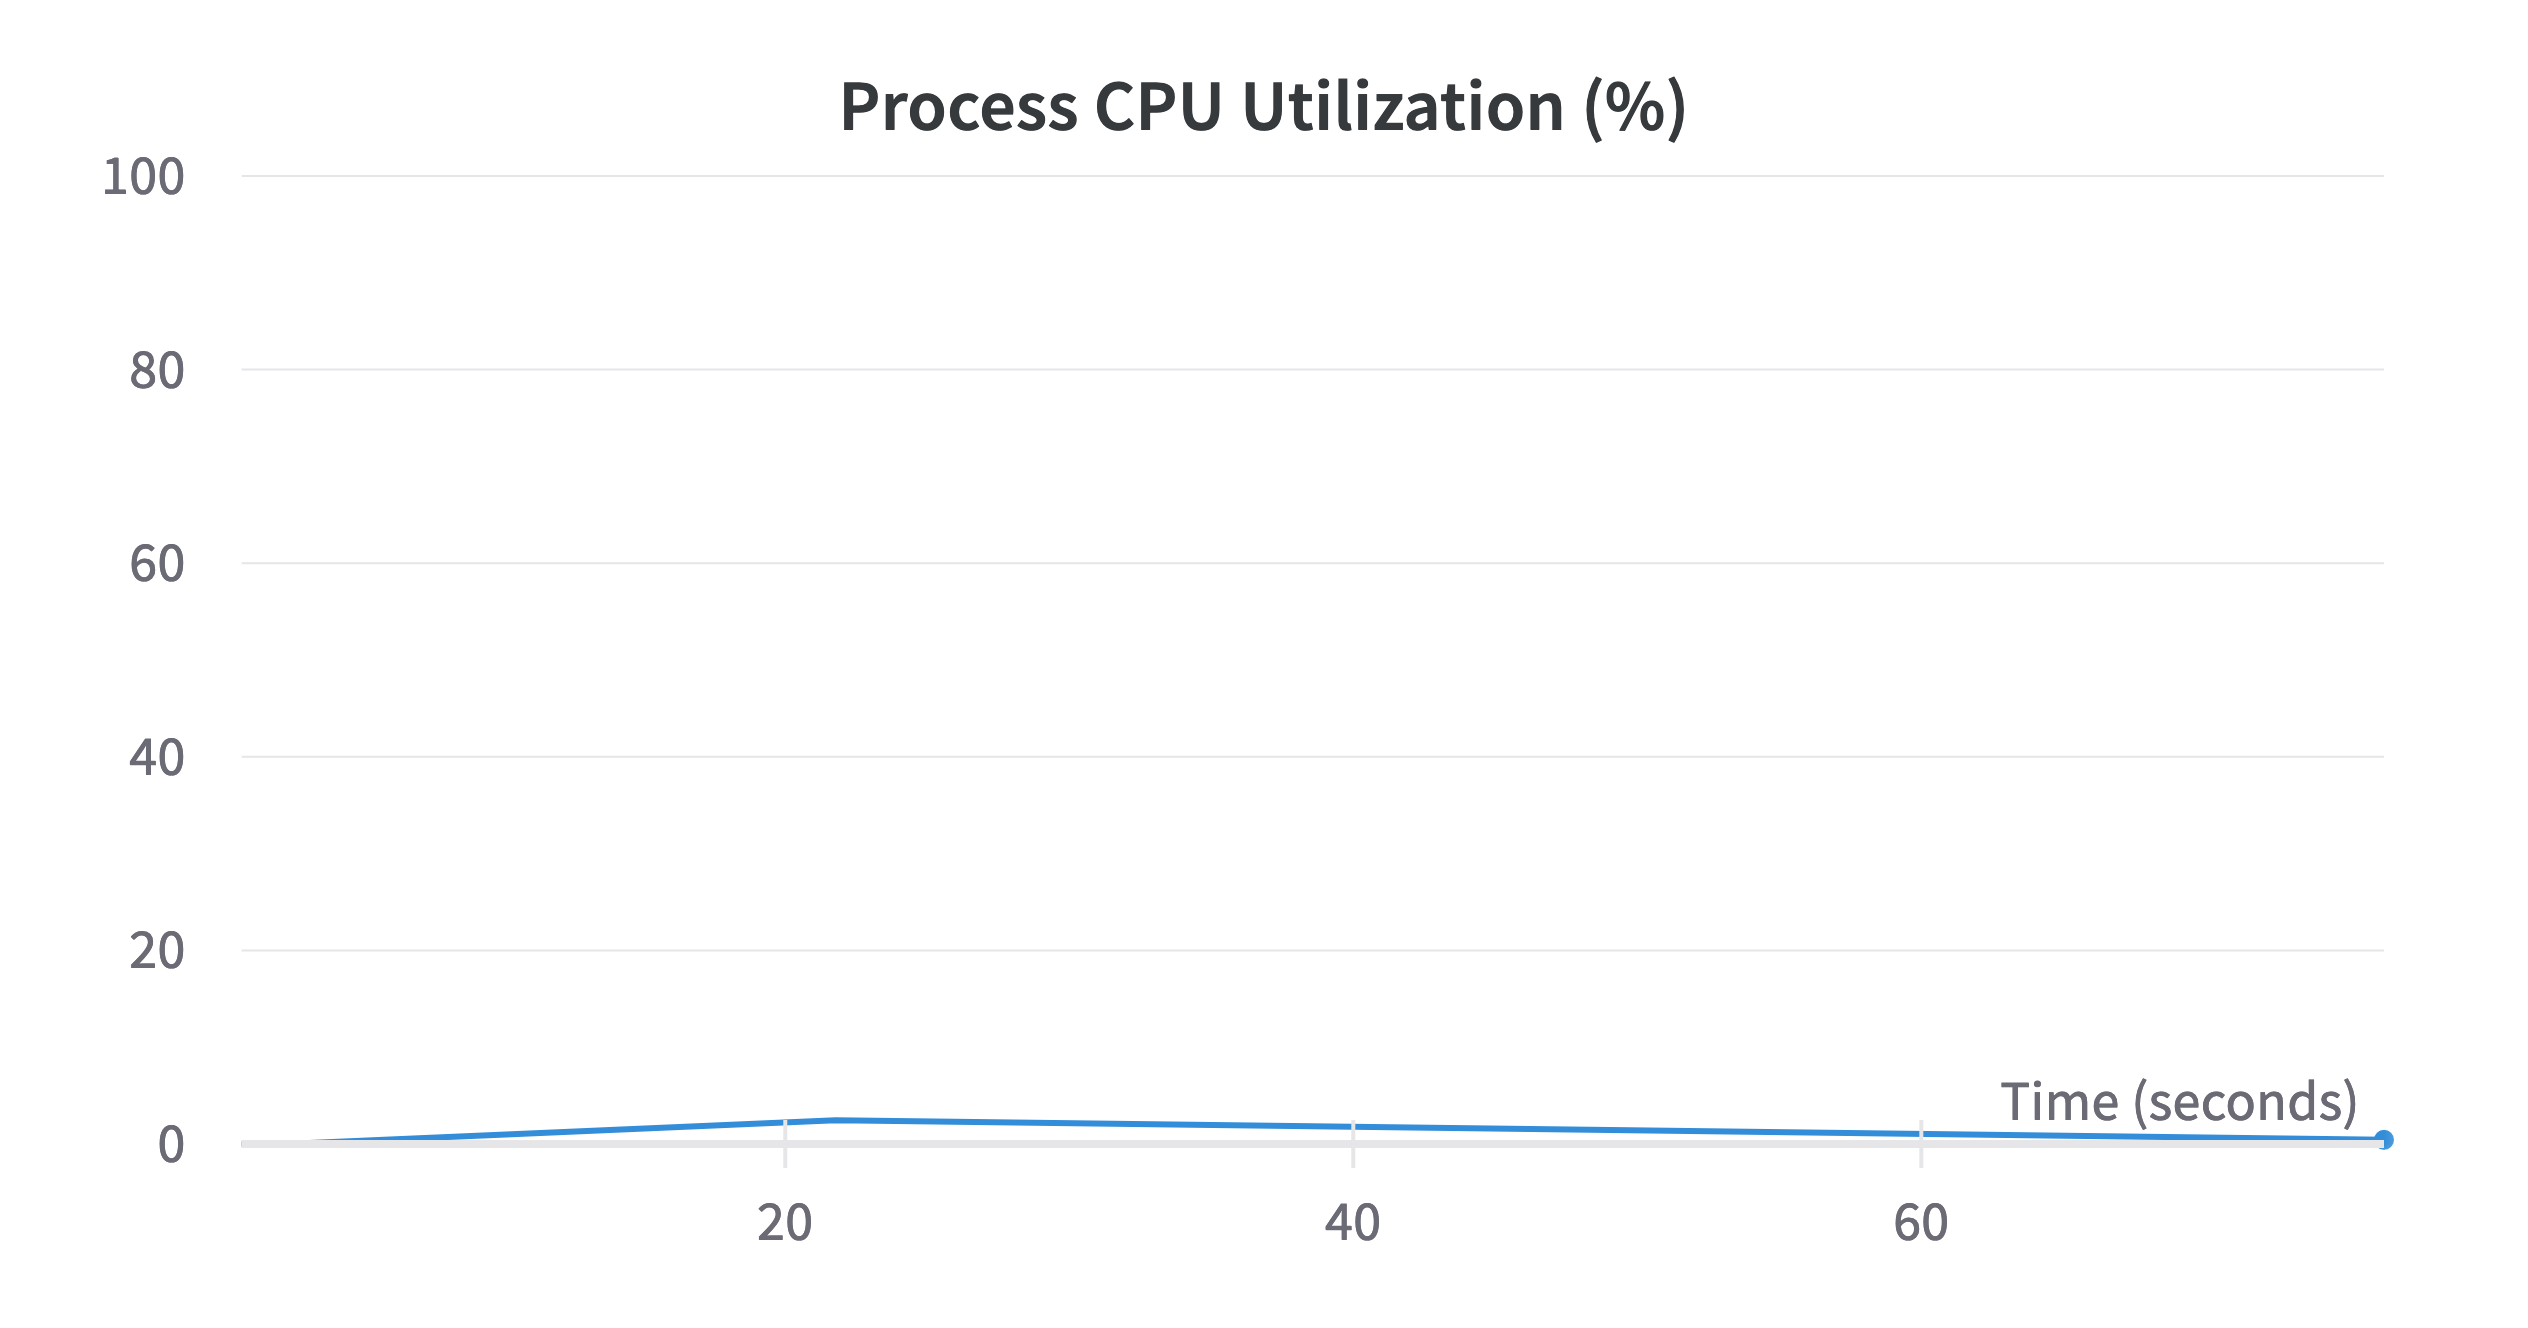
\includegraphics[width=\textwidth]{chapters/3_models/imgs/ufnc/ufcncpusage.png}
	\end{subfigure}
	\begin{subfigure}{0.32\textwidth}
		\centering
		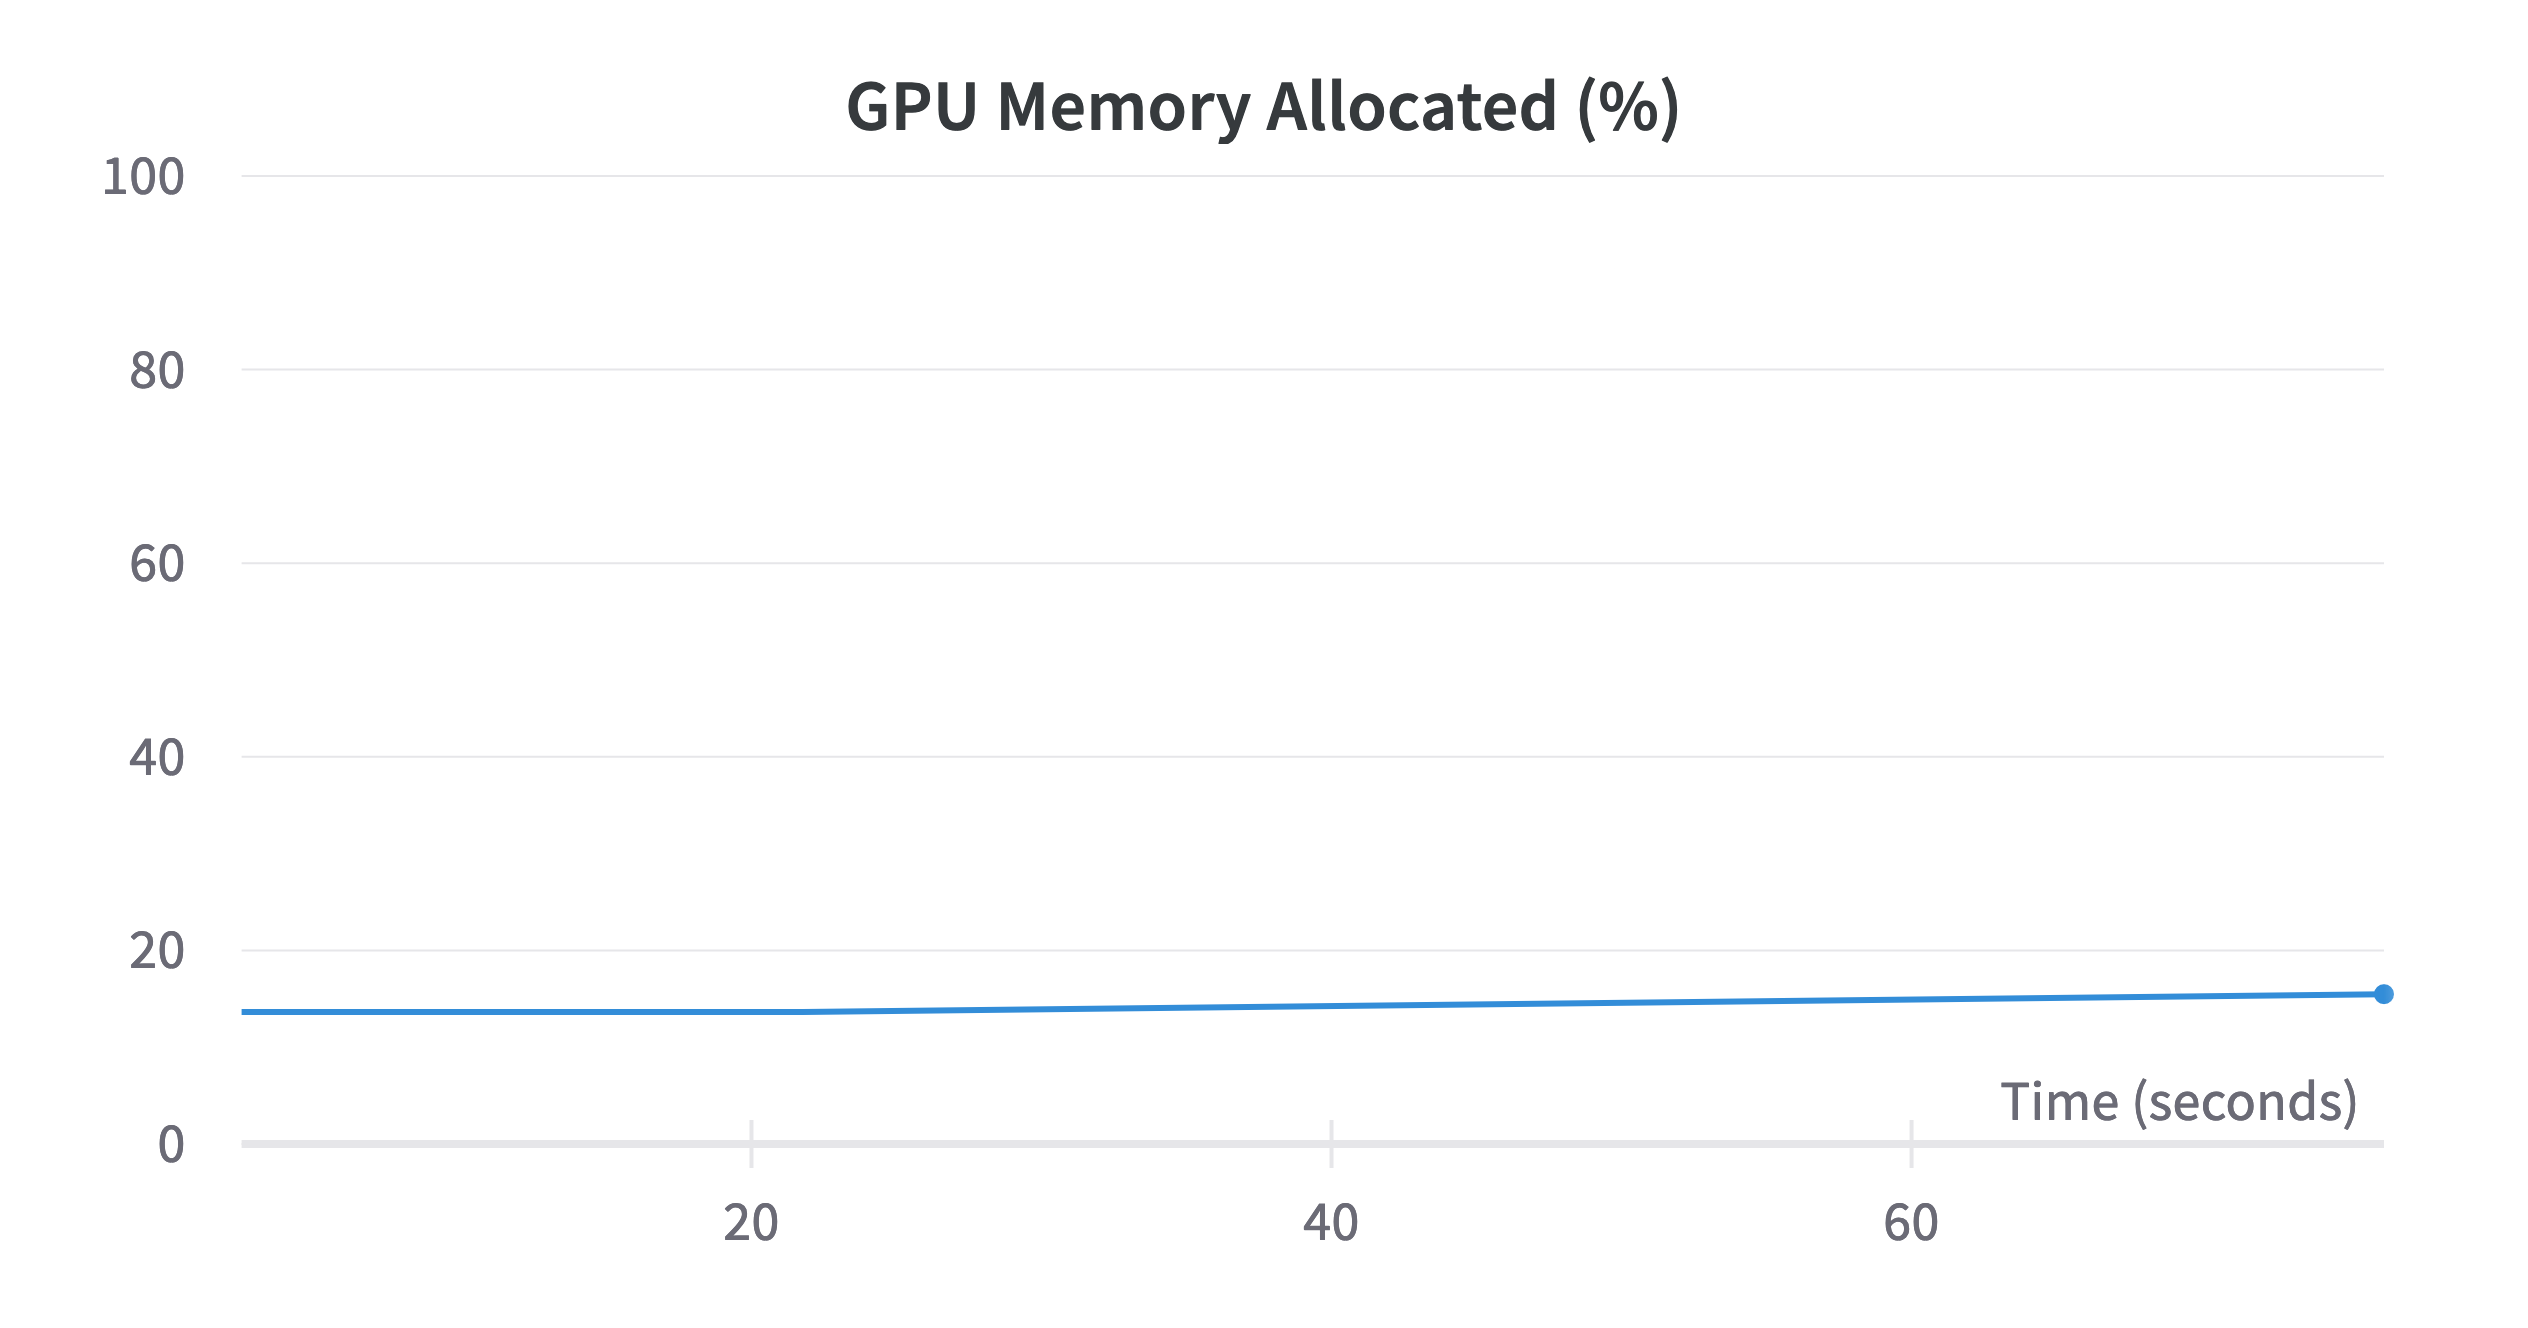
\includegraphics[width=\textwidth]{chapters/3_models/imgs/ufnc/ufcnmem.png}
	\end{subfigure}
	\begin{subfigure}{0.32\textwidth}
		\centering
		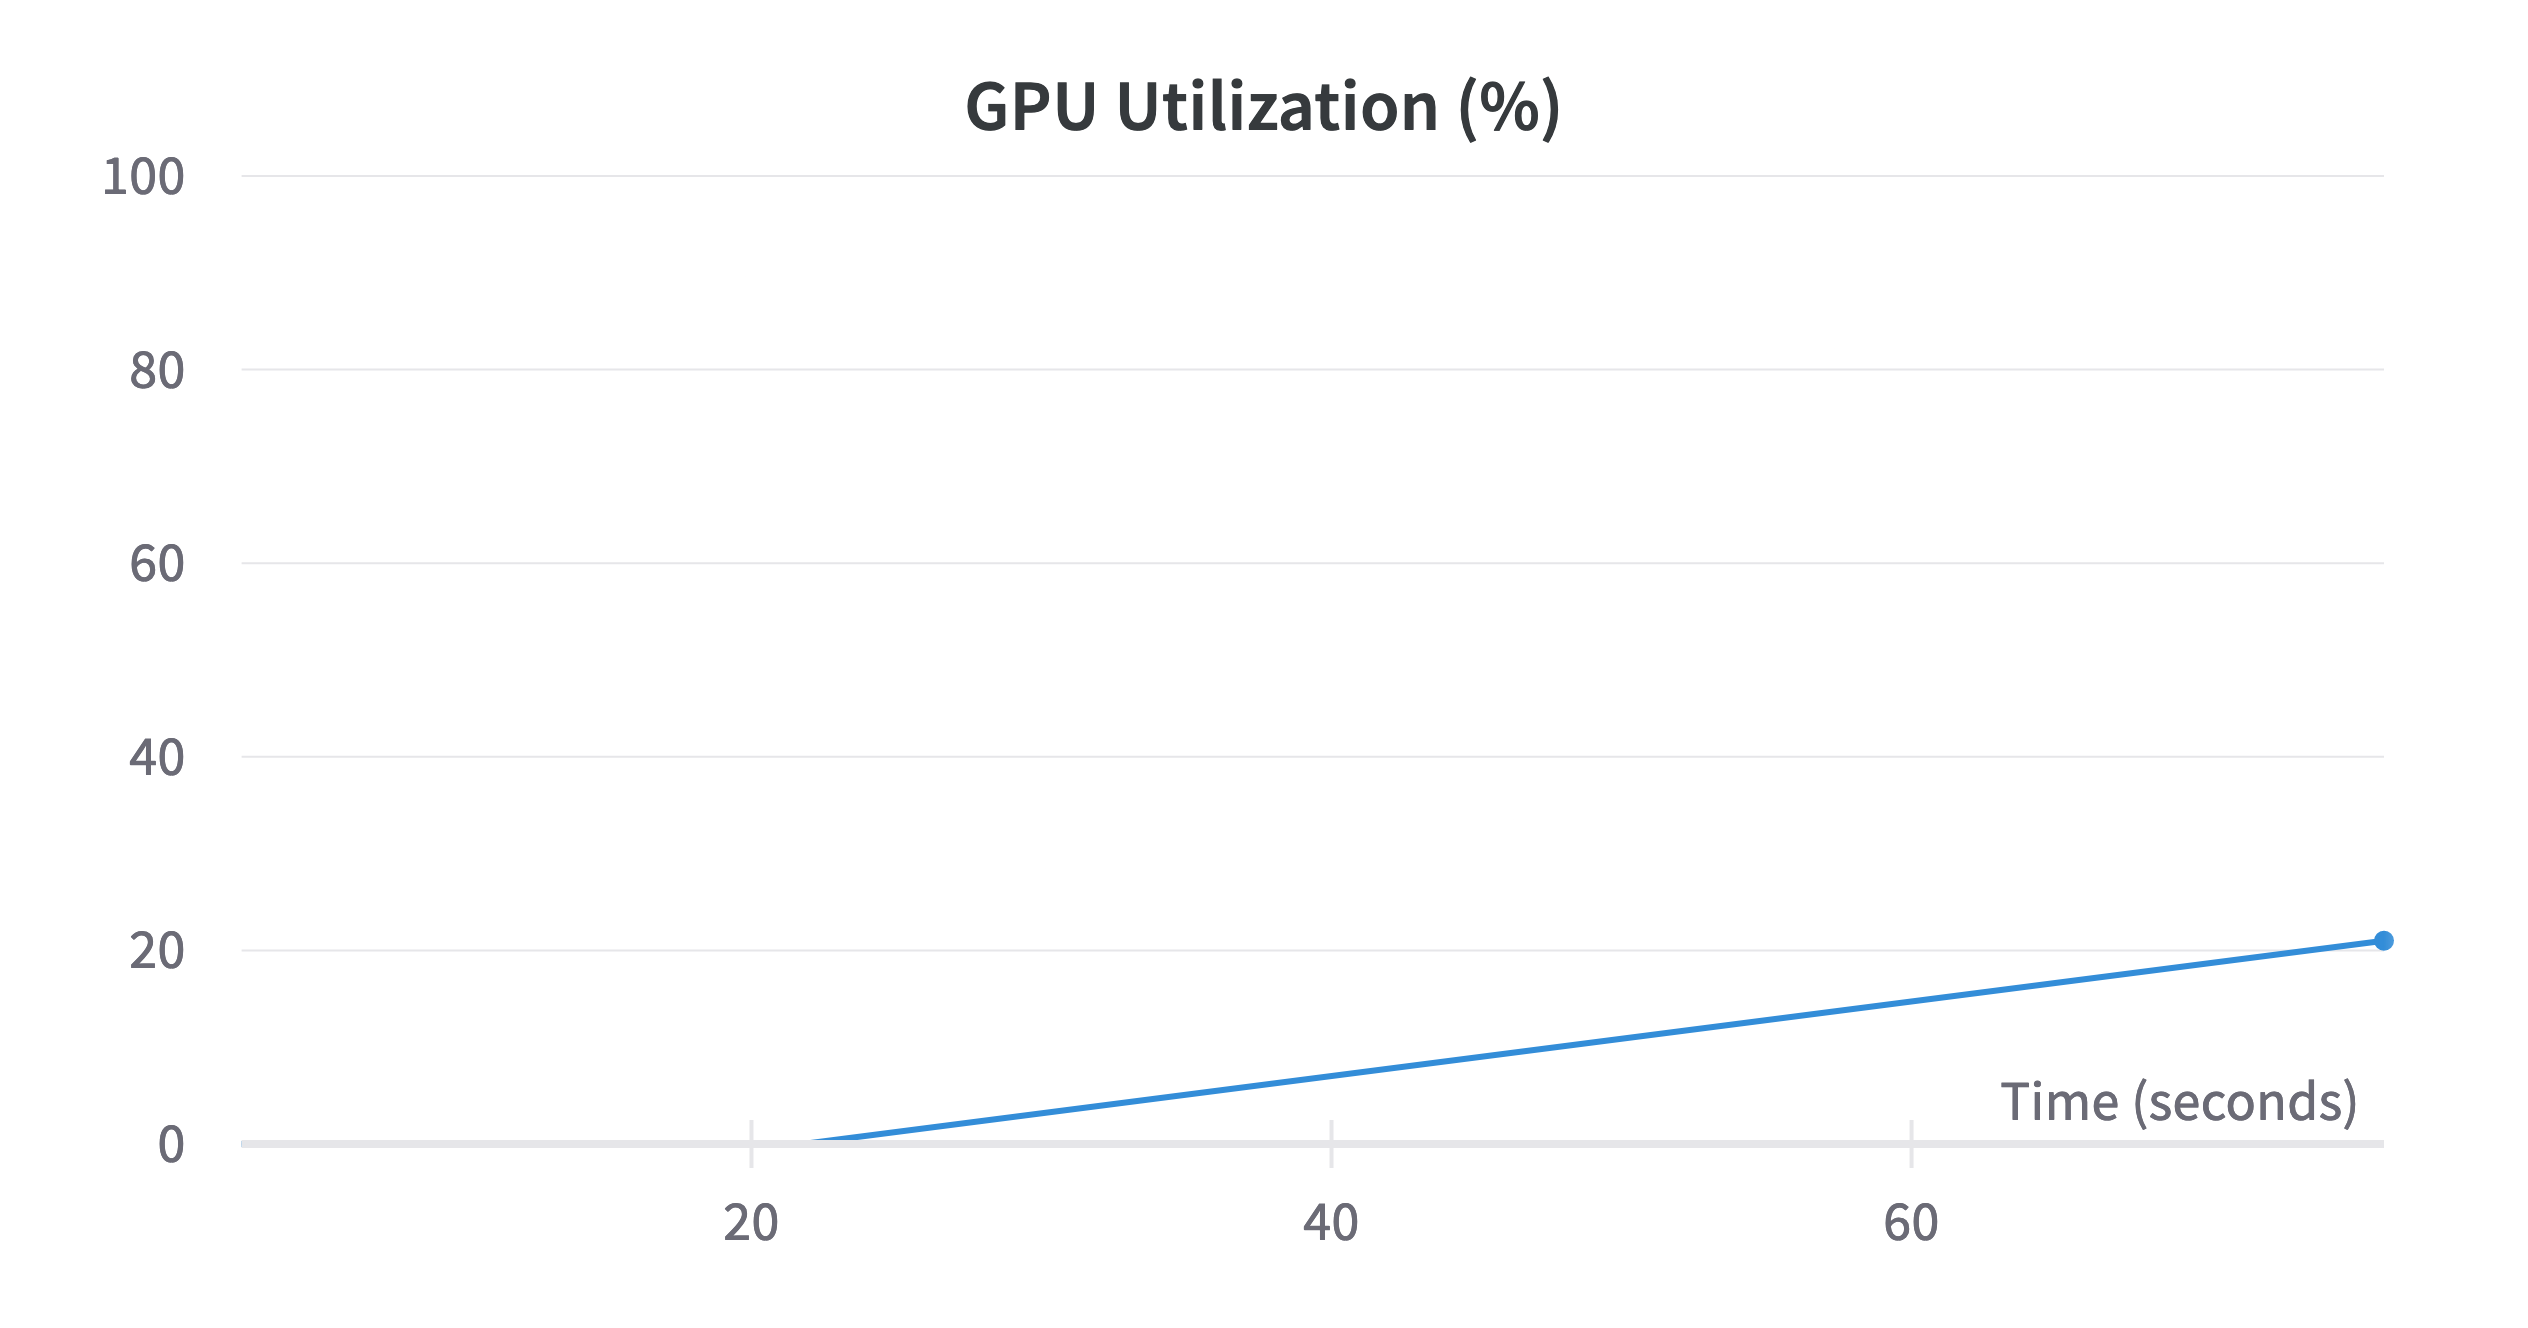
\includegraphics[width=\textwidth]{chapters/3_models/imgs/ufnc/ufcnusagevera.png}
	\end{subfigure}\\
	\begin{subfigure}{0.32\textwidth}
		\centering
		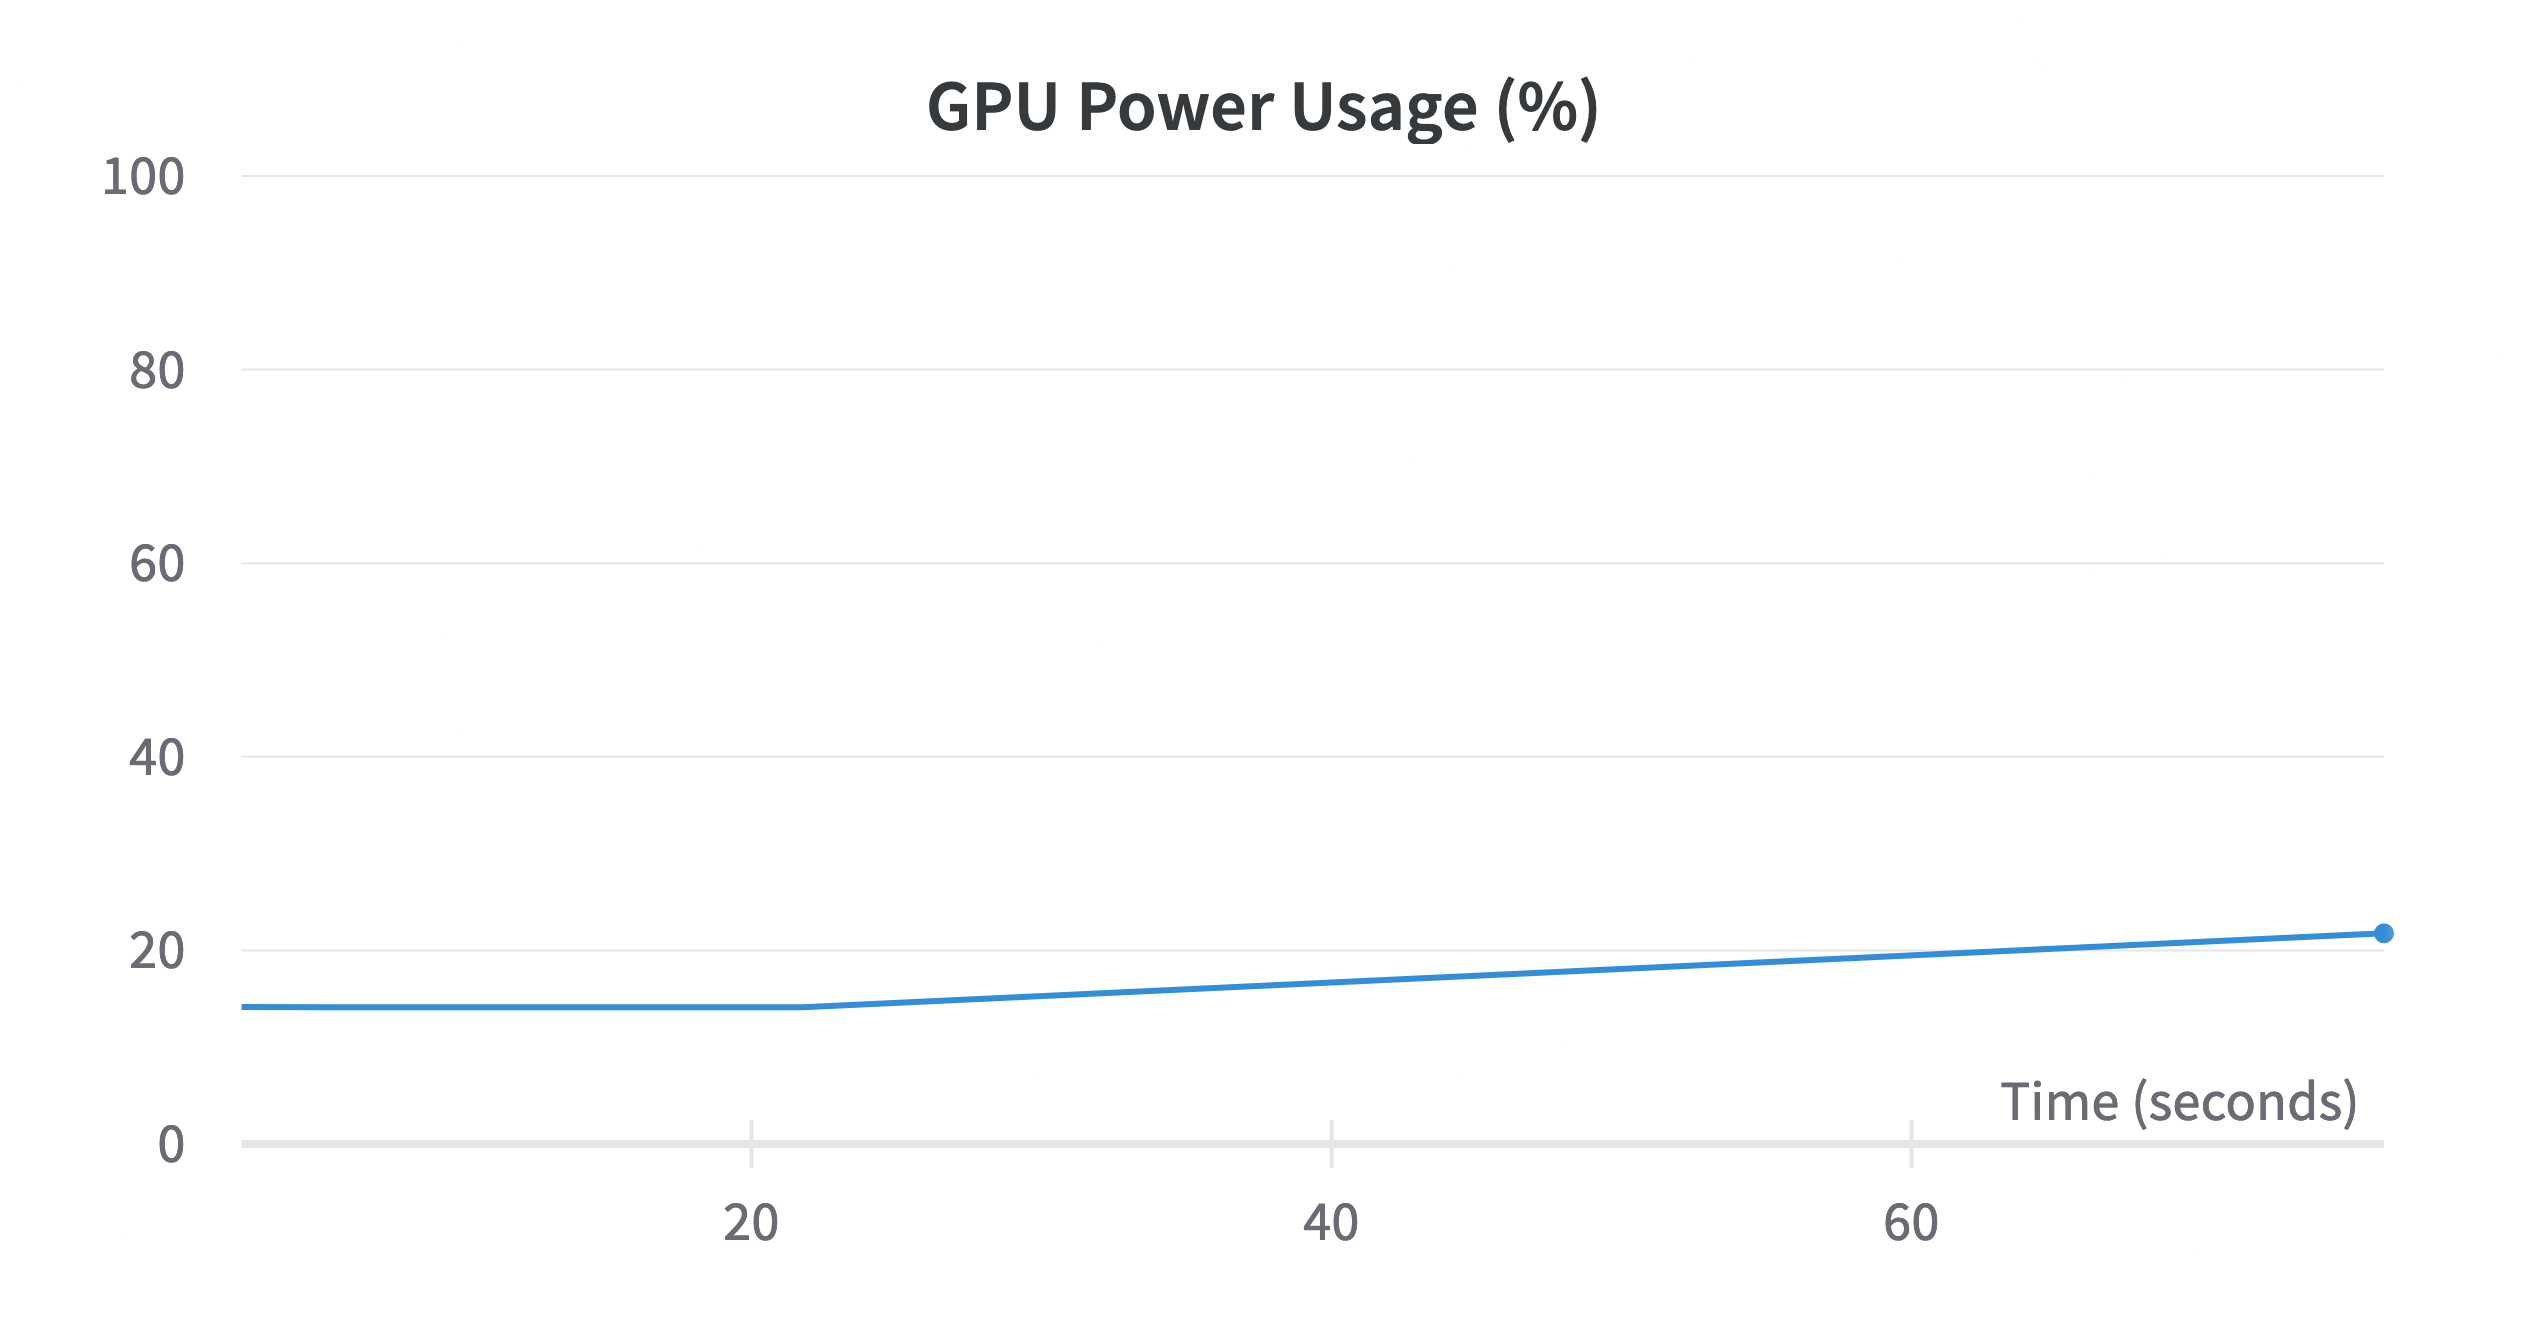
\includegraphics[width=\textwidth]{chapters/3_models/imgs/ufnc/ufncusageperc.png}
	\end{subfigure}
	\begin{subfigure}{0.32\textwidth}
		\centering
		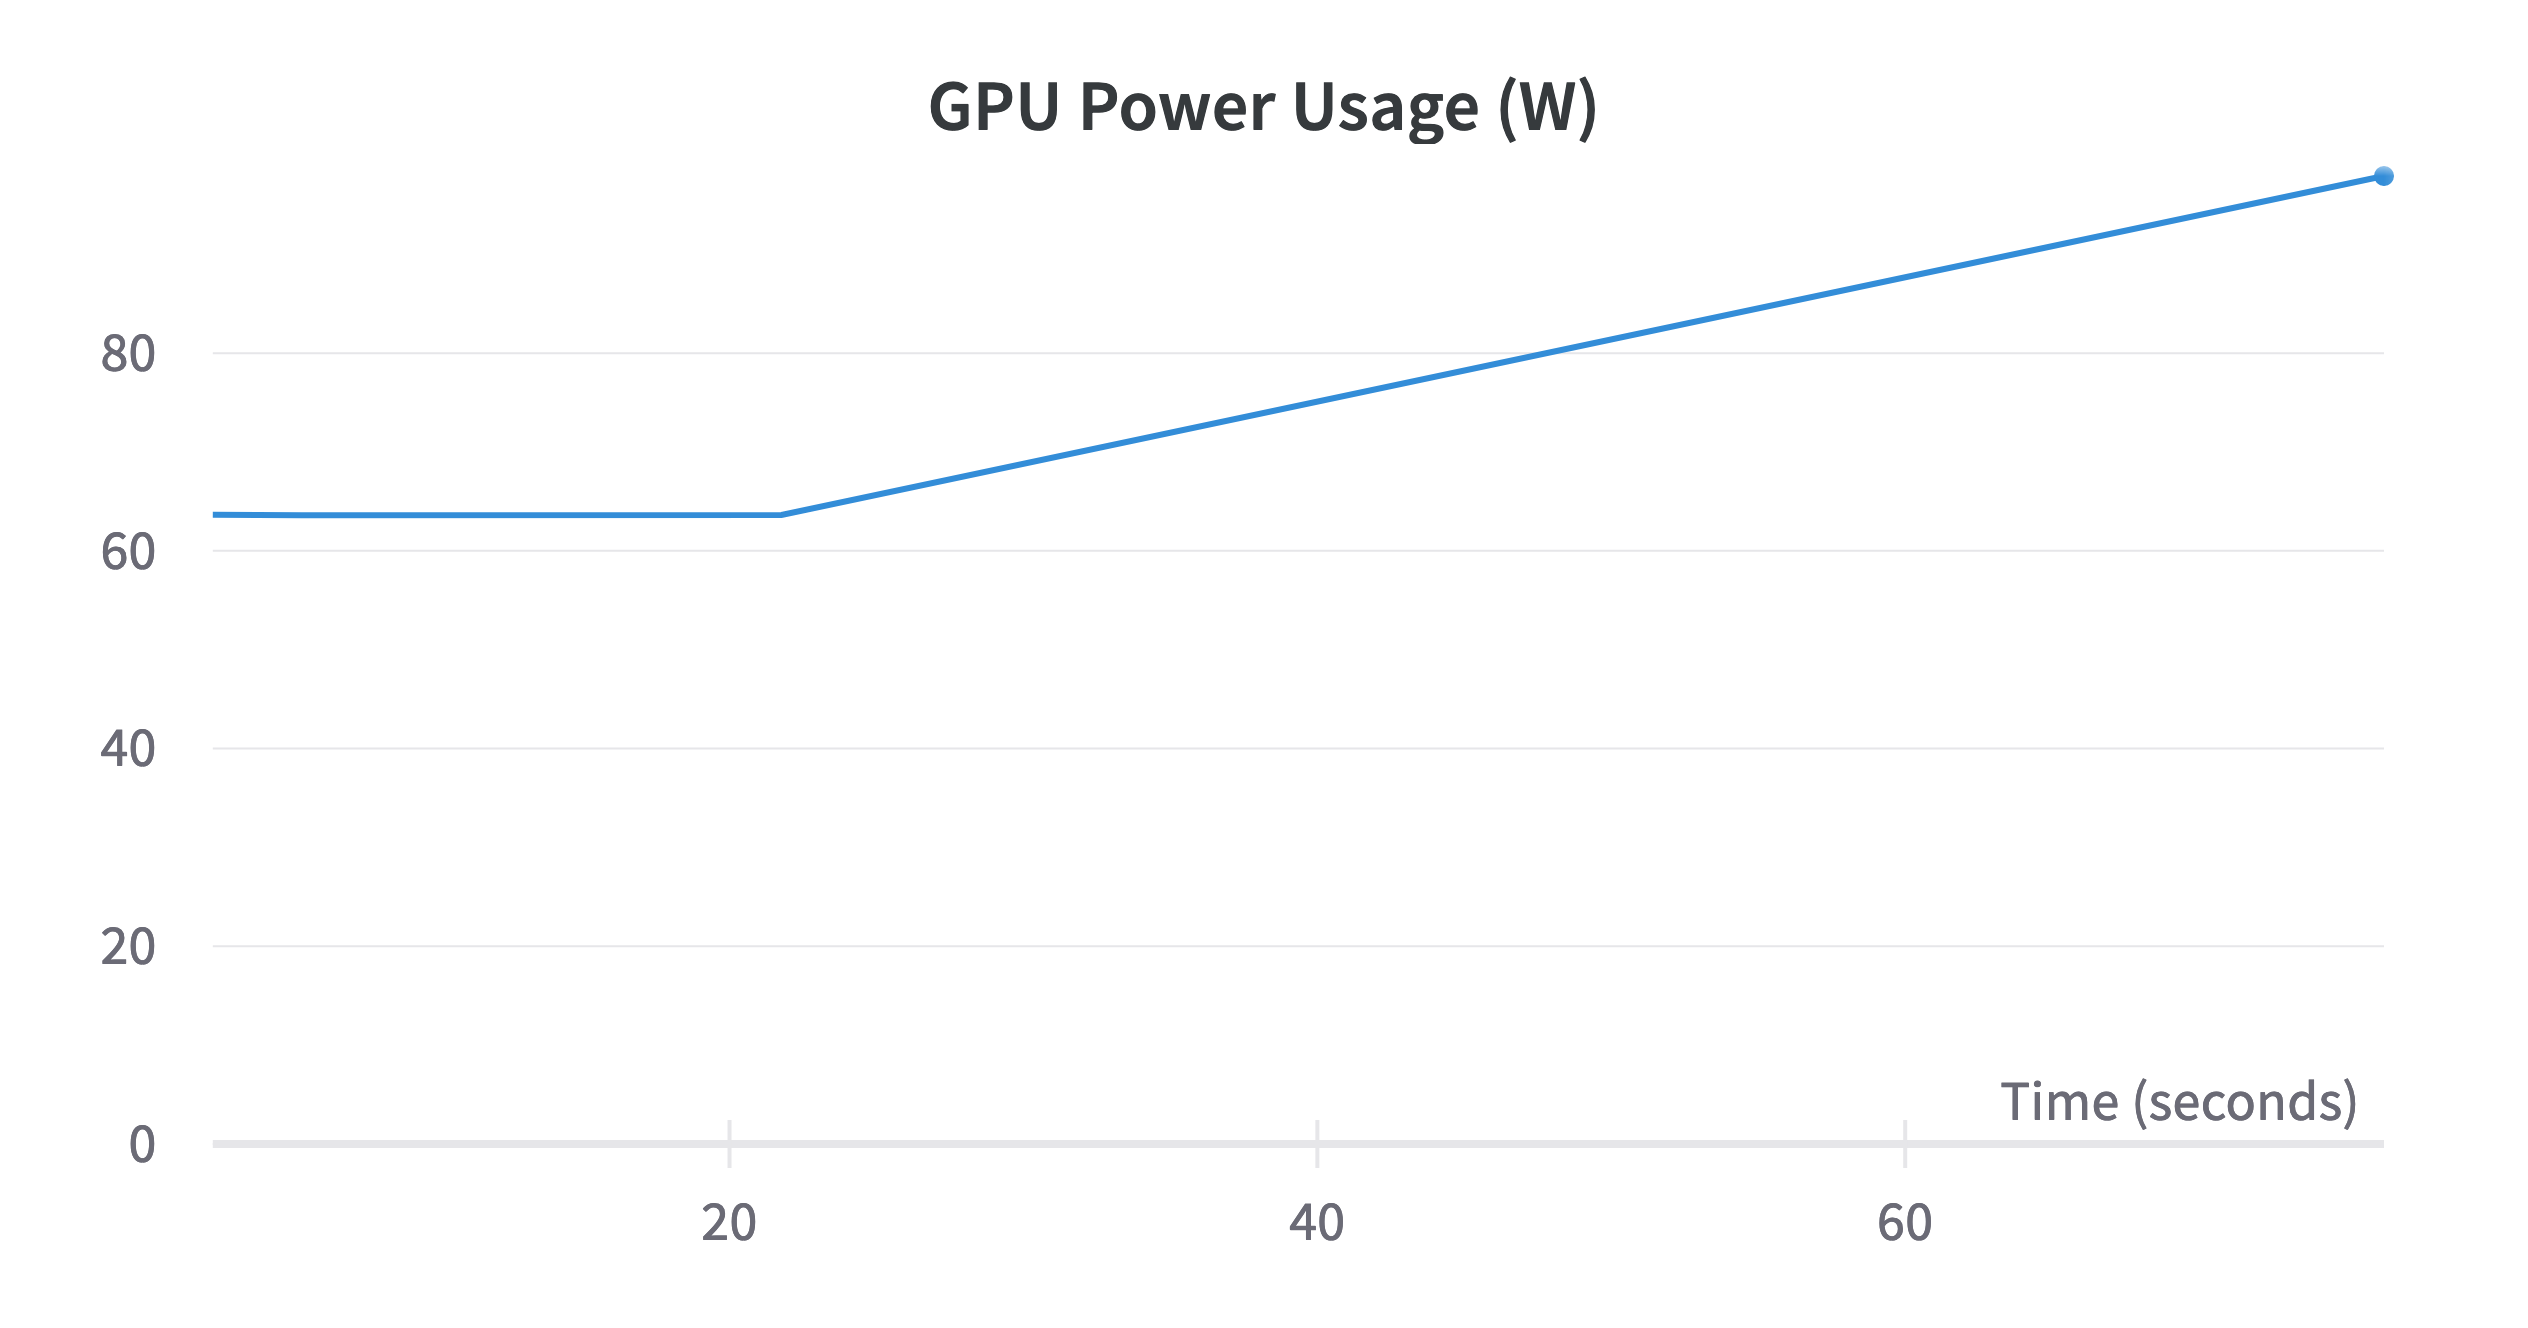
\includegraphics[width=\textwidth]{chapters/3_models/imgs/ufnc/ufncusagew.png}
	\end{subfigure}
	\begin{subfigure}{0.32\textwidth}
		\centering
		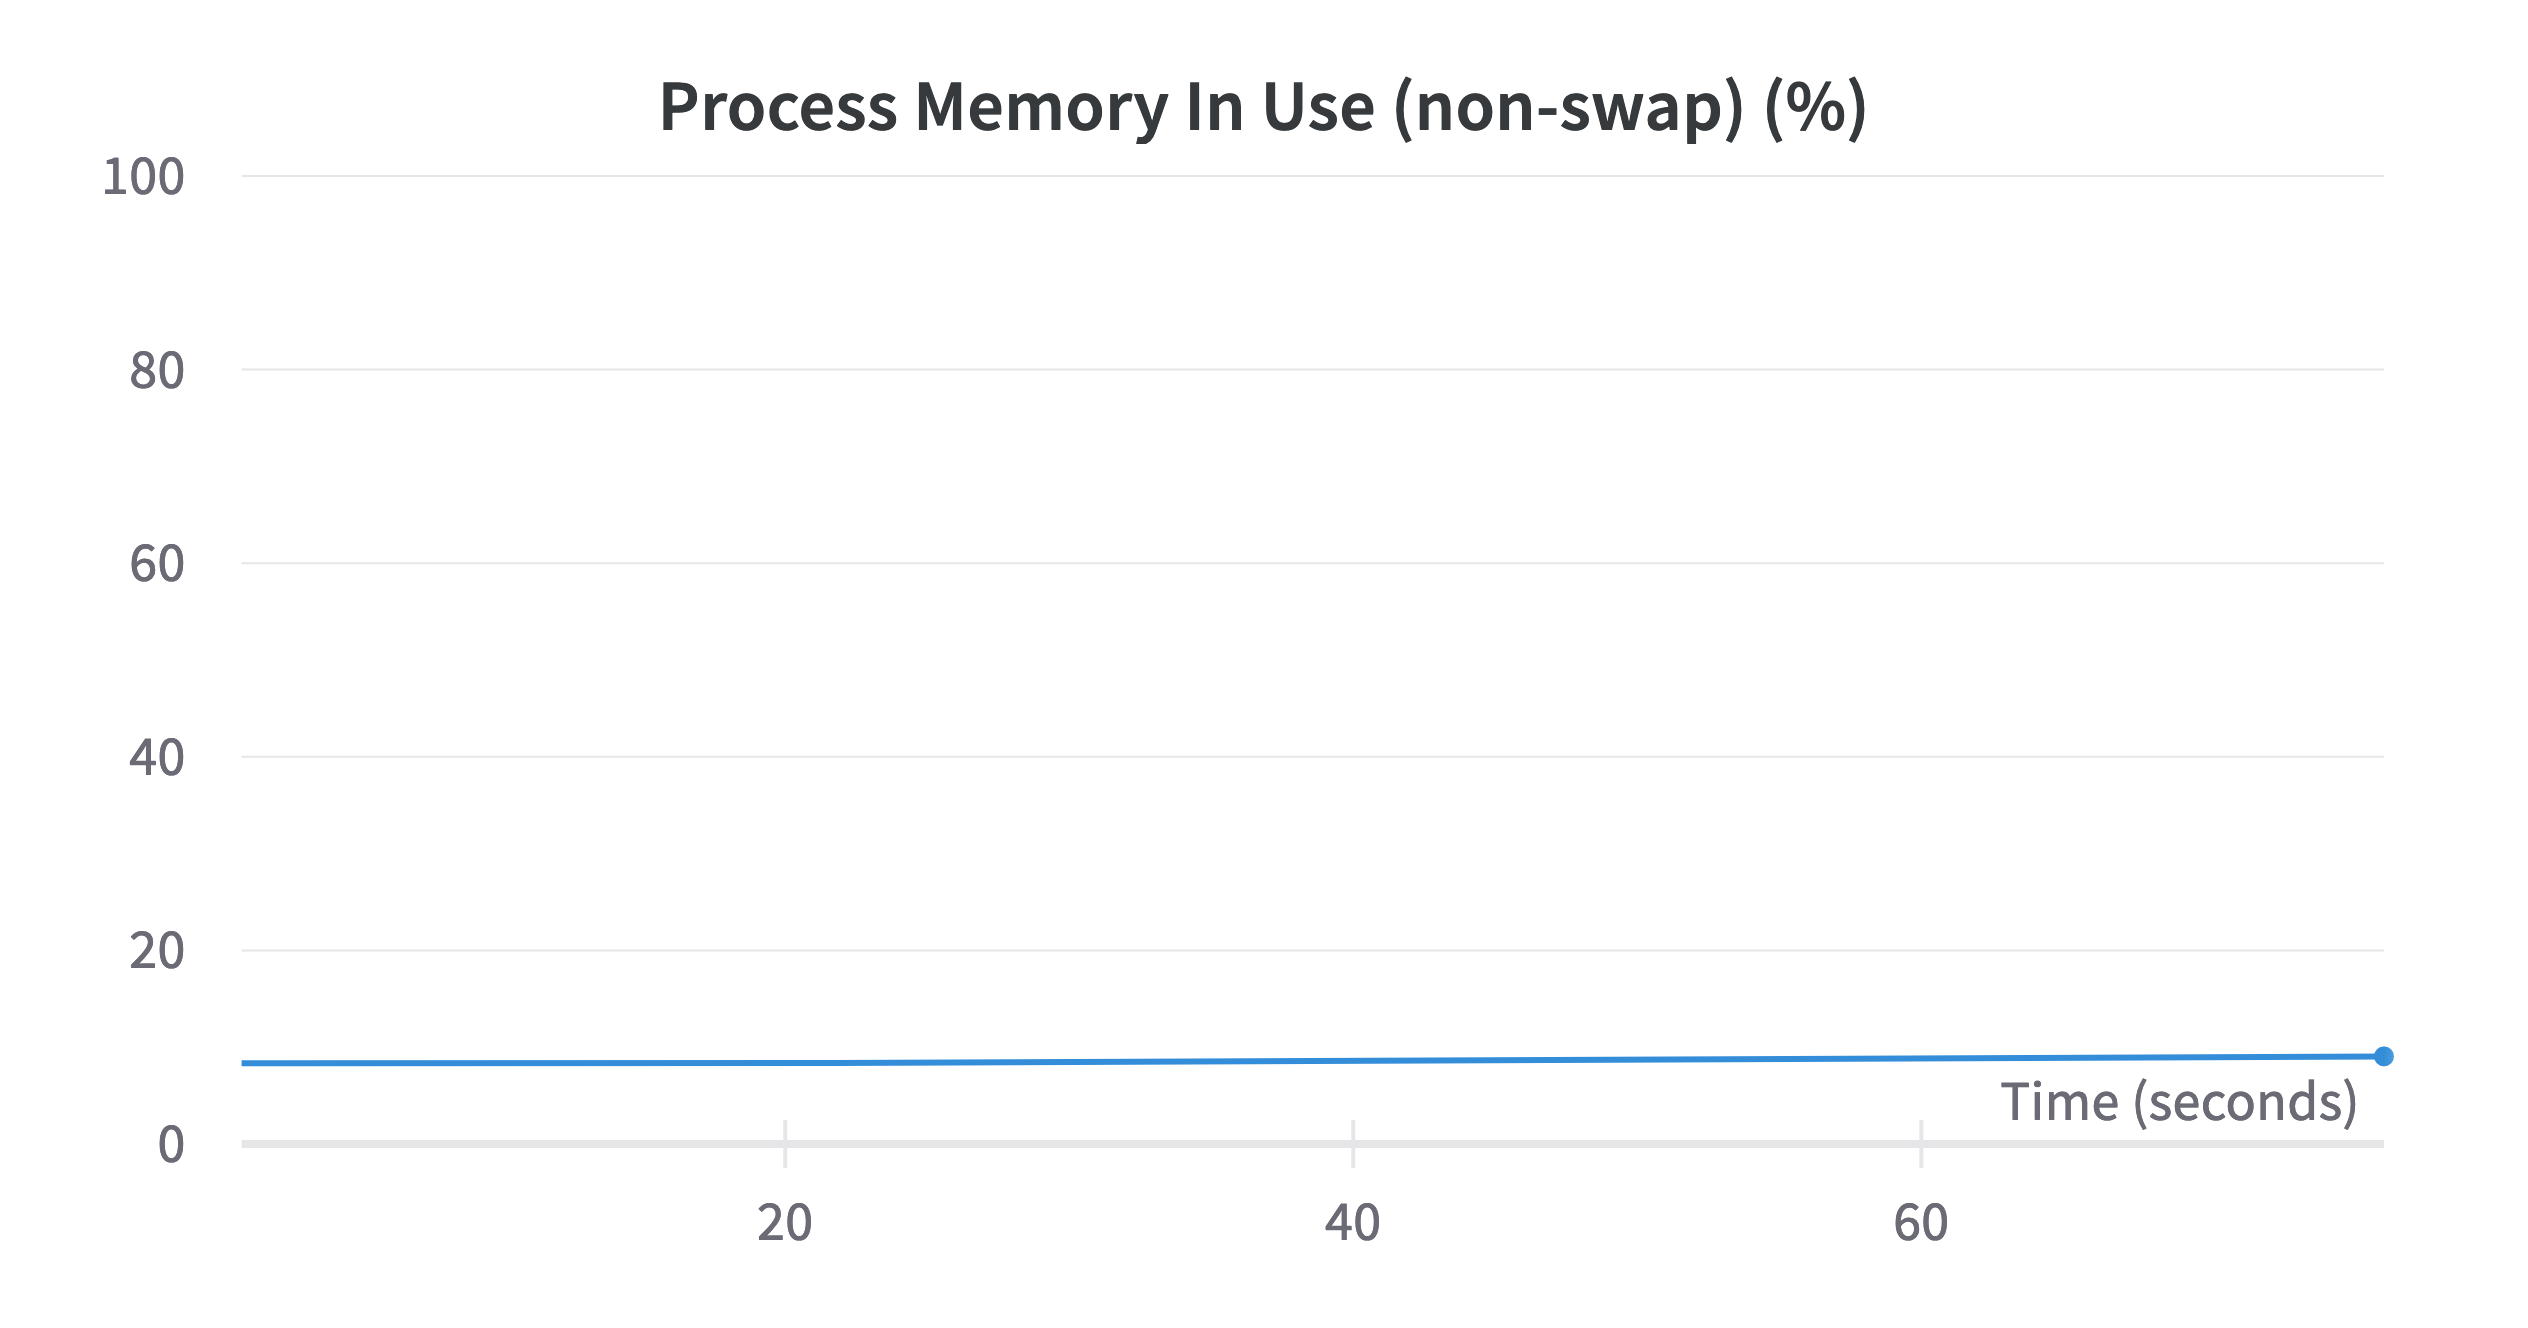
\includegraphics[width=\textwidth]{chapters/3_models/imgs/ufnc/ufcnmemram.png}
	\end{subfigure}\\
	\caption{System resources utilized during the Training phase.}
	\label{fig:ufcnsysusage}
\end{figure}

\begin{algorithm}[H]
	\caption{MLP model Training Algorithm}\label{alg:ufcntraining}
	\begin{algorithmic}
		\Require train/validation datasets; Baseline Neural Network Model

		\State Batch Size $\gets$ 10
		\State Learning Rate $\lambda \gets$ 0.01
		\State Epochs $\gets$ 100
		\State Patience $\gets$ 20
		\State loss $\gets$ L1Loss()
		\State Optimizer $\gets$ Adam Optimizer
		\State
		\For{\textbf{each} epoch \textbf{in} epochs}
		\For{\textbf{each} (batch\_id, before, after, target) \textbf{in} train.next\_batch()}

		\State train\_prediction $\gets$ model(before, after) \Comment{Model inference}
		\State train\_prediction $\gets \frac{\text{train\_prediction} \cdot \sum\text{train\_prediction}}{\sum target}$ \Comment{Area normalization}
		\State train\_loss $\gets$ loss(train\_prediction, target)
		\State Optimizer step
		\State Back Propagation
		\EndFor
		\State stop computing gradient
		\For{\textbf{each} (batch\_id, vbefore, vafter, vtarget) \textbf{in} validation.next\_batch()}
		\State val\_prediction $\gets$ model(vbefore, vafter) \Comment{Model inference}
		\State val\_prediction $\gets \frac{\text{val\_prediction} \cdot \sum\text{val\_prediction}}{\sum vtarget}$ \Comment{Area normalization}
		\State val\_loss $\gets$ loss(val\_prediction, vtarget)
		\EndFor

		\State check for Early Stopping
		\State check for Save Best Result
		\State start computing gradient
		\EndFor
	\end{algorithmic}
\end{algorithm}



\section{RNN based model Evaluation}
From the graphs shown in Figure~\ref{fig:grruntraining},
we can see that the training phase was successful,
and after an initial descent, the loss values remained relatively
constant without displaying any abnormal trends.
The statistics presented in Figure~\ref{fig:grrunsysusage} reveal
that the machine at our disposal was not fully utilized,
suggesting that this architecture can be trained and used on
less powerful computers than the one we have.
Additionally, the model appears to be very lightweight, both in terms
of the relatively small number of parameters and its weight,
which doesn't exceed 400~KB.


\begin{table}[H]
	\begin{center}
		\begin{tabular}[c]{l|l|l}
			%\cline{2-4}
			\multicolumn{1}{c|}{\textbf{Gap Period}} &
			\multicolumn{1}{c|}{\textbf{MAE (kW)}}   &
			\multicolumn{1}{c}{\textbf{R}$^2$}                     \\
			\hline

			02-04 to 05-04                           & 4.72 & 0.96 \\
			04-04 to 04-04                           & 3.60 & 0.93 \\
			12-04 to 14-04                           & 6.61 & 0.96
			% 06-04 to 07-04 & 20.07 & 0.62 &1293.53&50.70&1293.53&25.22 \\
		\end{tabular}
	\end{center}
	\caption{The table displays the values of MAE (Mean Absolute Error) and the R$^2$ (R-squared) index applied to the model predictions shown in Figures~\ref{fig:grrunevalplots}.}
	%La tabella mostra i valori del MAE e dell'indice R$^2$ applicate alle predizioni del modello mostrate nelle Figure~\ref{fig:ufcnevalbelli} e \ref{fig:ufcnevalbrutti}.}\label{tab:dfsplit}
\end{table}

\begin{table}[H]
	\begin{minipage}[t]{.45\textwidth}
		\begin{center}
			\begin{tabular}[c]{l|l|l}
				\multicolumn{3}{c}{\textbf{\textit{02-04 to 05-04 Gap}}}       \\
				%\hline
				               & \multicolumn{1}{c|}{\textbf{MAE (kW)}} &
				\multicolumn{1}{c}{\textbf{MAPE (\%)}}                         \\
				\hline
				\textbf{Day 1} & 97.03                                  & 1.99 \\
				\textbf{Day 2} & 28.68                                  & 3.22 \\
				\textbf{Day 3} & 69.79                                  & 4.79 \\
				\textbf{Day 4} & 41.65                                  & 1.98
			\end{tabular}
			%\caption{}
		\end{center}
	\end{minipage}%
	\hfill
	\begin{minipage}[t]{.45\textwidth}
		\begin{center}
			\begin{tabular}[c]{l|l|l}
				\multicolumn{3}{c}{\textbf{\textit{12-04 to 14-04 Gap}}}       \\
				%\hline
				               & \multicolumn{1}{c|}{\textbf{MAE (kW)}} &
				\multicolumn{1}{c}{\textbf{MAPE (\%)}}                         \\
				\hline
				\textbf{Day 1} & 151.93                                 & 2.86 \\
				\textbf{Day 2} & 49.44                                  & 1.01 \\
				\textbf{Day 3} & 111.25                                 & 2.76
			\end{tabular}
			%\caption{}
		\end{center}
	\end{minipage}%
	\vspace{1cm}
	\begin{minipage}{\textwidth}
		\begin{center}
			\begin{tabular}[c]{l|l|l}
				\multicolumn{3}{c}{\textbf{\textit{04-04 to 04-04 Gap}}}       \\
				%\hline
				               & \multicolumn{1}{c|}{\textbf{MAE (kW)}} &
				\multicolumn{1}{c}{\textbf{MAPE (\%)}}                         \\
				\hline
				\textbf{Day 1} & 0.93                                   & 0.06
			\end{tabular}
			%\caption{}
		\end{center}
	\end{minipage}
	\caption{The tables display the Daily MAE and MAPE values related to the graphs shown in Figure~\ref{fig:grrunevalplots}.}
	%Nelle tabelle sono mostrati i valori giornalieri di MAE e MAPE relativi ai grafici mostrati in Figura~\ref{fig:grrunevalplots}.}
\end{table}

%Dai grafici mostrati in Figura~\ref{fig:grruntraining} possiamo vedere come la fase di addestramento
%è andata a buon fine e, dopo una parte iniziale di discesa, i valori delle loss sono rimasti pressochè costanti e non mostrano andamenti anomali. Dalle statistiche riportate in Figura~\ref{fig:grrunsysusage} possiamo vedere come la macchina a nostra disposizione non è
%stata sfruttata a pieno e questo può portarci a pensare che questa architettura sia allenabile ed
%utilizzabile su computer meno perfromanti di quello a nostra disposizione. Inoltre il modello 
%risulta essere molto leggero, sia per il numero relativamente ridotto di parametri sia per il 
%peso che non supera i 400 KB.

\begin{figure}[H]
	\centering
	\begin{subfigure}{\textwidth}
		\centering
		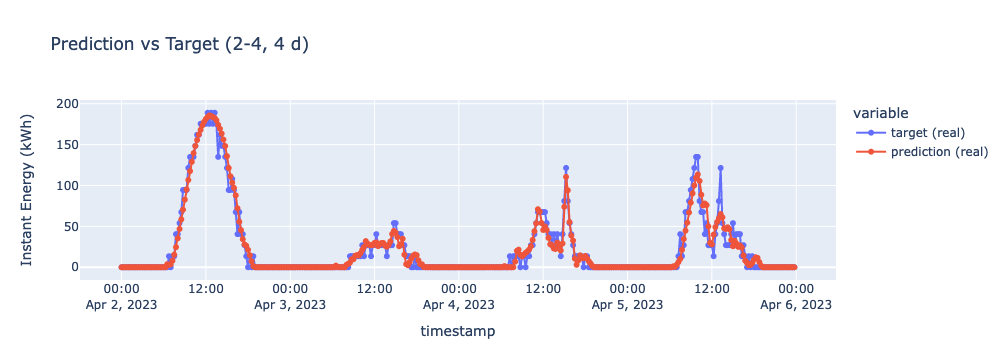
\includegraphics[width=\textwidth]{chapters/3_models/imgs/grrun/eval/grruneval24.png}
		\caption{}
	\end{subfigure}
	\begin{subfigure}{\textwidth}
		\centering
		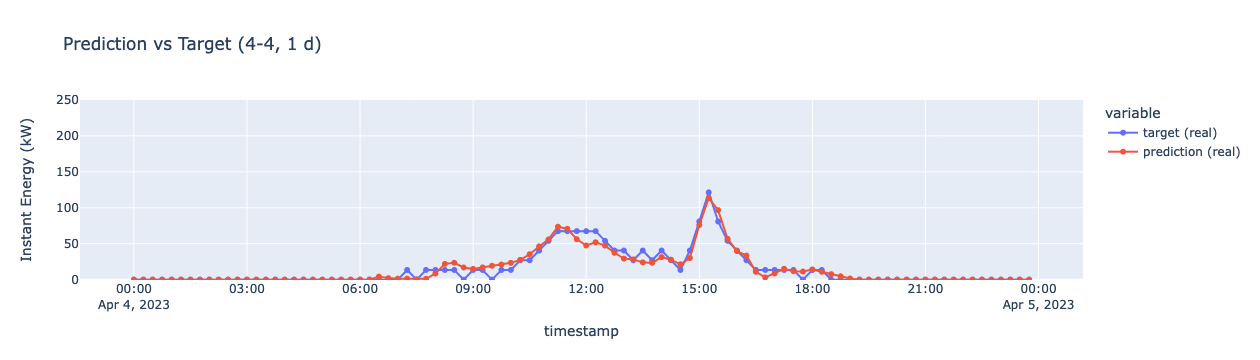
\includegraphics[width=\textwidth]{chapters/3_models/imgs/grrun/eval/grruneval44.png}
		\caption{}
	\end{subfigure}
	\begin{subfigure}{\textwidth}
		\centering
		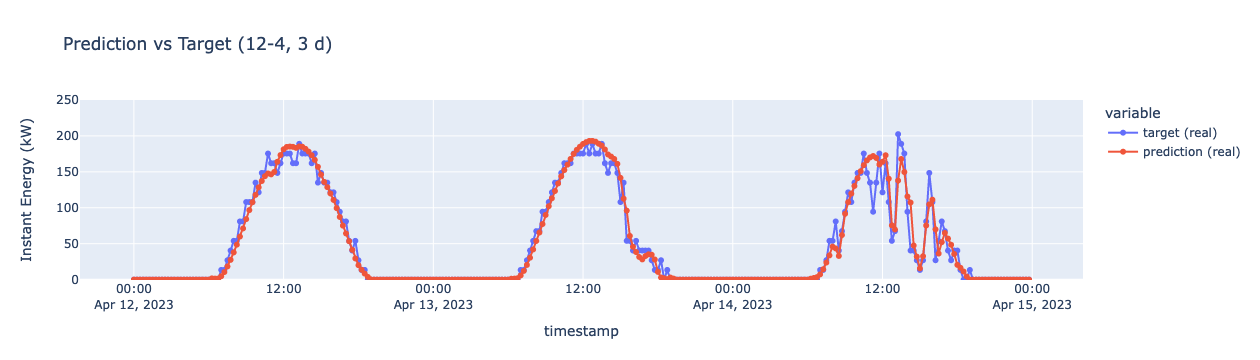
\includegraphics[width=\textwidth]{chapters/3_models/imgs/grrun/eval/grruneval124.png}
		\caption{}
	\end{subfigure}
	\caption{In the figure, three model predictions (in red) are shown alongside the ground truth (in blue) for gaps of varying sizes. These predictions were made using data from the testing dataset.}
	%In figura vengono mostrate 3 predizioni del modello (in rosso) comparate con la ground thorught (in blu) di buchi a dimensione variabile. Queste predizioni sono state effettuate con i dati provenienti dal dataset di Testing.}
	\label{fig:grrunevalplots}
\end{figure}
\newpage
Analyzing some model predictions as shown in
Figure~\ref{fig:grrunevalplots}, we can observe how the real
instant energy production curves (displayed in blue) are
closely approximated by the model (red curves).
The model effectively understands the plant's behavior,
even managing to predict production spikes.
We can also see that energy production is consistently zero during
the night in the predictions, and it adeptly captures the
day/night cycle by gradually reducing production as sunset approaches.

In graph (a), we can see a 4-day gap from 02-04-2023 to 06-04-2023.
The first two days are predicted very well, while in the last part,
we can see that a production spike was not detected.
In graph (b), we can observe a 1-day gap on 04-04-2023. We notice that the overall trend is almost entirely approximated correctly, except for some time intervals around 12:00.
The last graph (c) is related to a 3-day gap, and we can see that the first two days are approximated well, while in the last day, the production spikes are identified but with values not entirely similar to those of the ground truth.
%Analizzando alcune predizioni del modello riportate in Figura~\ref{fig:grrunevalplots} possiamo notare come le curve dell'energia 
%istantanea prodotta realmente (mostrate in blu) vengono approssimate decisamente
%bene dal modello (curve in rosso). Il modello riesce a capire bene il comportamento
%dell'impianto riuscendo anche a prevedere eventuali picchi di produzione.
%Possiamo notare come di notte la produzione di energia nelle predizioni è sempre nulla e come riesce molto bene a comprendere il ciclo giorno/notte
%andando ad azzerare gradualmente la produzione quando si avvicina il tramonto.

%Nel grafico (a) possiamo vedere un buco di 4 giorni che va dal 02-04-2023 al 06-04-2023. I primi due giorni vengono predetti molto bene, mentre nell'ultimo possiamo vedere che un picco di produzione non è stato individuato.
%Nel prolt (b) possiamo apprezzare un buco di 1 giorno, il 04-04-2023.
%Notiamo come l'andamento è quasi del tutto approsiamoto correttamente tranne
%che per alcuni intervalli temporali che si aggirano intorno le 12:00.
%L'ultimo grafico (c) è relativo ad un buco di 3 giorni e possiamo vedere
%come i primi due vengono approssimati bene, mentre nell'ultimo i picchi
%di produzione vengono si individuati ma con valori non del tutto simili
%a quelli della ground truth.

\begin{figure}[H]
	\centering
	\begin{subfigure}{\textwidth}
		\centering
		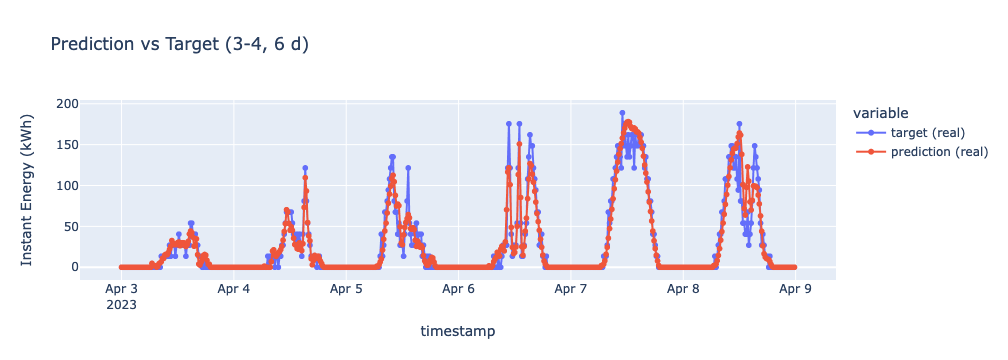
\includegraphics[width=.9\textwidth]{chapters/3_models/imgs/grrun/eval/grruneval6buco.png}
		\caption{}
	\end{subfigure}
	\begin{subfigure}{\textwidth}
		\centering
		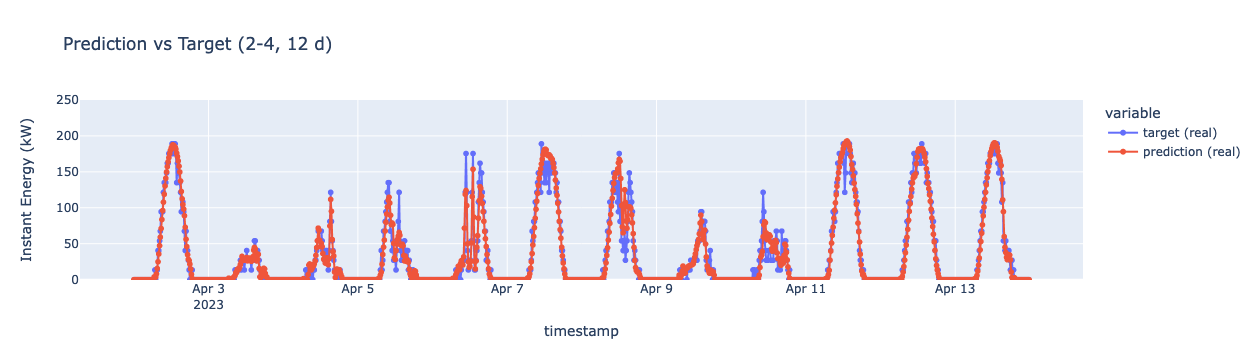
\includegraphics[width=.9\textwidth]{chapters/3_models/imgs/grrun/eval/grruneval12buco.png}
		\caption{}
	\end{subfigure}
	\caption{The graphs depict two model predictions for gaps that exceed the maximum limit of days set during the training phase. The first one (a) shows a 6-day gap, while the second one (b) presents a 12-day gap.}
	%I grafici mostrano due predizioni del modello di buchi con dimensioni che superano il limite massimo di giorni impostati nella fase di training. Il primo (a) mostra un buco di 6 giorni, mentre il secondo (b) uno di 12.}
	\label{fig:grrunevalbucogrande}
\end{figure}

It is interesting to note how the model still performs well even
when presented with gaps that exceed the maximum length set
during training.
In Figure~\ref{fig:grrunevalbucogrande}, two graphs are shown:
(a) represents a 6-day gap (two days longer than the maximum length),
and (b) a 12-day gap.
Given these results, we can conclude that the model can
generalize effectively and predict instant energy production
trends with considerable reliability.


%\'{E} interessante notare come il modello riesce a perforare comunque bene anche se gli vengono passati dei buchi che superano la dimensione massima impostata durante l'addestramento. In Figura~\ref{fig:grrunevalbucogrande} vengono mostrati due grafici, (a) è un buco di 6 giorni (due in più della dimensione massima), mentre (b) è di 12. Dati questi risultati possiamo
%affermare che il modello è in grado di generalizzare molto bene e riuscire
%a predirre l'andamento dell'energia istantanea prodotta con notevole affidabilità.

\begin{table}[H]
	\begin{minipage}[t]{.45\textwidth}
		\begin{center}
			\begin{tabular}[c]{l|l|l}
				\multicolumn{3}{c}{\textbf{\textit{03-04 to 08-04 Gap}}}       \\
				%\hline
				               & \multicolumn{1}{c|}{\textbf{MAE (kW)}} &
				\multicolumn{1}{c}{\textbf{MAPE (\%)}}                         \\
				\hline
				\textbf{Day 1} & 151.93                                 & 2.86 \\
				\textbf{Day 2} & 49.44                                  & 1.01 \\
				\textbf{Day 3} & 111.25                                 & 2.76 \\
				\textbf{Day 4} & 0.93                                   & 0.06 \\
				\textbf{Day 5} & 0.93                                   & 0.06 \\
				\textbf{Day 6} & 0.93                                   & 0.06
			\end{tabular}
			%\caption{}
		\end{center}
	\end{minipage}%
	\hfill
	\begin{minipage}[t]{.45\textwidth}
		\begin{center}
			\begin{tabular}[c]{l|l|l}
				\multicolumn{3}{c}{\textbf{\textit{02-04 to 13-04 Gap}}}        \\
				%\hline
				                & \multicolumn{1}{c|}{\textbf{MAE (kW)}} &
				\multicolumn{1}{c}{\textbf{MAPE (\%)}}                          \\
				\hline
				\textbf{Day 1}  & 148.45                                 & 3.04 \\
				\textbf{Day 2}  & 38.14                                  & 4.28 \\
				\textbf{Day 3}  & 55.41                                  & 3.80 \\
				\textbf{Day 4}  & 20.26                                  & 0.96 \\
				\textbf{Day 5}  & 104.28                                 & 4.09 \\
				\textbf{Day 6}  & 112.09                                 & 2.18 \\
				\textbf{Day 7}  & 312.26                                 & 8.79 \\
				\textbf{Day 8}  & 47.65                                  & 3.46 \\
				\textbf{Day 9}  & 16.32                                  & 0.99 \\
				\textbf{Day 10} & 23.08                                  & 0.43 \\
				\textbf{Day 11} & 240.66                                 & 4.52 \\
				\textbf{Day 12} & 22.21                                  & 0.45
			\end{tabular}
			%\caption{}
		\end{center}
	\end{minipage}
	\caption{The tables presented refer to the graphs in Figure~\ref{fig:grrunevalbucogrande} and display the corresponding Daily MAE and MAPE metrics.}
	%Le tabelle mostrate fanno riferimento ai grafici in Figura~\ref{fig:grrunevalbucogrande} e mostrano le relative metriche Daily MAE e MAPE.}
	%Nelle tabelle sono mostrati i valori giornalieri di MAE e MAPE relativi ai grafici mostrati in Figura~\ref{fig:grrunevalplots}.}
\end{table}
\section{Transformers}\label{sec:gab}
Now, we will introduce a third model with an architecture based on Transformers\cite{attention}.
We will analyze its layers, the training phase, highlighting the differences
compared to the previous ones, especially in the construction of the input.
%We will see how this model will prove to be the best among the three models presented in this thesis.

%Ora introdurremo un terzo modello la cui architettura di basa sui 
%Transformers. Andremo ad analizzare la sua architettura, la
%fase di traning evidenziando le differenze rispetto alle precedenti
%soprattutto nella costruzione dell'input e vedremo come questo risulterà 
%essere il migliore tra i tre modelli presentati in questa tesi.

\subsection{Architecture}
The input and operation of this model are slightly different
from what we have seen previously.
This model requires only one tensor as input, representing the data for an entire week, with the \verb|target| feature containing a variable period of values set to \textquote{-1}. This special character, called \textit{placeholder}, indicates to the model the presence of a gap that needs to be filled. %{\bf (*VP* dire meglio che l'input è uno solo invece di più tensori come negli altri modelli, e che il -1 è un placeholder che indica i dati mancanti, se ho capito bene. )}
This gap can have an extremely variable length,
ranging from a minimum of 2 timestamps to the equivalent
of one-third of a week, and it can be positioned anywhere within the week.
This is a very interesting aspect of the model, as it allows it not only to detect the presence of gaps and fill them easily but also enables the immediate construction and preparation of the input.
%Questo è un aspetto molto interessante del modello che gli permette, oltre di poter individuare la presenza dei buchi e di chiuderli in modo semplice, permette anche una costruzione e preparazione immediata dell'input.
%{\bf (*VP* aggiungi una frasetta per dire che questa è una caratteristica interessante del modello che ne permette una applicabilità più ampia, più generale. Sempre se ho capito bene.)}

The model's objective is to learn to predict the entire week, including the gap.
Through a masking system, we can then extract only the values of interest.
Let's now delve into the specific elements that characterize and make up this model:


%L'input ed il funzionamento di questo modello è leggermente differente
%da quelli che abbiamo visto in precedenza. Questo necessita di
%un'intera settimana in input con al suo interno un buco che viene
%rappresentato da una sequenza di caratteri speciali, nello specifico \textquote{-1}. Questo buco potrà avere una lunghezza estremamente variabile:
%da un minimo di 2 timestamp fino all'equivalente di un terzo di settimana
%e potrà essere posizionato ovunque all'interno di questa.
%Il modello avrà quindi l'obbiettivo di apprendere a predirre 
%tutta la settimana, compreso il buco, e tramite un sistema di maschere
%saremmo in grado poi di poter estrapolare solo i valori di nostro
%interesse.
%
%Analizziamo ora nel dettaglio i principali elementi che caratterizzano e compongono questo modello:

\begin{itemize}
	\item \textbf{Input}: As described earlier,
	      the input is a tensor containing one week of data with the
	      target feature that includes a period of -1 (representing the gap).
	\item \textbf{Convolution}: The input goes through two convolutional layers to extract and understand the most important and representative features of the time series. Each layer undergoes batch normalization, and the Gaussian Error Linear Units (GELU)\cite{gelu} function is used as the activation function.
	\item \textbf{Positional Encoder}: To help the model understand the temporal sequence and the order of the different time series, a positional encoder called Time Absolute Position Encoding (tAPE)\cite{tape} is implemented. It incorporates the series length and input embedding dimension for absolute position encoding\cite{tape}.
	\item \textbf{Transformer Encoder}: After performing positional encoding on the output of the convolutional layers, it is passed to the transformer. This transformer\cite{attention} consists of 2 transformer layers, each of which contains 8 heads for multi-head attention\cite{attention}, 64 layers for the feed-forward part, a dropout rate of 0.1, and GELU as the activation function.
	\item \textbf{Output}: This is the final layer of the network, responsible for reshaping the transformer's output to the required dimension for use. It is a feed-forward layer with an output dimension of 1, and it applies the Softplus\cite{functions} function as the activation function.
\end{itemize}

%\begin{itemize}
%    \item \textbf{Input}: come descritto prima, un tensore contenente
%    sempre 1 settimana di dati con all'interno la feature target che presenta un periodo con valori di -1 (buco).
%    \item \textbf{Convoluzione}: l'input viene passatro attraverso
%    due livelli Convolutivi per cercare di ottenere e comprendere
%    le feature più importanti e rappresentative della serie.
%    Ad ognuno di questi viene applicata una procedura di Batch
%    Normaization ed impiegata la Gaussian Error Linear Units (GELU) come funzione di attivazione.
%    \item \textbf{Positional Encoder}: per peremttere al modello
%    di comprendere la successione del tempo e l'ordinamento
%    delle varie serie temporali abbiamo implementato il positional encoder time Absolute Position Encoding (tAPE), il quale incorporates 
%    the series length and input embedding dimension in absolute
%    position encoding.
%    \item \textbf{Transformer Encoder}: una volta effettuato il positional
%    encoding dell'output dei layer convolutivi, questo viene passato
%    al transformer. Questo è formato da 2 Transformers Layer ed ognuno
%    di questi è composto da 8 heads per la multiheadattention, 64 layer per la parte Feed Forward, 0.1 come valore
%    di dropout e la GELU come activation function.
%    \item \textbf{Output}: è l'ultimo livello della rete e si occupa di
%    riportare la dimensione dell'output del Transformer a quella necessaria
%    per poter essere utilizzata. \'{E} un layer feed forward con la dimensione dell'output pari a 1 e viene applicata la Softplus come
%    funzione di attivazione.
%\end{itemize}

\begin{figure}[H]
	\centering
	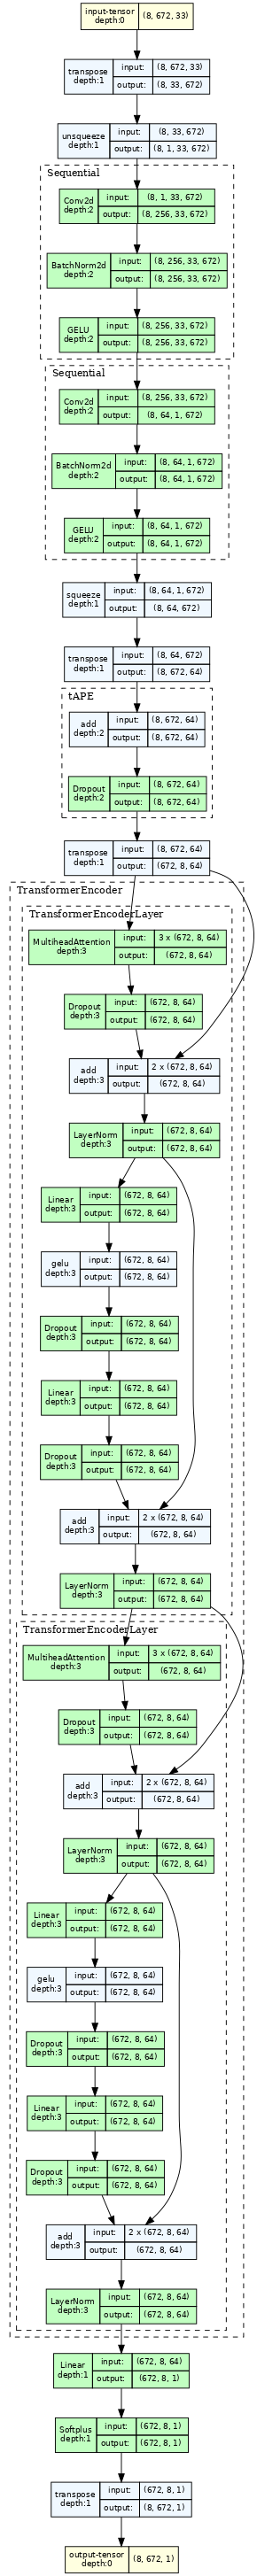
\includegraphics[height=\textheight]{chapters/3_models/imgs/gab/transformerarchitecture.png}
	\caption{Transformer Based Model architecture visualization.}\label{fig:gabarchitecture}
\end{figure}

\subsection{Training}
The model was trained using the input format discussed earlier,
generating gaps artificially in the training dataset, while also ensuring the
creation of a gap mask.
This mask is an array of the same length as the input time series,
composed of two elements: 1 to indicate the gap timestamps and 0 for regular timestamps.
This allows obtaining only the predicted values within the gap,
which are used for evaluating the loss function.

In this case, a procedure for normalizing the area was applied to ensure that the
model learns the gap curve's behavior.
The L1Loss (Equation~\ref{eq:l1loss}) function was employed as the loss function, and AdamW\cite{adamw} was used as the
optimizer with a learning rate ($\lambda$) set to 0.00001.
The learning rate is then adjusted during training using a cosine annealing scheduler\cite{scheduler1}\cite{scheduler2}
to provide optimal conditions for the model during this phase.

Additionally, a validation dataset was used to assess the model's
performance during training and to enable the
\textit{Early Stopping} and \textit{Save Best} procedures,
which were also used in this case.

	{\bf (*VP* valgono anche qui tutte le cose dette prima. Sarebbe opportuno giustificare la forma dei grafici reltaivi all'uso dlle risorse, visto che hanno una forma diversa (a trapezio) rispetto a quelle precedenti. Ovviamente se sai giustificarlo, altrimenti lascia stare.)}

%Il modello è stato allenato utilizzando il formato di input discusso in
%precedenza andando a creare buchi in modo artificiale nel dataset
%di training facendo attenzione a generare anche una maschera del buco: un
%array di lunghezza pari a quella della serie passata in input e coposto da due elementi, 1 indica i timestamp del buco mentre 0 quelli ordinari.
%In questo modo sarà possibile andare ad ottenere solo i valori del buco
%predetti dal modello per poi valutare la loss function solo su questi valori.
%Anche in questo caso è stata applicata una procedura di normalizzazione dell'area
%per assicurarci che il modello impari ad apprendere l'andamendo della curva
%del buco. E' stata impiegata la L1Loss come loss function, AdamW come
%optimizer con learning rate $\lambda$ pari a 0.00001 che poi 
%verrà variato durante la procedura di training tramite un cosine annealing scheduler per permettere al modello le migliori condizioni durante questa
%fase.
%Anche in questo caso è stato impiegato il dataset di validation per andare
%a misurare le performance del modello durante l'allenamento e per permettere
%il funzionamento delle procedure 
%\textit{Early Stopping} e \textit{Save Bast} che anche inquesto caso 
%sono state implementate.

\begin{table}[H]
	\begin{center}
		\begin{tabular}[c]{l|l}
			\textbf{Total Parameters (\#)}     & 594177 \\
			\textbf{Trainable Parameters (\#)} & 594177 \\
			\textbf{Training Duration (s)}     & 900.0  \\
			\textbf{Model Size (MB)}           & 2.4
		\end{tabular}
	\end{center}
	\caption{Transformer based model specification.}\label{tab:gabspecs}
\end{table}

\begin{figure}[H]
	\centering
	\begin{tikzpicture}
		\draw[->] (-3,0) -- (3,0) node[right] {$x$};
		\draw[->] (0,-1) -- (0,2) node[above] {$y$};
		\draw[dotted] (-3,-1) grid (3,2);
		\draw[color=blue, domain=-3:2] plot[id=logistic] function{0.5 * x * (1+tanh(sqrt(2/pi) * (x + 0.044715*x**3)))};
	\end{tikzpicture}
	\caption{Gaussian Error Linear Units (GELU). $GELU(x) = x * \Phi(x)$}
	\label{fig:gelu}
\end{figure}

\begin{figure}[H]
	\centering
	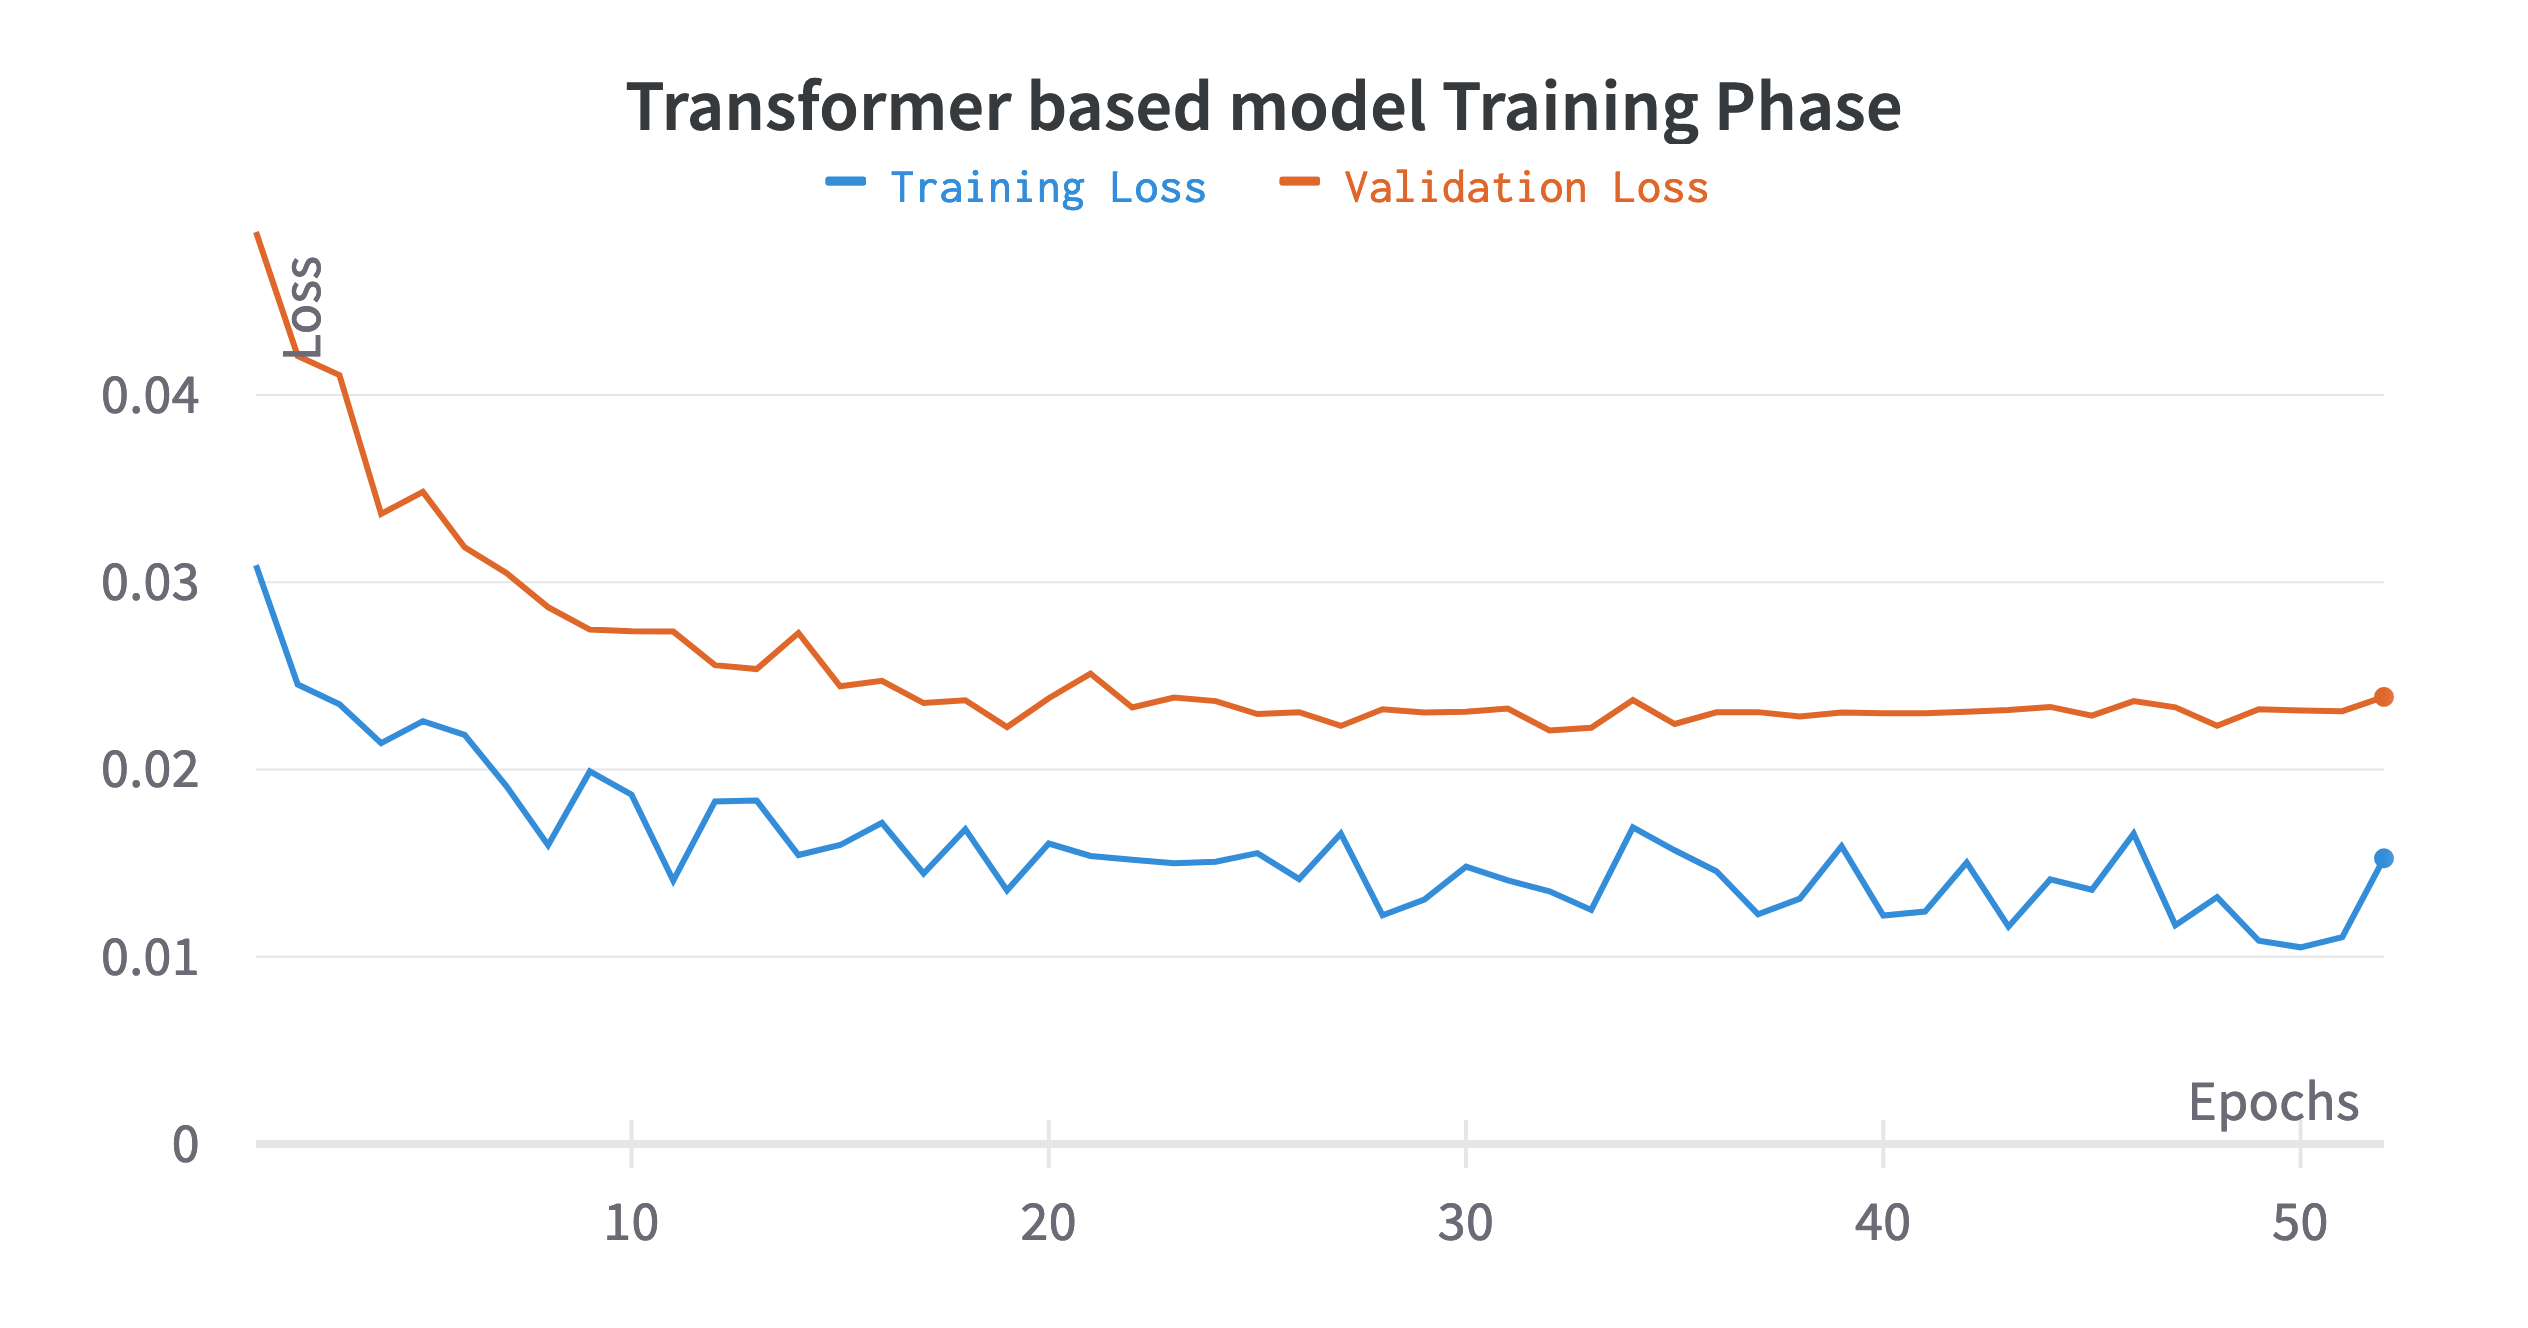
\includegraphics[width=.9\textwidth]{chapters/3_models/imgs/gab/gabtraining.png}
	\caption{The chart displays the loss progression during the training phase.The blue line represents the Training Loss, while the orange line represents the Validation Loss.}
	\label{fig:gabtrainchart}
\end{figure}

\begin{figure}[H]
	\centering
	\begin{subfigure}{0.43\textwidth}
		\centering
		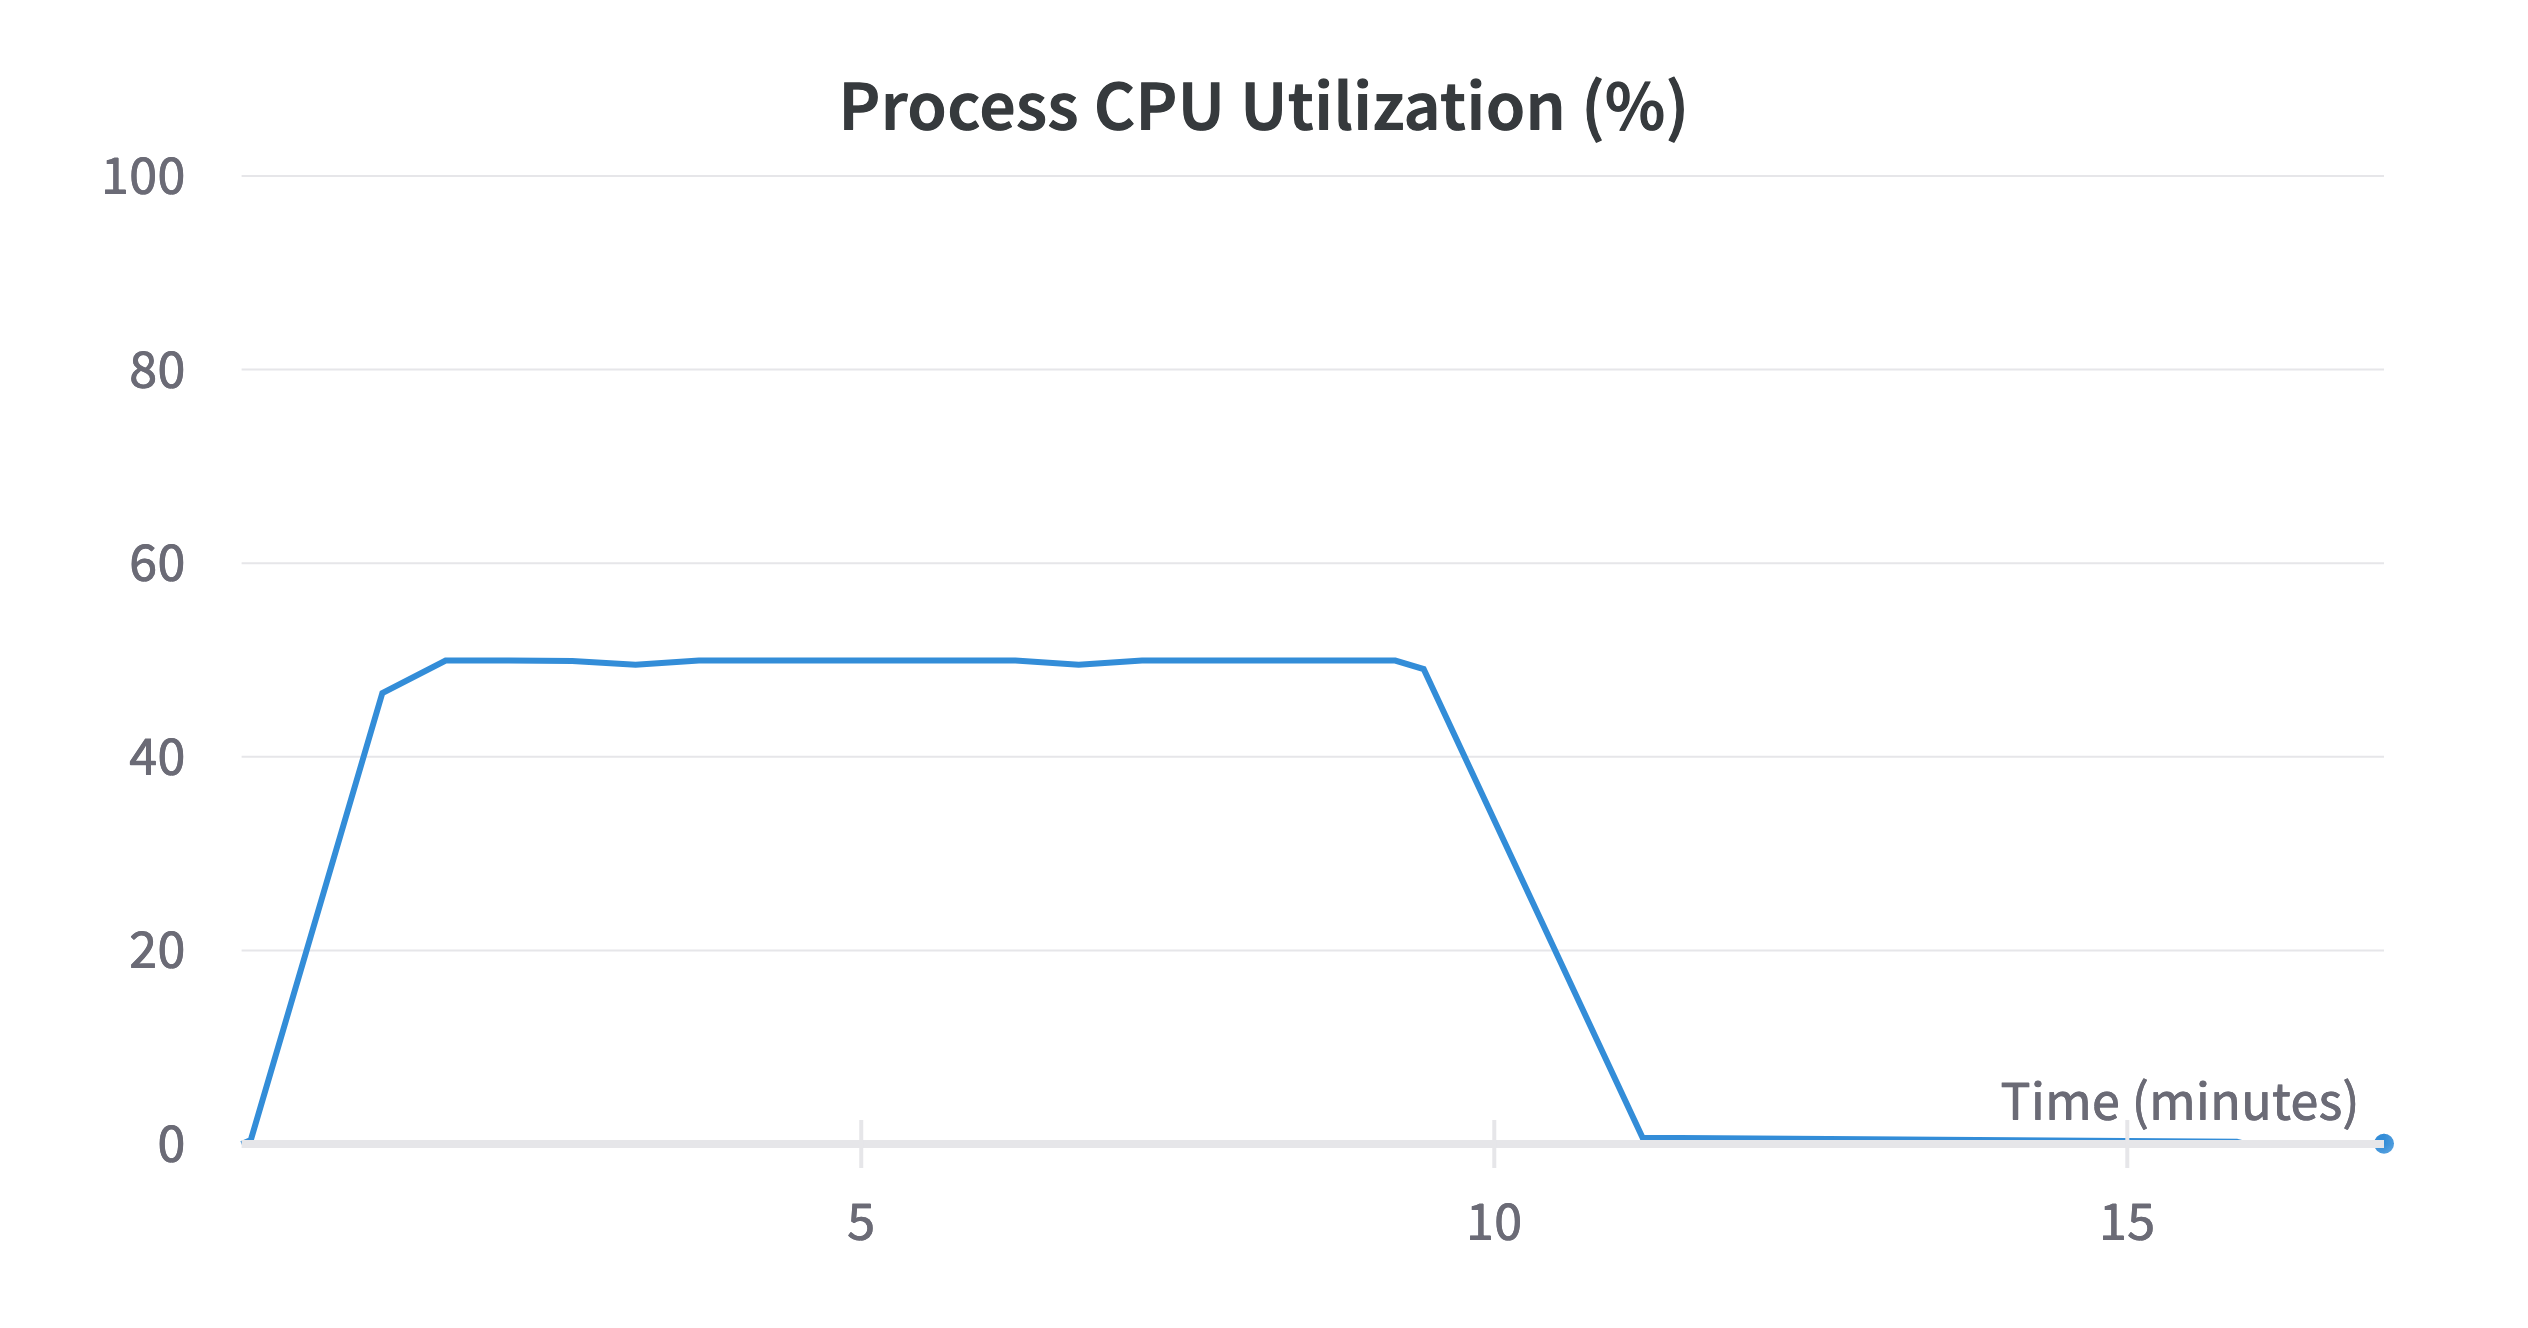
\includegraphics[width=\textwidth]{chapters/3_models/imgs/gab/train/gabrielcputilization.png}
	\end{subfigure}
	\begin{subfigure}{0.43\textwidth}
		\centering
		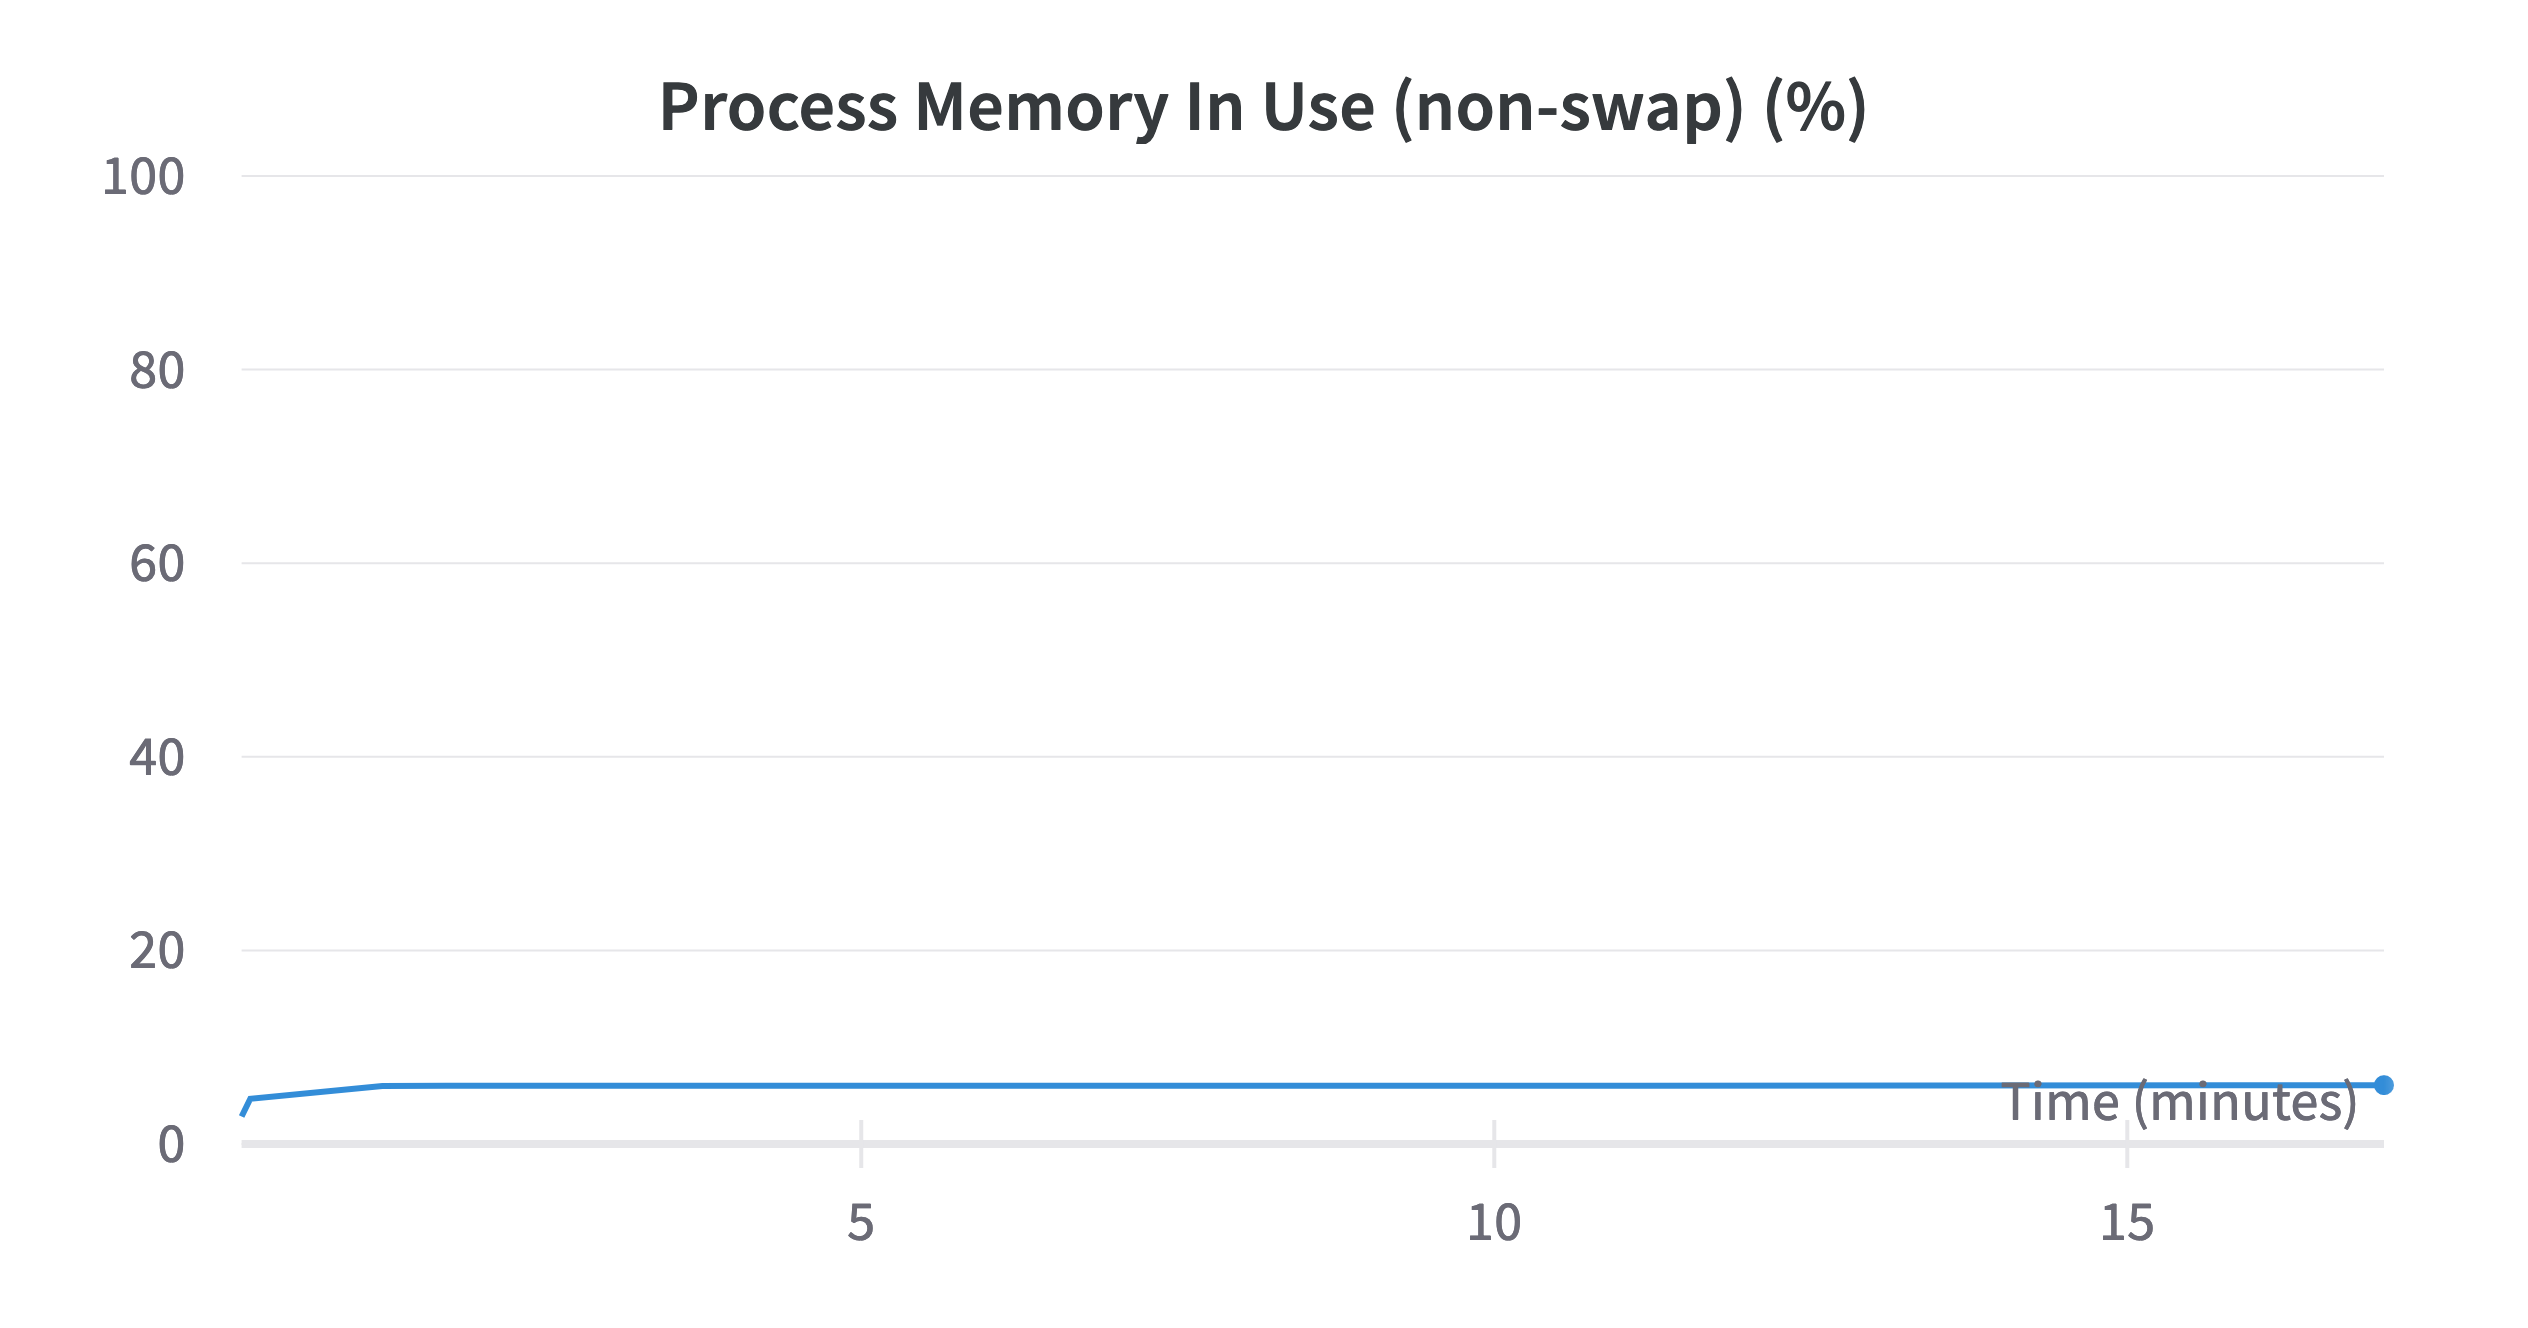
\includegraphics[width=\textwidth]{chapters/3_models/imgs/gab/train/gabrielprocessmemory.png}
	\end{subfigure}\\
	\begin{subfigure}{0.43\textwidth}
		\centering
		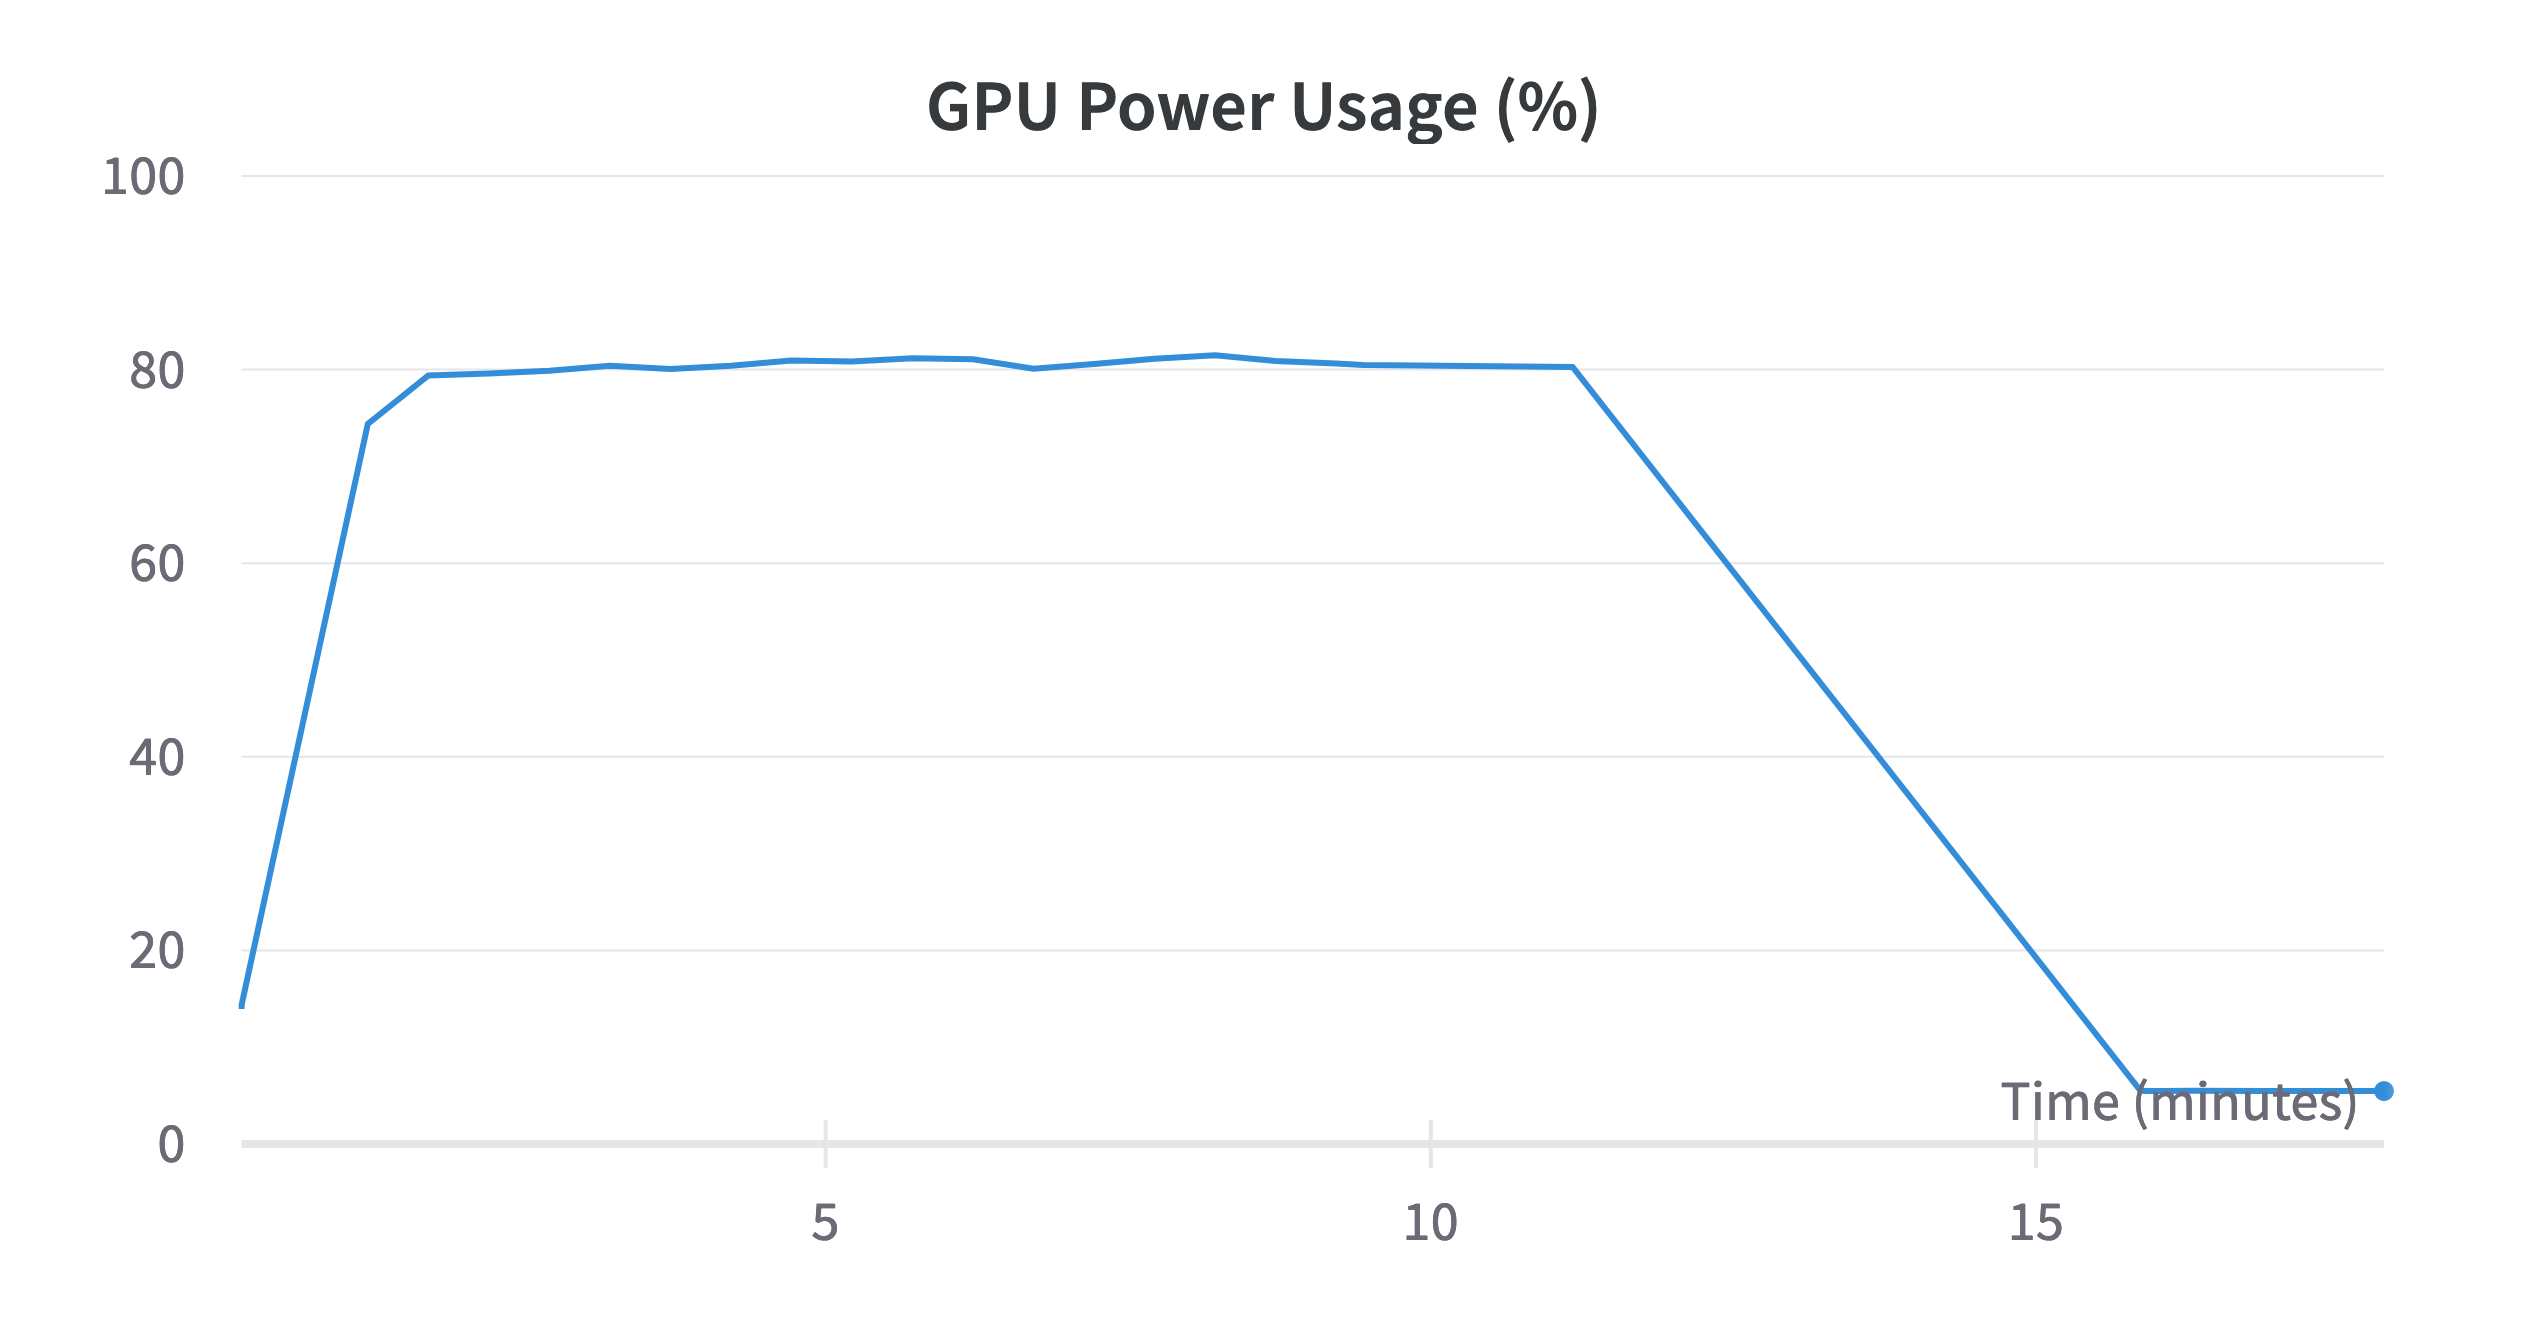
\includegraphics[width=\textwidth]{chapters/3_models/imgs/gab/train/gabrielgpupowerusageperc.png}
	\end{subfigure}
	\begin{subfigure}{0.43\textwidth}
		\centering
		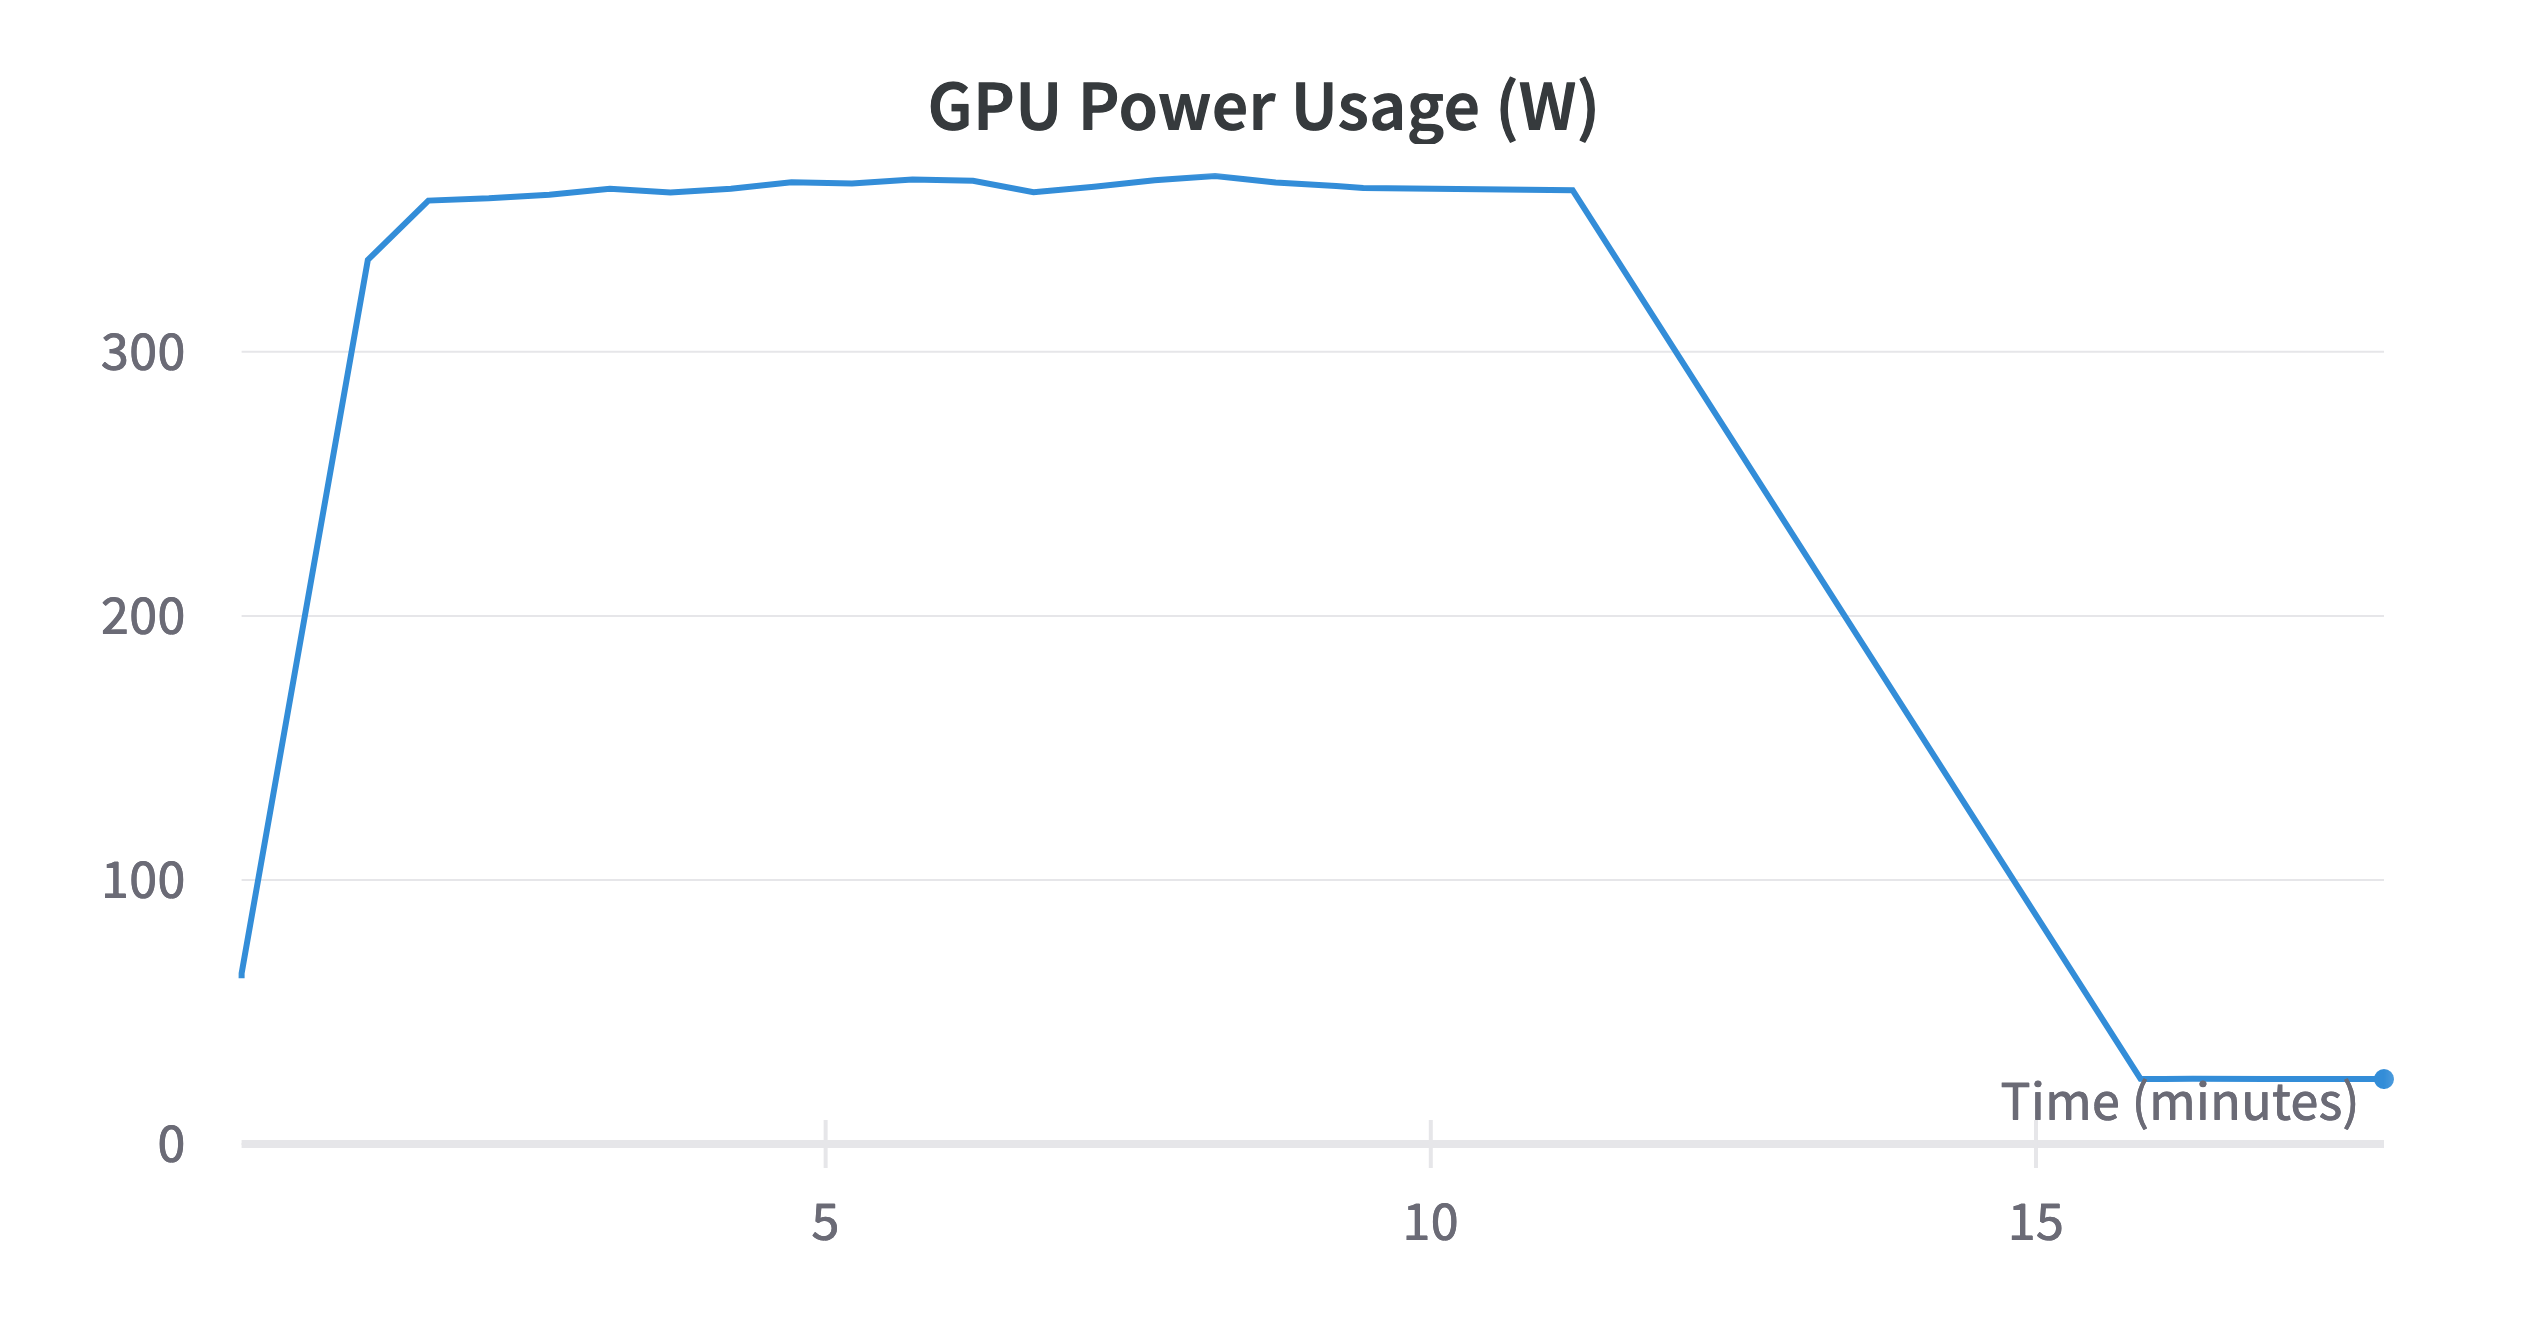
\includegraphics[width=\textwidth]{chapters/3_models/imgs/gab/train/gabrielgpupowerusagew.png}
	\end{subfigure}\\
	\begin{subfigure}{0.43\textwidth}
		\centering
		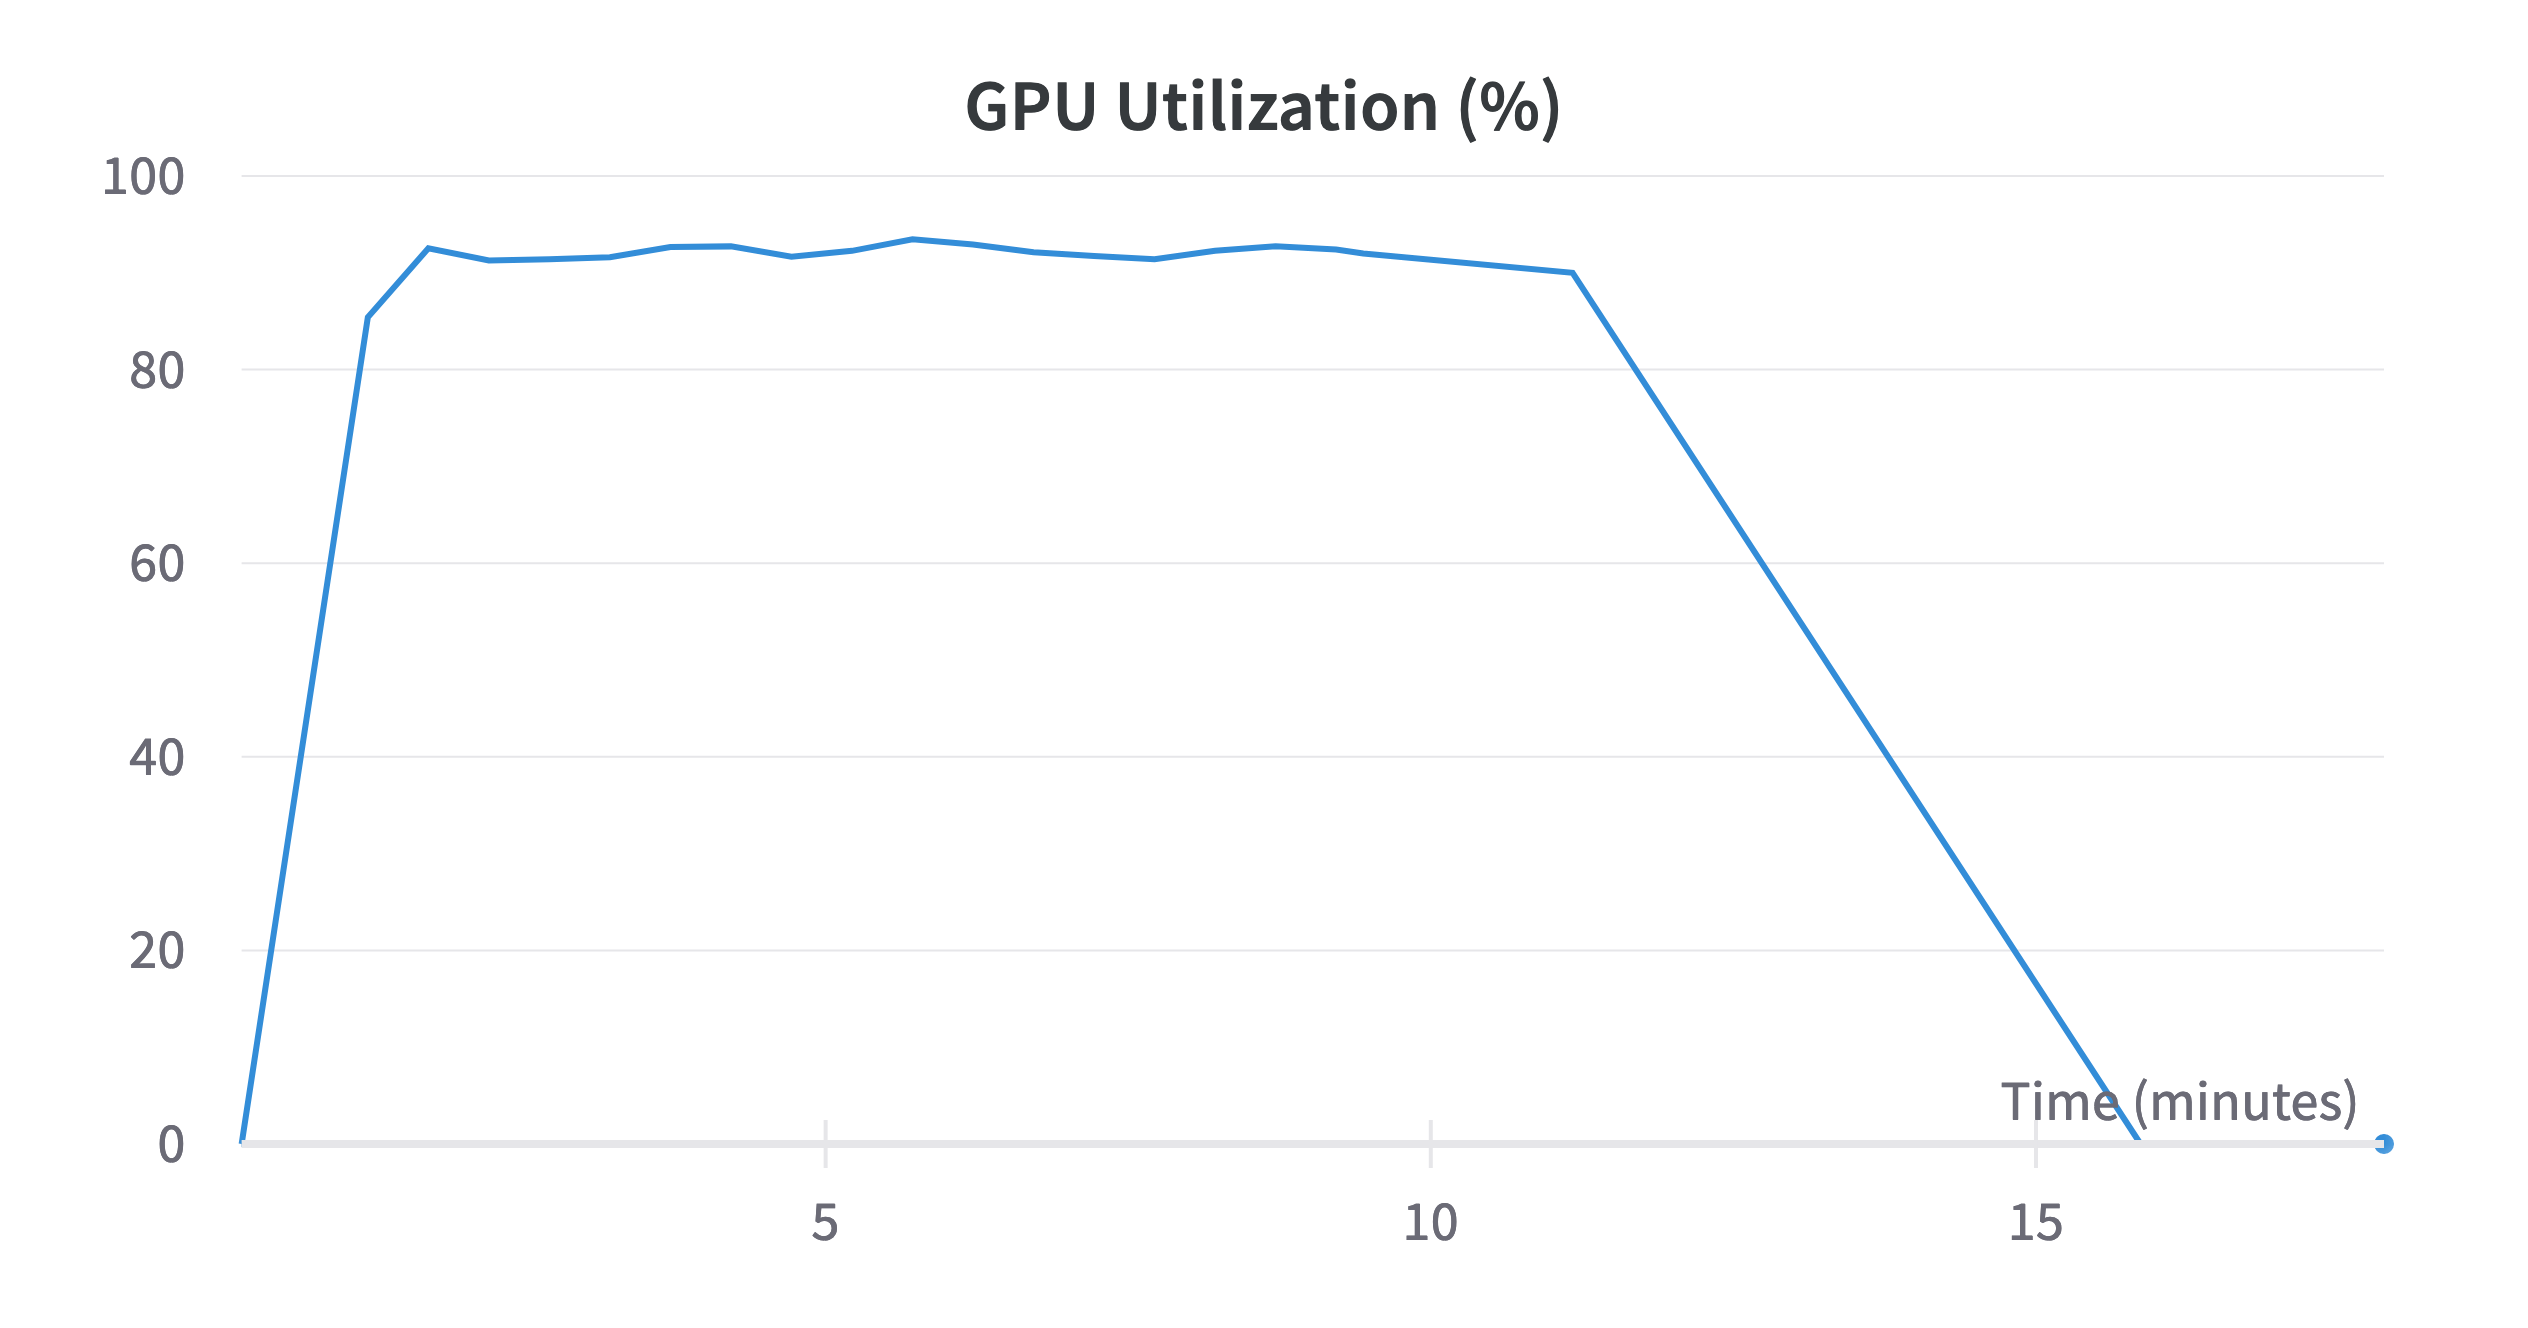
\includegraphics[width=\textwidth]{chapters/3_models/imgs/gab/train/gabrielgpuutilizationperc.png}
	\end{subfigure}
	\begin{subfigure}{0.43\textwidth}
		\centering
		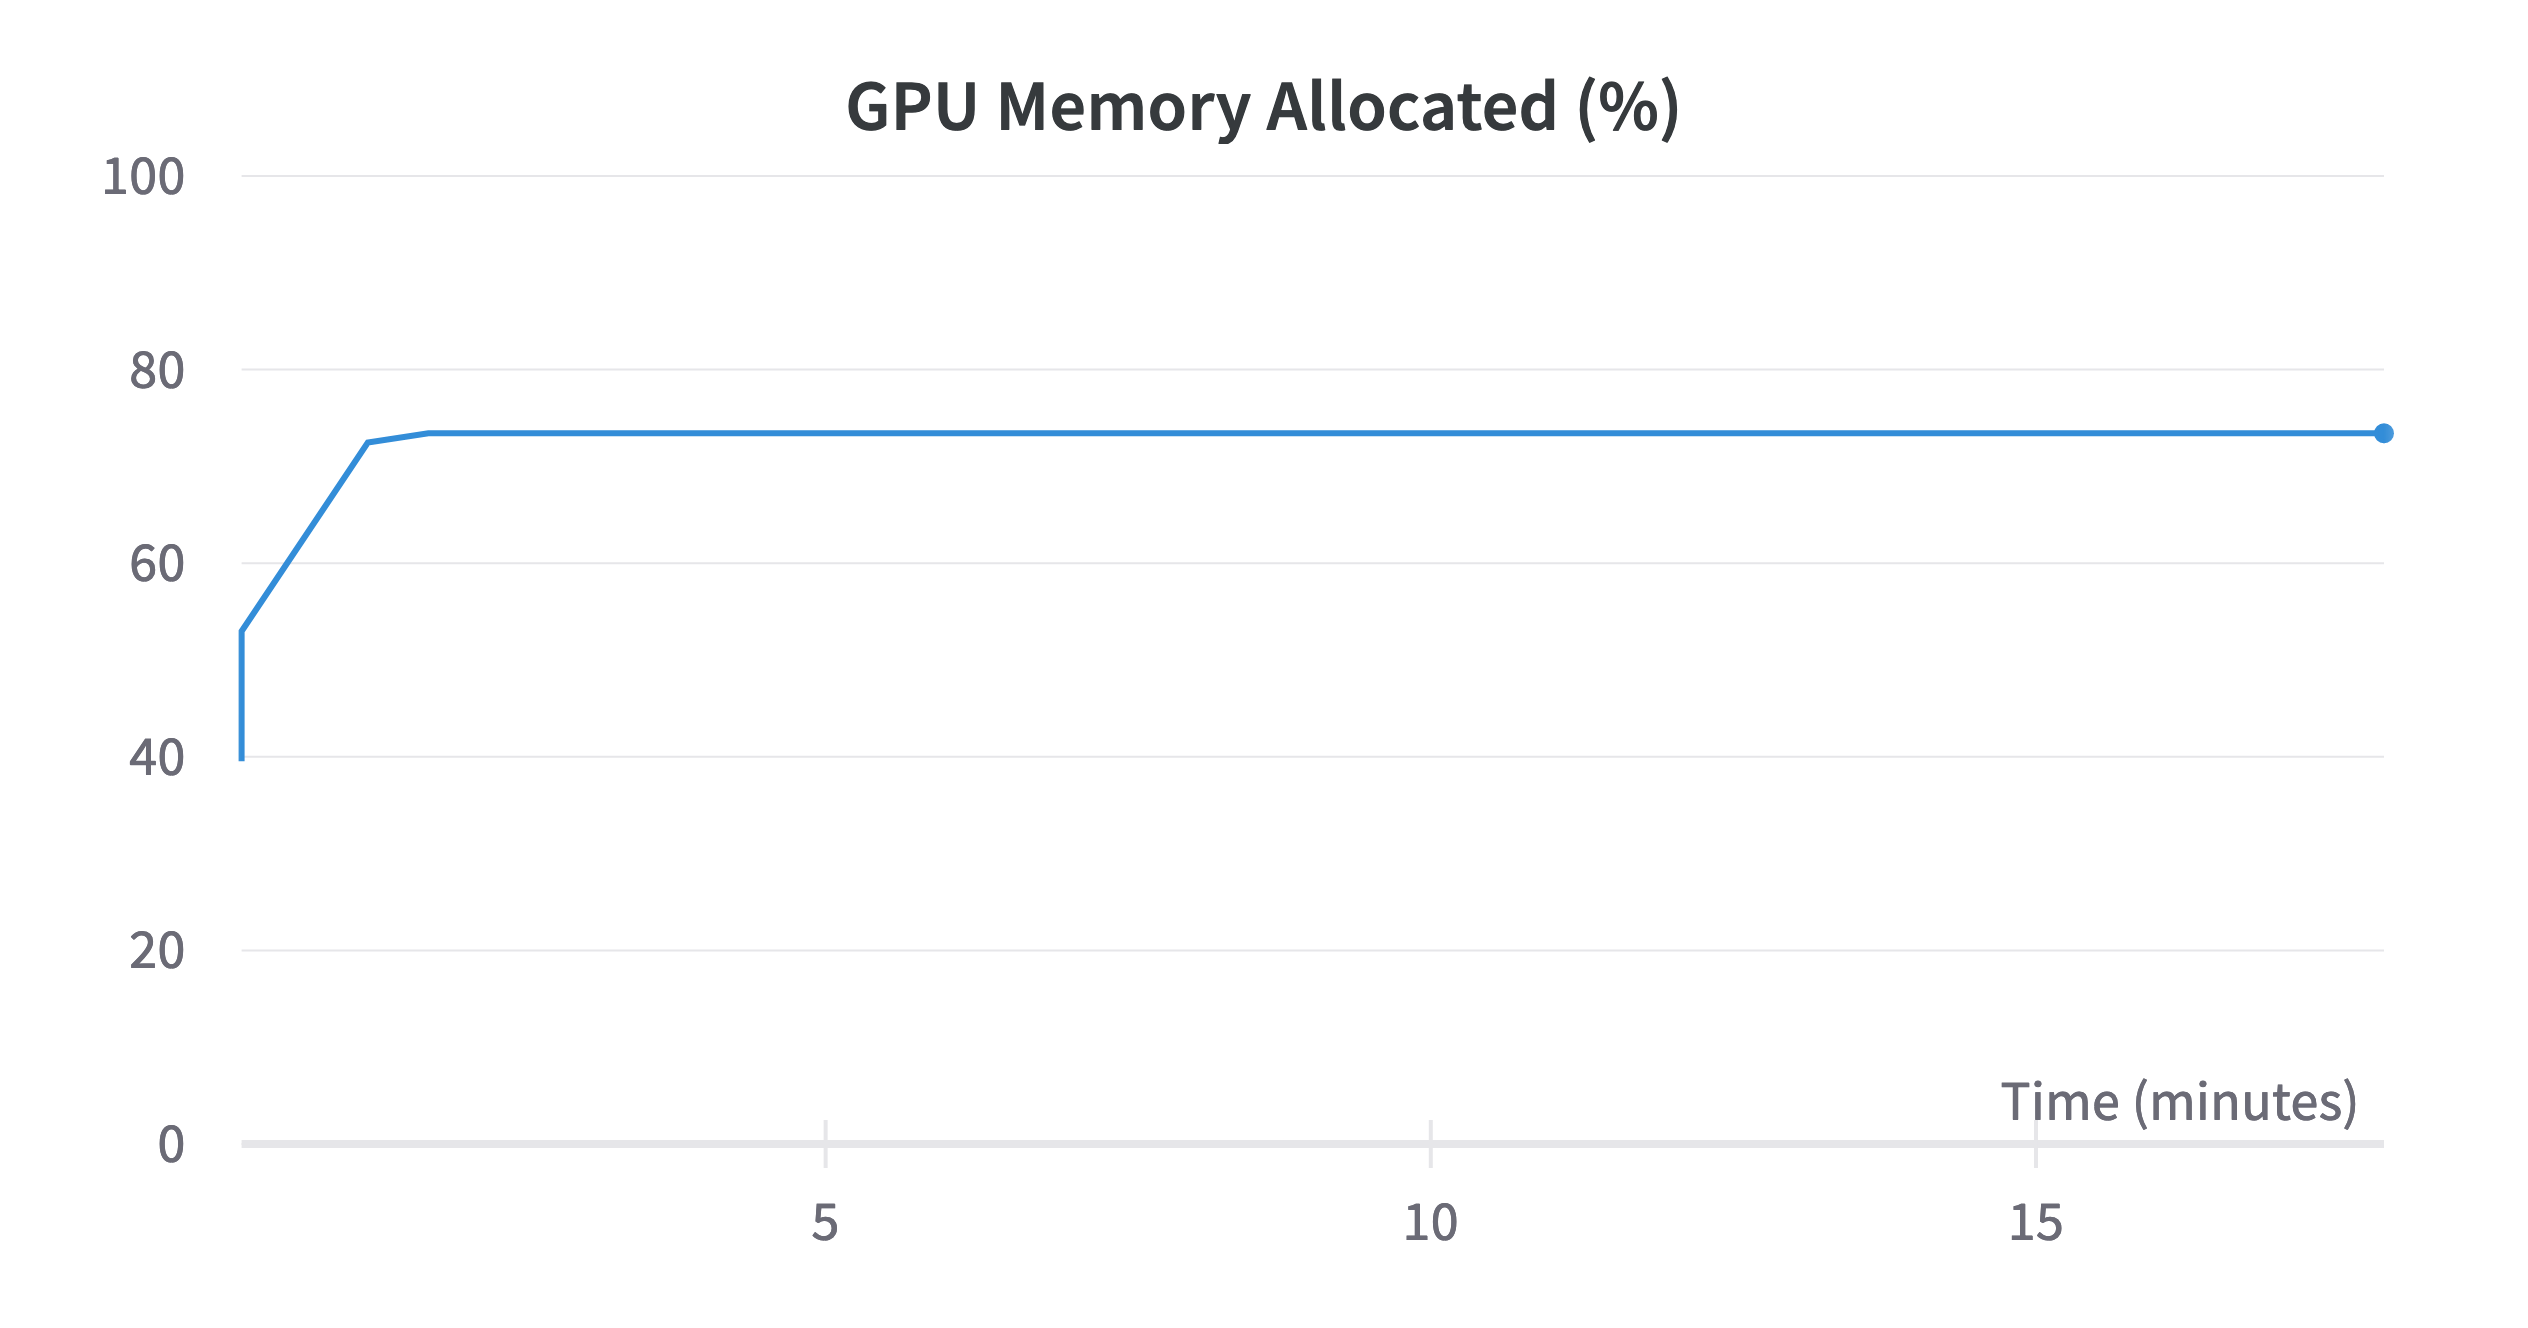
\includegraphics[width=\textwidth]{chapters/3_models/imgs/gab/train/gabrielgpumemalloc.png}
	\end{subfigure}\\
	\caption{System resources utilized during the Training phase.}
	\label{fig:gabsysusage}
\end{figure}


\begin{algorithm}[H]
	\caption{Transformer based model Training Algorithm}\label{alg:gabtraining}
	\begin{algorithmic}
		\Require train/validation datasets; Transformer based Neural Network Model

		\State Batch Size $\gets$ 8
		\State Learning Rate $\lambda \gets$ 0.00001
		\State Epochs $\gets$ 100
		\State Patience $\gets$ 20
		\State loss $\gets$ L1Loss()
		\State Optimizer $\gets$ AdamW Optimizer
		\State Scheduler $\gets$ CosineAnnealingScheduler
		\State Min Gap size $\gets$ 2 timestamps
		\State Max Gap size $\gets$ $\frac{\text{week length}}{3}$ timestamps
		\State
		\For{\textbf{each} epoch \textbf{in} epochs}
		\For{\textbf{each} (batch\_id, src\_data, tgt\_data, mask) \textbf{in} train.next\_batch()}

		\State train\_prediction $\gets$ model(src\_data) \Comment{Model inference}
		\State train\_prediction $\gets$ train\_prediction $\cdot$ mask
		\State train\_prediction $\gets \frac{\text{train\_prediction} \cdot \sum\text{train\_prediction}}{\sum tgt\_data}$ \Comment{Area normalization}
		\State train\_loss $\gets$ loss(train\_prediction[mask = 1], tgt\_data[mask = 1])
		\State Optimizer step
		\State Back Propagation
		\EndFor
		\State Scheduler step
		\State stop computing gradient
		\For{\textbf{each} (batch\_id, vs, vt, vm) \textbf{in} validation.next\_batch()}
		\State val\_prediction $\gets$ model(vs) \Comment{Model inference}
		\State val\_prediction $\gets$ val\_prediction $\cdot$ vm
		\State val\_prediction $\gets \frac{\text{val\_prediction} \cdot \sum\text{val\_prediction}}{\sum vt}$ \Comment{Area normalization}
		\State val\_loss $\gets$ loss(val\_prediction[vm = 1], vt[vm = 1])
		\EndFor

		\State check for Early Stopping
		\State check for Save Best Result
		\State start computing gradient
		\EndFor
	\end{algorithmic}
\end{algorithm}
\newpage
From the graph shown in Figure~\ref{fig:gabtrainchart}, we can observe that the training and validation loss curves, after an initial descent, remain relatively constant, and most importantly, they do not seem to diverge from each other. This indicates that the training phase has concluded successfully, with the validation loss value being lower by 0.01 compared to the RNN-based model.

From the graphs in Figure~\ref{fig:gabsysusage}, which show the machine's usage during the training phase, and from Table~\ref{tab:gabspecs}, it can be inferred that the model utilizes almost all of the available hardware resources, suggesting that it is computationally intensive and might be challenging to train on less powerful machines. However, it's essential to note that the inference time is extremely fast, not exceeding one second, and the model file size is very compact, with a dimension of approximately 2 MB.

%\newpage
\newpage
\section{Model Comparisons}
In this final section, we will compare the three models discussed in this thesis, analyzing their training phases, performance during testing phase, and identifying their strengths and weaknesses through the previous evaluation phase. We will determine which of these models is more suitable for solving the problem of time series imputation of photovoltaic data. It's essential to specify that to perform these comparisons, we reran the evaluation phase, fixing the gap size at 2 days and recalculating the various metrics used.

%In questa ultima sezione andremo a confrontare i tre modelli discussi in questa tesi, mettendo a confronto le loro fasi di training, performance ottenute durante la fase di testing, pregi e difetti individuati tramite la precedente fase di valutazione. Andremo quindi a vedere quale tra questi risulterà essere più adatto
%alla risoluzione del problema dell'imputazione di serie temporali di dati fotovoltaici. E' importante specificare che per effettuare questi confronti è
%stata rieseguita la fase di valutazione fissando la gap size a 2 giorni e ricalcolando le varie metriche impiegate.
%

\begin{table}[H]
	\centering
	\begin{tabular}{l|c|c|c|c}
		             &
		\makecell{\textbf{Model Size}                                   \\\textbf{(KB)}}
		             & \makecell{\textbf{Train Time}                    \\\textbf{(s)}}&
		\makecell{\textbf{GPU Usage}                                    \\\textbf{(\%)}} &
		\makecell{\textbf{CPU Usage}                                    \\\textbf{(\%)}}\\
		\hline
		\textbf{MLP} & 101.30                        & 24.00  & 20 & 10 \\
		\textbf{RNN} & 366.60                        & 49.00  & 20 & 27 \\
		\textbf{TRN} & 2400.0                        & 900.00 & 96 & 56
	\end{tabular}
	\caption{The table presents some data obtained during the training phase of each model.}
	%Nella tabella sono riportiati alcuni dati ottenuti durante la fase di addestramento di ogni modello.}
	\label{tab:cmptrainphase}
\end{table}

Analyzing the data shown in Table~\ref{tab:cmptrainphase}, we can see that the fastest and lightest model to train is the MLP-based one, followed by the RNN-based architecture, and finally, the Transformer. As seen in the previous sections, the first two models can certainly be trained on less powerful hardware compared to the available one, while it might be challenging for the last model. However, it's important to note that the inference time for each model is less than a second.

For all three models, the training phase was successfully completed without encountering significant issues. Comparing the graphs showing the training and validation loss curves, as shown in Figure~\ref{fig:ufcntraining}, \ref{fig:grruntraining}, and \ref{fig:gabtrainchart}, we can see that the best one is the Transformer-based model with a final validation loss value of 0.02, which is 0.01 lower than that of the RNN-based model.
%Analizzando i dati mostrati nella Tabella~\ref{tab:cmptrainphase} possiamo vedere che il modello più leggero e veloce ad addestrare risulta essere quello basato su MLP, segito poi dall'architettura che sfrutta le RNN ed infine il Transformer. Come anche visto nelle precedenti sezioni, i primi due modelli potrebbero essere sicuramente addestrati anche su architetture meno perfomanti di quella a nostra disposizione, mentre per l'ultimo probabilmente potrebbe essere molto difficile. Ricordiamo però che il tempo di inferenza per ognuno risulta essere inferiore al secondo di tempo.

%Per tutti e tre i modelli la fase di training è conclusa con successo senza riscontrare particolari problematiche. Confrontando i grafici che mostrano le curve della training e validation loss, riportati in Figura~\ref{fig:ufcntraining}, \ref{fig:grruntraining} e \ref{fig:gabtrainchart}, possiamo vedere come la migliore risulta essere quella del modello basato su Transformer con un valore finale della validatin loss di 0.02, inferiore di 0.01 rispetto a quella del modello basato su RNN.

\begin{table}[H]
	\centering
	\begin{tabular}{l|c|c|c|c|c}

		                   & \textbf{MLP}    & \textbf{RNN}    & \textbf{TRN}   & \multicolumn{2}{c}{\textbf{Incr. Gain (\%)}}         \\
		%\textbf{Model} & \textbf{MAE (kW)} & \textbf{MAPE (\%)} & \textbf{R$^2$} \\
		\hline
		                   &                 &                 &                & RNN                                          & TRN   \\
		\cline{5-6}
		\textbf{MAE (kW)}  & 14.11$\pm$3.81  & 6.86$\pm$1.87   & 3.76$\pm 0.39$ & 51.38                                        & 45.18 \\
		\textbf{MAPE (\%)} & 70.98$\pm$27.99 & 28.83$\pm$10.02 & 18.14$\pm$6.76 & 59.38                                        & 30.07 \\
		\textbf{R$^2$}     & 0.69$\pm$0.17   & 0.92$\pm$0.06   & 0.98$\pm$0.02  & 25.00                                        & 6.12

		%MAE (kW) & 14.11$\pm$3.81 & 70.98$\pm$27.99 & 0.69$\pm$0.17\\
		%MAPE (\%) &6.86$\pm$1.87 &28.83$\pm$10.02 &0.92$\pm$0.06\\
		%R$^2$ & 3.76$\pm 0.39$ &18.14$\pm$6.76 & 0.98$\pm$0.02
	\end{tabular}
	\caption{In the table, you can find the average values of MAE, MAPE, and the $R^2$ index for the three models, along with their respective standard deviations. Additionally, the Incremental Gain is provided, showing the percentage increase of the RNN model compared to MLP and the Transformer compared to RNN.}
	%Nella tabella sono riportati i valori medi del MAE, MAPE e indice $R^2$ dei tre modelli con la relativa deviazione standard. Viene inoltre mostrato l'Incremental Gain che riporta l'incremento in percentuale del modello RNN confronto al MLP e del Transformer confronto l'RNN.}
	\label{tab:comglobalmetrics3modelli}
\end{table}


\begin{figure}[H]
	\centering
	\begin{subfigure}{\textwidth}
		\centering
		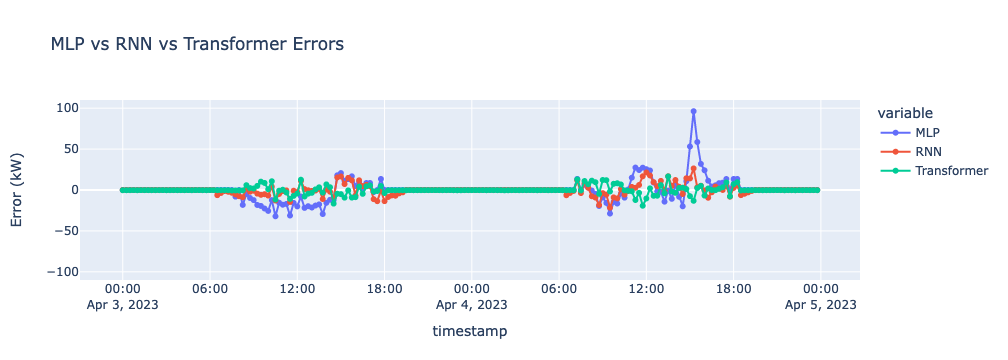
\includegraphics[width=\textwidth]{chapters/4_evaluation/imgs/cmp1.png}
		\caption{}
	\end{subfigure}
	%\begin{subfigure}{\textwidth}
	%    \centering    
	%    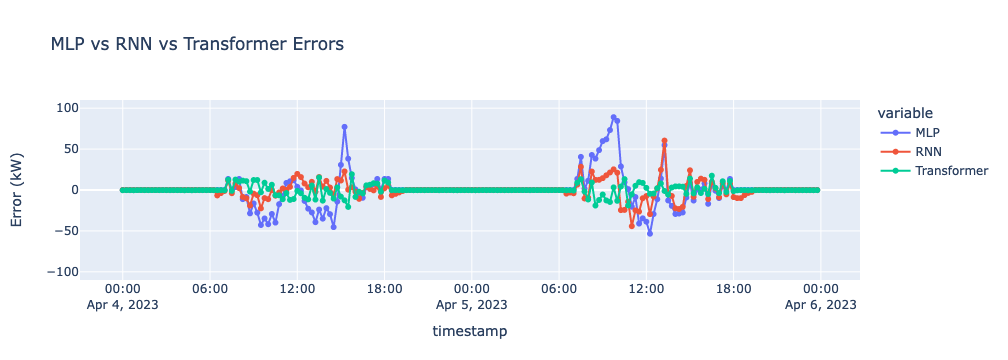
\includegraphics[width=.85\textwidth]{chapters/4_evaluation/imgs/cmp2.png}
	%    \caption{}
	%\end{subfigure}
	\begin{subfigure}{\textwidth}
		\centering
		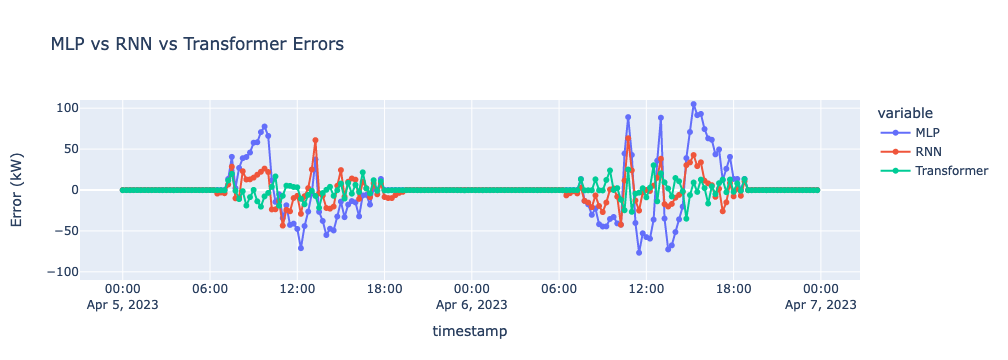
\includegraphics[width=\textwidth]{chapters/4_evaluation/imgs/cmp3.png}
		\caption{}
	\end{subfigure}
	\begin{subfigure}{\textwidth}
		\centering
		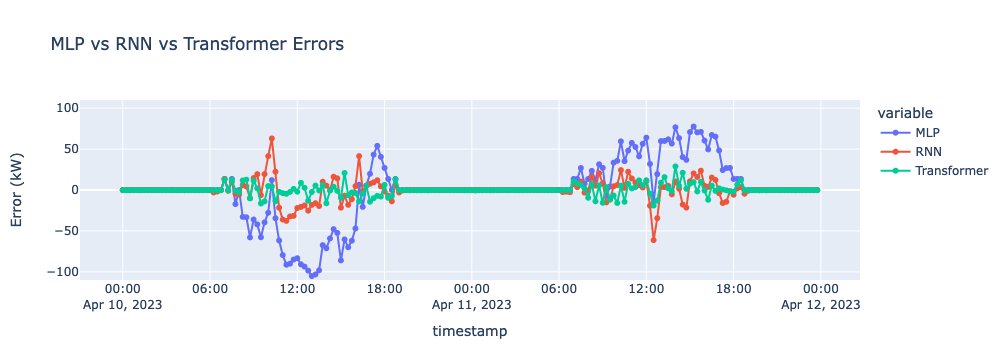
\includegraphics[width=\textwidth]{chapters/4_evaluation/imgs/cmp4.png}
		\caption{}
	\end{subfigure}
	\caption{The figure compares the errors made by the three models in predicting gaps with a two-day gap size. The blue curve represents the errors of the MLP-based model, the red curve represents the errors of the RNN-based model, and the green curve represents the errors of the Transformer-based model.}
	%Nella figura vengono paragonati gli errori commessi dai tre modelli nella predizione di buchi con gap size pari a due giorni. La curva in blu mostra gli errori commessi dal modello basato su MLP, la curva rossa fa riferimento agli errori del modello basato su RNN e quella verde del modello basato su Transformer.}
	%Nella figura sono mostrati alcuni risultati del modello ottenuti durante la fase di testing, utilizzando gap size di lunghezza variabile. Possiamo vedere gli output del modello (in rosso) confrontati con le relative ground truth (in blu).}
	\label{fig:cmperrs}
\end{figure}

Examining Table~\ref{tab:comglobalmetrics3modelli}, which shows the average values of MAE, MAPE, and the $R^2$ index for the various models, we can observe that the one based on the Transformer is significantly better. The RNN-based model is undoubtedly better than the MLP-based one, with the MAE value being 51\% lower and the MAPE showing an improvement of almost 60\%. The $R^2$ index has also improved by 25\%, indicating that the output of this model much better approximates the instantaneous energy values produced by the plant during 2-day gap periods.

However, the Transformer-based architecture excels in this task, with a 45\% improvement in MAE compared to the RNN-based model, a 30\% improvement in MAPE, and a 6\% improvement in the $R^2$ index. This model performs significantly better in predicting the plant's instantaneous energy compared to the RNN-based model, with the added capability of better detecting and understanding the presence of production peaks even over significantly variable time intervals.

%Prendendo in esame la Tabella~\ref{tab:comglobalmetrics3modelli}, dove sono riportate i valori medi di MAE, MAPE e indice $R^2$ per i vari modelli, possiamo osservare come il migliore risulta essere decisamente quello basato su Transformer.
%Il modello basato su RNN è indubbiamente migliore di quello basato su MLP, infatti il valore del MAE è inferiore del 51\%, similmente per il MAPE che abbiamo un miglioramento di quasi il 60\%. Anche l'indice $R^2$ è migliorato del 25 \% suggerendoci ce l'output di questo modello approssima nettamente meglio i valori dell'energia istantanea prodotta dall'impianto durante periodi di buchi di 2 giorni.
%
%L'architettura basata su Transformer eccelle però in questo compito avendo un MAE migliore del 45\% rispetto al modello basato su RNN, un miglioramento del 30\% sul MAPE e del 6\% sull'indice $R^2$. Questo modello riesce
%sicuramente meglio nel predirre l'energia istantanea dell'impianto rispetto all'RNN, avendo anche la capacità di individuare e comprendere molto meglio la presenza di eventuali picchi di produzione anche su intervalli di tempo notevolmente variabili.

\begin{table}[H]
	\centering
	\begin{tabular}{l|c|c|c}
		             & \textbf{AVG MAE (kW)} & \textbf{AVG Min Err (kW)} & \textbf{AVG Max Err (kW)} \\
		\hline
		\textbf{MLP} & 13.91                 & 0.35                      & 96.81                     \\
		\textbf{RNN} & 7.14                  & 0.20                      & 65.56                     \\
		\textbf{TRN} & 3.76                  & 0.12                      & 26.39
	\end{tabular}
	\caption{The table displays the average values of the metrics presented in Table~\ref{tab:cmperrtab}.}
	% Nella tabella sono riportate i valori medi delle metriche presenti nella Tabella~\ref{tab:cmperrtab}.}
	\label{tab:cmpavgdiffs}
\end{table}

These statements are supported by the graphs presented in Figure~\ref{fig:cmperrs} and the corresponding data in Tables~\ref{tab:cmperrtab} and \ref{tab:cmpavgdiffs}. The graphs illustrate the differences in point errors made by the various models. From these, we can see that the Transformer's errors (green line) are extremely compact and often close to the ideal value of 0, with an average value of 3.76 kW. The model based on RNN also has a similar curve (red line) but with values slightly farther from the ideal value and occasional error peaks, with an average value of 7.14 kW. The model based on MLP shows the worst error curve, often significantly deviating from the value of 0, featuring high error peaks, and having an average value of 13.91 kW.

We can also observe that the model based on the Transformer has a much lower average maximum point error, at 26.40 kW, compared to the RNN at 65.55 kW and the MLP at 98.81 kW. Similarly, for the average minimum point error, the Transformer-based architecture consistently performs the best, with an average value of 0.12 compared to 0.20 for RNN and 0.35 for MLP.
%Queste affermazioni vengono supportante anche dai grafici presenti in Figura~\ref{fig:cmperrs} e dai relativi dati in Tabella~\ref{tab:cmperrtab} e \ref{tab:cmpavgdiffs}.
%I primi mostrano le differenze tra gli errori puntuali commessi dai vari modelli. Da questi possiamo vedere come gli errori del Transformer (linea verde) risultano essere estremamente compatti e molto spesso vicini al valore ideale 0, con un valor medio di 3.76 kW. Anche il modello basato su RNN presenta
%una curva simile (linea rossa) ma con valore leggermente più distanti dal valore ideale con anche la presenza di qualche picco di errore e un valor medio di 7.14 kW. La curva degli errori peggiore è indubbiamente quella del modello basato su MLP che risulta molto spesso distante dal valore 0 con elevati picchi di errore e con un valore medio di 13.91 kW.
%
%Possiamo anche notare come il modello basato su Transformer ha come valor medio per il messimo errore puntuale commesso 26.40 kW decisamente molto inferiore rispetto a quello dell'RNN che è di 65.55 kW e quello dell'MLP di 98.81 kW. 
%Similmente per il minimo errore puntuale commesso dai modelli abbiamo che il migliore risulta essere sempre l'architettura basata su Transformer con un valore medio di 0.12 rispetto a quello di 0.20 e 0.35 per RNN e MLP.
%


\begin{table}[H]
	\centering
	\begin{subfigure}{\textwidth}
		\centering
		\begin{tabular}{l|l|l|l|l|l}
			\multicolumn{1}{c|}{\textbf{Gap}} & \multicolumn{3}{c|}{\textbf{MAE (kW)}}
			                                  & \multicolumn{2}{c}{\textbf{Incr. Gain (\%)}}                                                             \\
			\hline
			                                  & \textbf{MLP}                                 & \textbf{RNN} & \textbf{TRN} & \textbf{RNN} & \textbf{TRN} \\
			\cline{2-6}
			03-04 to 04-04                    & 6.90                                         & 3.65         & 2.73         & 47.10        & 25.21        \\
			04-04 to 05-04                    & 10.41                                        & 5.87         & 3.72         & 43.61        & 36.63        \\
			05-04 to 06-04                    & 17.99                                        & 7.83         & 4.25         & 56.48        & 45.72        \\
			10-04 to 11-04                    & 22.14                                        & 6.90         & 3.88         & 68.83        & 43.76
		\end{tabular}
		\caption*{(a)}
		%\vspace{1cm}
		%\caption{Nella tabella è riportato, per ogni modello, il valore del MAE (kW) nel relativo periodo in cui sono stati testati. Inoltre viene anche mostrato il valore dell' Incremental Gain in percetale del modello RNN rispetto a quello MLP e del Transformer rispetto all'RNN. Questi dati fanno riferimento ai grafici di Figure~\ref{fig:cmperrs}.}
		%\label{tab:compmae}
	\end{subfigure}
	%\vspace{1cm}
	\begin{subfigure}{\textwidth}
		\centering
		\begin{tabular}{l|l|l|l|l|l}
			\multicolumn{1}{c|}{\textbf{Gap}} & \multicolumn{3}{c|}{\textbf{Min. Err. (kW)}}
			                                  & \multicolumn{2}{c}{\textbf{Incr. Gain (\%)}}                                                             \\
			\hline
			                                  & \textbf{MLP}                                 & \textbf{RNN} & \textbf{TRN} & \textbf{RNN} & \textbf{TRN} \\
			\cline{2-6}
			03-04 to 04-04                    & 0.10                                         & 0.05         & 0.04         & 50.00        & 20.00        \\
			04-04 to 05-04                    & 0.20                                         & 0.14         & 0.05         & 30.00        & 64.28        \\
			05-04 to 06-04                    & 0.07                                         & 0.03         & 0.02         & 57.14        & 33.33        \\
			10-04 to 11-04                    & 0.19                                         & 0.13         & 0.10         & 31.57        & 23.07
		\end{tabular}
		\caption*{(b)}
	\end{subfigure}
	\begin{subfigure}{\textwidth}
		\centering
		\begin{tabular}{l|l|l|l|l|l}
			\multicolumn{1}{c|}{\textbf{Gap}} & \multicolumn{3}{c|}{\textbf{Max. Err. (kW)}}
			                                  & \multicolumn{2}{c}{\textbf{Incr. Gain (\%)}}                                                             \\
			\hline
			                                  & \textbf{MLP}                                 & \textbf{RNN} & \textbf{TRN} & \textbf{RNN} & \textbf{TRN} \\
			\cline{2-6}
			03-04 to 04-04                    & 96.28                                        & 26.38        & 19.22        & 72.60        & 27.14        \\
			04-04 to 04-05                    & 89.01                                        & 60.44        & 20.69        & 32.10        & 65.77        \\
			05-04 to 06-04                    & 105.01                                       & 63.29        & 35.10        & 39.73        & 44.54        \\
			10-04 to 11-04                    & 105.20                                       & 63.05        & 28.85        & 40.06        & 54.24
		\end{tabular}
		\caption*{(c)}
	\end{subfigure}
	\caption{In the table, the values of MAE (a), Minimum Error (b), and Maximum Error (c) are reported for each model in their respective testing periods. Additionally, the Incremental Gain in percentage is also shown for the RNN compared to the MLP and the Transformer compared to the RNN. These data correspond to the graphs in Figure~\ref{fig:cmperrs}.}
	%Nelle tabella è riportato, per ogni modello, il valore del MAE (a), Minimo Errore commesso (b) e Massimo Errore commesso (c) nel relativo periodo in cui sono stati testati. Inoltre viene anche mostrato il valore dell' Incremental Gain in percetale del modello RNN rispetto a quello MLP e del Transformer rispetto all'RNN. Questi dati fanno riferimento ai grafici di Figure~\ref{fig:cmperrs}.}
	\label{tab:cmperrtab}
\end{table}

Finally, after the analysis presented in this chapter of the various models, we can conclude that the best model for solving the imputation problem with data from time series of photovoltaic plants, despite the somewhat resource-intensive training phase, is undoubtedly the one based on the Transformer. This is due to its low MAE and MAPE values, and its near-perfect $R^2$ index. Moreover, the RNN-based model performs reasonably well in this task and could be a good alternative if one is willing to accept a slightly higher overall error in exchange for a significantly faster and lighter training phase compared to the Transformer.

%Infine, dopo l'analisi riportata in questo capitolo dei vari modelli, possiamo concludere che il migliore per 
%risolvere il problema dell'imputation su dati provenienti da serie temporali di impianti fotovoltaici, nonostante la fase di training sia
%abbastanza onerosa in termini di risorse hardware, sia sicuramente quello basato su Transformer, dato il basso valore del MAE, MAPE e del quasi perfetto valore per l'indice $R^2$. Inoltre, anche il modello basato su RNN riesce abbastanza bene in questo compito e potrebbe essere una buona alternativa, se si accetta un errore generale leggermente più alto, al Transformer per la fase di addestramento notevolmente più veloce e leggera.

%\begin{table}[H]
%    \centering
%    \begin{tabular}{l|l|l|l|l|l}
%         \multicolumn{1}{c|}{\textbf{Gap}} & \multicolumn{3}{c|}{\textbf{Min. Err. (kW)}}
%         & \multicolumn{2}{c}{\textbf{Gain (\%)}}\\
%         \hline
%         & \textbf{MLP} & \textbf{RNN} & \textbf{TRN}& \textbf{RNN} & \textbf{TRN} \\
%            \cline{2-6}
%         03-04 to 04-04 & 0.10&0.05&0.04&&\\
%         04-04 to 05-04 &0.20&0.14&0.05&&\\
%         05-04 to 06-04&0.07&0.03&0.02&&\\
%         10-04 to 11-04 &0.19&0.13&0.10&&
%    \end{tabular}
%    \caption{Nella tabella è riportato, per ogni modello, il valore del Minimo Errore commesso nel relativo periodo in cui sono stati testati. Inoltre viene anche mostrato il valore dell' Incremental Gain in percetale del modello RNN rispetto a quello MLP e del Transformer rispetto all'RNN. Questi dati fanno riferimento ai grafici di Figure~\ref{fig:cmperrs}.}
%    \label{tab:compminerr}
%\end{table}
%
%\begin{table}[H]
%    \centering
%    \begin{tabular}{l|l|l|l|l|l}
%         \multicolumn{1}{c|}{\textbf{Gap}} & \multicolumn{3}{c|}{\textbf{Max. Err. (kW)}}
%         & \multicolumn{2}{c}{\textbf{Gain (\%)}}\\
%         \hline
%         & \textbf{MLP} & \textbf{RNN} & \textbf{TRN}& \textbf{RNN} & \textbf{TRN} \\
%            \cline{2-6}
%         03-04 to 04-04 & 96.28&26.38&19.22&&\\
%         04-04 to 04-05&89.01&60.44&20.69&&\\
%         05-04 to 06-04&105.01&63.29&35.10&&\\
%         10-04 to 11-04 &105.20&63.05&28.85 & &
%    \end{tabular}
%    \caption{Nella tabella è riportato, per ogni modello, il valore del Massimo Errore commesso nel relativo periodo in cui sono stati testati. Inoltre viene anche mostrato il valore dell' Incremental Gain in percetale del modello RNN rispetto a quello MLP e del Transformer rispetto all'RNN. Questi dati fanno riferimento ai grafici di Figure~\ref{fig:cmperrs}.}
%    \label{tab:compmaxerr}
%\end{table}

%We will now compare the experimental results obtained by the
%MLP and RNN-based models.
%To do this, we will retest both networks on the testing dataset,
%forcing the generation of gaps that are consistently two days
%long to facilitate comparison (see Section~\ref{sec:mlpbaseline}
%and Section~\ref{sec:rnnbasemodel}).
%We will compare their performance by calculating, for each of them,
%the pointwise error between ground truth and prediction.
%Additionally, we will compare the various other metrics used
%and discuss some strengths and weaknesses of each model.
%
%%Confronteremo ora i risultati sperimentali ottenuti
%%dai modelli basati su MLP e RNN. Per farlo andremo a testare nuovamente
%%le due reti sul dataset di testing forzando la generazione di buchi
%%sempre a 2 giorni, in modo tale da poter confrontare i risultati (vedi 
%%Sezione~\ref{sec:mlpbaseline} e \ref{sec:rnnbasemodel}). Metteremo quindi
%%a confronto le performance di questi andando a calcolare, per ognuno,
%%l'errore puntuale tra ground truth e predizione. 
%%Infine, oltre a confrontare tra di loro le altre varie metriche impiegate,
%%andremo a discutere alcuni punti di forza e debolezze di ogni modello.
%
%\begin{table}[H]
%    \centering
%    \begin{tabular}{l|l|l|l}
%    \multicolumn{1}{c}{} &
%            \multicolumn{2}{c}{\textit{lower is better}} & \\
%        \multicolumn{1}{c|}{\textbf{Gap}} &
%        \multicolumn{2}{c|}{\textbf{MAE (kW)}} &
%        \multicolumn{1}{c}{\textbf{Gain (\%)}}  \\ %% ((MLP - RNN)*100)/MLP
%        \hline
%        & \small \textbf{MLP} & \small \textbf{RNN} & \\
%        \cline{2-3}
%        02-04 to 03-04 & 18.63 & 3.91 &  79.01\\
%        03-04 to 04-04 & 06.90 & 3.29 &  52.31\\
%        04-04 to 05-04 & 10.41 & 5.55 &  46.68\\
%        05-04 to 06-06 & 17.99 & 6.89 &  61.70\\
%        06-04 to 07-04 & 20.07 & 6.78 &  66.21\\
%        07-04 to 08-04 & 14.77 & 9.25 & 37.37\\
%        08-04 to 09-04 & 15.82 & 7.85 & 50.39\\
%        09-04 to 10-04 & 10.30 & 5.82 & 43.49
%    \end{tabular}
%    \caption{This table highlights the difference between the error of the MLP-based model and the RNN-based model. The column \texttt{Gain (\%)} represents the absolute percentage difference between MLP MAE and RNN MAE.}
%    %In questa tabella viene messo in evidenza la differenza tra l'errore del modello basato su MLP e quello su Reti Ricorrenti. La colonna \texttt{Diff (kW)} è la differenza in valore assoluto tra MLP MAE e RNN MAE, mentre \texttt{Diff (\%)} è la differenza in percentuale.}
%    \label{tab:mlpvsrnndiff}
%\end{table}
%
%\begin{table}[H]
%    \begin{minipage}[t]{.45\textwidth}
%        \centering
%\begin{tabular}[t]{l|l|l|l}
%\multicolumn{1}{c}{} &
%            \multicolumn{2}{c}{\textit{lower is better}} & \\
%         \multicolumn{1}{c|}{\textbf{Gap}} &
%         \multicolumn{2}{c|}{\makecell{\textbf{Max Err.}\\\textbf{(kW)}}} & 
%         \makecell{\textbf{Gain}\\\textbf{(\%)}} \\
%         \hline
%         & \small \textbf{MLP} & \small\textbf{RNN} &\\
%         \cline{2-3}
%        02-04 to 03-04 &  90.74 & 35.74 & 60.61\\ %55.0 \\
%        03-04 to 04-04 &  96.29 & 21.69 & 77.47\\ %74.60\\
%        04-04 to 05-04 &  89.01 & 54.95 & 29.27\\ %26.06\\
%        05-04 to 06-06 &  105.01 & 53.91 & 48.66\\ %51.10\\
%        06-04 to 07-04 &  122.56 & 51.35 & 58.10\\%71.21\\
%        07-04 to 08-04 &  105.94 & 75.91 & 28.34\\ % 30.03\\
%        08-04 to 09-04 &  86.14 & 75.47 & 06.55\\%05.65\\
%        09-04 to 10-04 &  78.76 & 59.97 & 23.85%18.79
%    \end{tabular}
%    \caption*{(a)}
%    %\caption{Nella tabella viene mostrata la differenza tra i valori dell'indice $R^2$ per i due modelli.}
%    \end{minipage}%
%    \hfill
%    \begin{minipage}[t]{.45\textwidth}
%        \centering
%    \begin{tabular}[t]{l|l|l|l}
%            \multicolumn{1}{c}{} &
%            \multicolumn{2}{c}{\textit{lower is better}} & \\
%         \multicolumn{1}{c|}{\textbf{Gap}} &
%         \multicolumn{2}{c|}{\makecell{\textbf{Min Err.}\\\textbf{(kW)}}} & 
%         \makecell{\textbf{Gain}\\\textbf{(\%)}} \\
%         \hline
%         & \small \textbf{MLP} & \small\textbf{RNN} &\\
%         \cline{2-3}
%        02-04 to 03-04 & 7.58 & 0.90 & 88.12\\ %6.68 \\
%        03-04 to 04-04 & 0.79 & 0.05 & 93.67\\ %0.74 \\
%        04-04 to 05-04 & 0.39 & 0.85 & 50.11\\ %-0.46\\
%        05-04 to 06-06 & 1.45 & 0.05 & 96.55\\ %1.40 \\
%        06-04 to 07-04 & 4.84 & 0.13 & 97.31\\ %4.71 \\
%        07-04 to 08-04 & 1.73 & 1.39 & 19.65\\ %0.34 \\
%        08-04 to 09-04 & 5.19 & 0.89 & 82.85\\% 4.30\\
%        09-04 to 10-04 & 3.19 & 0.71  & 77.74\\ %2.48
%
%    \end{tabular}
%    \caption*{(b)}
%    \end{minipage}
%    \begin{minipage}{\textwidth}
%    \vspace{.1cm}
%        \centering
%    \begin{tabular}[t]{l|l|l|l}
%    \multicolumn{1}{c}{} &
%            \multicolumn{2}{c}{\textit{bigger is better}} & \\
%         \multicolumn{1}{c|}{\textbf{Gap}} &
%         \multicolumn{2}{c|}{\textbf{$R^2$}} &
%         \multicolumn{1}{c}{\textbf{Gain (\%)}} \\
%         \hline
%         & \small \textbf{MLP} & \small\textbf{RNN} &\\
%         \cline{2-3}
%        02-04 to 03-04 & 0.64 & 0.98 & 34.69\\ %-0.34\\
%        03-04 to 04-04 & 0.52 & 0.91 & 42.85\\ %-0.39\\
%        04-04 to 05-04 & 0.52 & 0.89 & 41.57\\%-0.37\\
%        05-04 to 06-06 & 0.42 & 0.91 & 53.84\\ %-0.49\\
%        06-04 to 07-04 & 0.62 & 0.95 & 37.73\\ %-0.33\\
%        07-04 to 08-04 & 0.78 & 0.91 & 14.28\\ %-0.13\\
%        08-04 to 09-04 & 0.55 & 0.85 & 35.29\\ %-0.30\\
%        09-04 to 10-04 & 0.42 & 0.78 & 46.15 %-0.36
%    \end{tabular}
%    \caption*{(c)}
%    \end{minipage}
%
%    \caption{The tables compare the results of the two models, highlighting the maximum pointwise error (a), the minimum pointwise error (b), and the $R^2$ index (c). For each metric, the absolute percentage difference is also shown.}
%    %Le tabelle mettono a confronto i risultati dei due modelli paragonando il massimo errore puntuale (a) espresso in kW, il minimo errore puntuale (b) espresso in kW e l'indice $R^2$ (c). Per ognuna viene mostrata anche la differenza tra i due valore ($MPL - RNN$).}
%\end{table}
%
%From the previous tables, it's evident that the RNN-based model achieves significantly higher $R^2$ values compared to the MLP-based model. On average, the RNN-based model's values hover around 0.90, while the MLP-based model is around 0.60, with an average difference of 30\%. The second model approximates the trend of instant energy production during gaps much better.
%
%In tables (a) and (b), it can be observed that the architecture utilizing RNN has maximum and minimum error values significantly lower than the MLP-based model. Regarding Gap MAE, the second model is also superior to the first by approximately 60\%, with significantly lower average errors.
%
%%Dalle precedenti tabelle possiamo vedere com il modello basato su RNN ottiene
%%predizioni con un indice $R^2$ molto superiore a quello del modello basato su MLP. In media i valori del primo si aggirano intorno a 0.90 mentre per 
%%il secondo siamo sul 0.60 con una differenza media di 0.30 punti. Il secondo modello approssima nettamente meglio l'andamento dell'energia istantanea prodotta durante i buchi. 
%%Dalle tabelle (a) e (b) si vede come l'architettura che sfrutta RNN 
%%ha valori di errore massimi e minimi decisamente più contenuti rispetto a quella che
%%si basa su MLP.
%%Anche per il Gap MAE possiamo vedere come il secodo modello
%%sia migliore rispetto al primo di circa il 60\% commettendo in media errori
%%nettamente più bassi rispetto all'altro.
%
%\begin{figure}[H]
%    \centering
%    \begin{subfigure}{\textwidth}
%    \centering
%    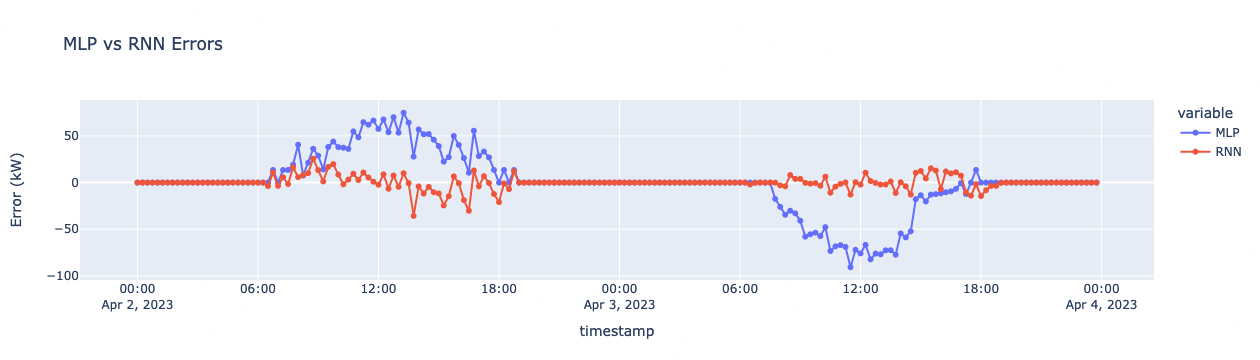
\includegraphics[width=\textwidth]{chapters/4_evaluation/imgs/mlpvsrnn/mlpvsrnn1.png}
%       \caption{} 
%    \end{subfigure}
%    \begin{subfigure}{\textwidth}
%    \centering
%    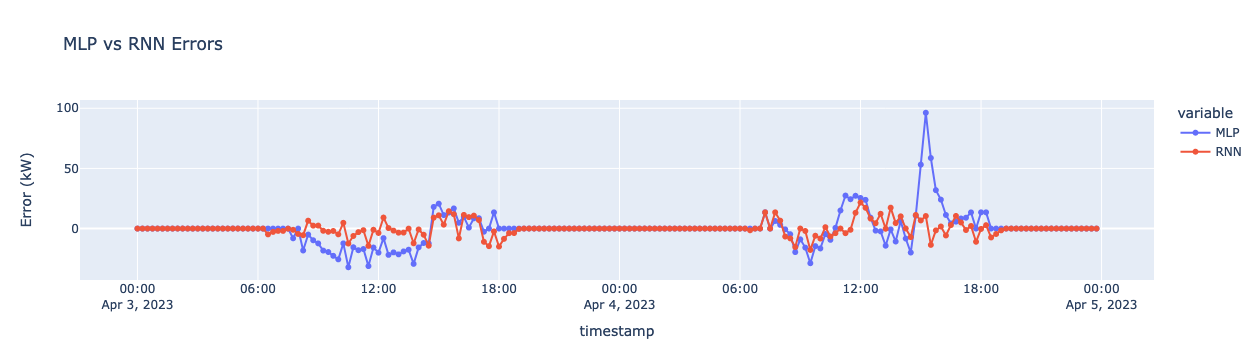
\includegraphics[width=\textwidth]{chapters/4_evaluation/imgs/mlpvsrnn/mlpvsrnn2.png}
%       \caption{} 
%    \end{subfigure}
%    \begin{subfigure}{\textwidth}
%    \centering
%    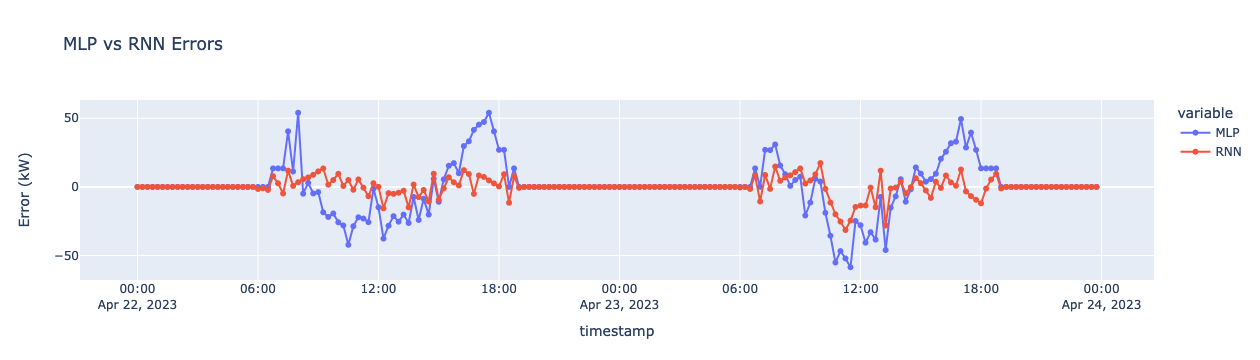
\includegraphics[width=\textwidth]{chapters/4_evaluation/imgs/mlpvsrnn/mlpvsrnn3.png}
%       \caption{} 
%    \end{subfigure}
%    \caption{The figure displays the difference curves between the target and prediction for the MLP-based models (in blue) and the RNN-based models (in red).}
%   % Nella figura sono mostrate le curve delle differenze tra target e predizione dei modelli basati su MLP (mostrate in blu) e su RNN (in rosso).}
%    \label{fig:mlpvsrnngrafici}
%\end{figure}
%From the graphs shown in Figure~\ref{fig:mlpvsrnngrafici},
%it's immediately noticeable that the architecture utilizing
%recurrent neural networks commits significantly lower errors
%than the MLP-based model.
%The red curves are generally more compact and closer to 0
%(no error committed), while the blue curves are on average
%much farther from the ideal value, indicating a significantly
%higher pointwise error, on average by 60\%, with the presence
%of substantial peaks (b).
%It's important to highlight that both models do not commit errors at night.
%
%Comparing the respective outputs of the two models,
%it's evident that the predicted curves by the MLP-based model
%are extremely similar to each other and fail to identify
%possible production peaks.
%On the other hand, the output of the second model
%performs significantly better in the task, generating curves
%that closely follow the ground truth, understanding the
%presence of potential energy peaks, and demonstrating the
%ability to generate curves with different shapes and widely
%varying values.
%
%It's also noticeable that the first model struggles with
%identifying day and night periods, often ending production a
%few hours before sunset.
%In contrast, the second model excels in understanding
%this alternation and does not exhibit issues of this nature.
%
%It's also important to note that both models are relatively
%lightweight in terms of resources for training and inference
%on the architecture at our disposal.
%This suggests the possibility of training and using
%them on less powerful machines.
%
%The second model can also close gaps of considerably larger
%sizes than those used during the training phase.
%In contrast, the first model can only handle 2-day gaps,
%and to increase this limit, the model would need to repeat
%the training phase.
%
%%Dai grafici mostrati in Figura~\ref{fig:mlpvsrnngrafici} possiamo 
%%notare immediatamente che l'architettura che sfrutta le reti ricorrenti
%%commette errori significativamente più bassi di quella basata su MLP.
%%Notiamo come le curve in rosso sono generalmente più compatte ed abbastanza
%%vicine allo 0 (nessun errore commesso). Mentre quelle in blu risultano mediamente
%%molto più distanti dal valore ideale evidenziando quindi un errore puntuale nettamente più alto, in media del 60\%, con la presenza di picchi di notevole valore (b). \'{E} importante evidenziare che di notte tutti e
%%due i modelli non commettono errori.
%
%%Confrontando i relativi output dei due modelli possiamo notare come
%%le curve predette dal modello basato su MLP siano estremamente simili
%%tra di loro e non riescono ad individuare possibili picchi di produzione.
%%Mentre l'output del secondo riesce nettamente meglio nel compito generando
%%curve che seguno bene l'andamento della ground trouth, riuscendo a comprendere
%%anche presenza di possibili picchi di energia prodotta oltre all'abilità
%%di generare curve di differente forma e valori anche moltro diversi
%%tra di loro.
%
%%Notiamo anche che il primo modello ha qualche difficoltà nel capire 
%%i periodi di giorno e notte con il risultato che molto spesso termina la 
%%produzione qualche ora prima del tramonto, mentre il secondo riesce molto
%%bene a comprendere questa alternanza e non presenta probemi di questo tipo.
%
%%\'{E} importante anche notare che tutti e due i modelli risultano relativamente
%%leggeri sia in termini di risorse per l'allenamento e per l'inferenza sull'architettura a nostra disposizione. Suggerendo quindi la possibilità
%%di essere addestrati ed usati anche su macchine meno performanti.
%
%%Il secondo modello riesce anche a chiudere buchi di dimensioni notevolmente
%%maggiori rispetto a quelli utilizzati durante la fase di training, mentre il primo riesce a gestire solo buchi di 2 giorni e per poter aumentare questo limite, il modello necessita di ripetere nuovamente la fase di trianing.
%
%\begin{figure}[H]
%    \centering
%    \begin{subfigure}{\textwidth}
%        \centering    
%        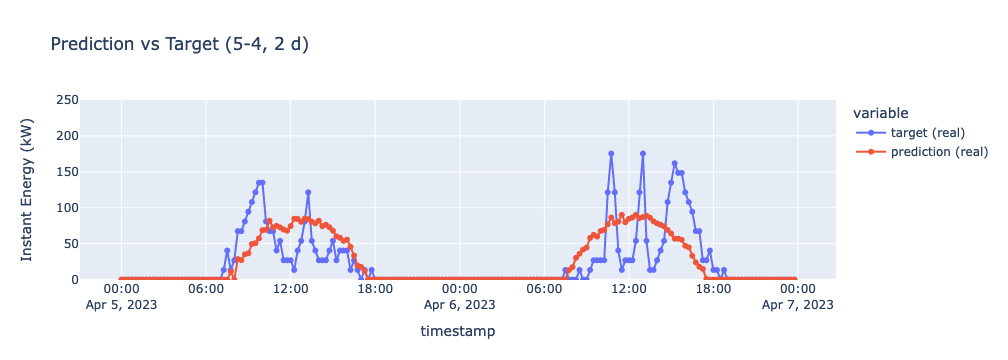
\includegraphics[width=.75\textwidth]{chapters/3_models/imgs/ufnc/eval/ufcpred5-4.png}
%        \caption{}
%    \end{subfigure}
%    \begin{subfigure}{\textwidth}
%        \centering    
%        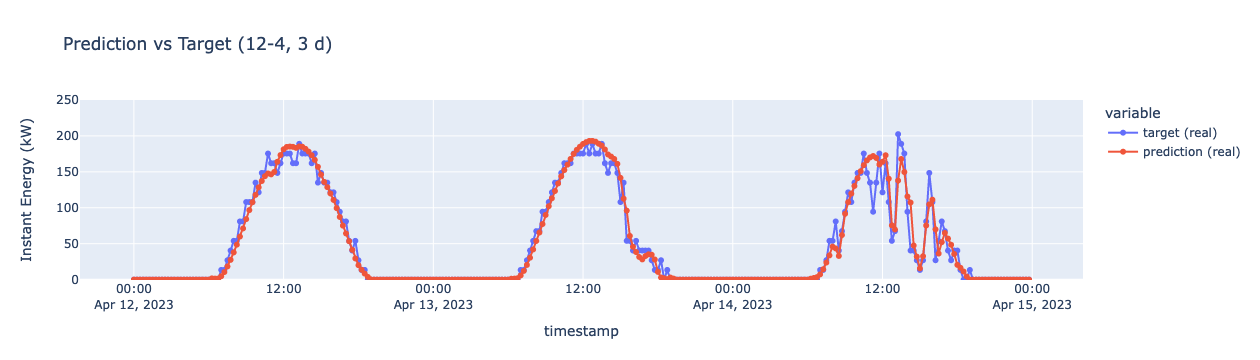
\includegraphics[width=.75\textwidth]{chapters/3_models/imgs/grrun/eval/grruneval124.png}
%        \caption{}
%    \end{subfigure}
%    \caption{Visual comparison between an output of the MLP-based model (a) and an output of the RNN-based model (b).}
%    %Confronto visuale tra un output del modello basato su MLP (a) e output del modello basato su RNN (b).}
%\end{figure}
%    
%\section{Final Conclusions}
In conclusion, the models described and evaluated in this work have shown varying degrees of success in predicting the instant energy production curve of the plant during gaps. The Recurrent Neural Network-based model, despite being lightweight and efficient, demonstrated limited ability to generalize and predict production variations effectively. It struggled to capture the possibility of production spikes and had difficulty managing the day/night cycle.

While the Unified Fully Connected Network model showed promise, especially in capturing some of the energy production variations, it, too, had limitations when faced with more complex and variable patterns. Both models displayed difficulties in handling gaps of differing sizes.

Overall, the models provide valuable insights into energy production trends, and their predictability can be useful in certain contexts. However, further model refinement and optimization, along with the introduction of techniques that can handle variable gap sizes and more complex patterns, may be necessary to achieve more accurate and reliable predictions. Additionally, expanding the dataset and applying advanced techniques for time series prediction could contribute to more successful models in the future.